\documentclass[a4paper,12pt]{report}
% \documentclass[a4paper,fleqn,twoside,12pt]{report}


\usepackage[]{geometry}
% \usepackage[latin1]{inputenc}
\usepackage[utf8]{inputenc}
\usepackage[UKenglish]{babel}
\usepackage[UKenglish]{isodate}
\usepackage{amsmath}
\usepackage{amsfonts}
\usepackage{amssymb}
\usepackage{amsthm}
\usepackage{graphicx}
\usepackage{chngpage}
\usepackage{calc}
\PassOptionsToPackage{hyphens}{url}
\usepackage{hyperref}
\usepackage[nameinlink]{cleveref}
\usepackage{fancyhdr}
\usepackage{titletoc}
\usepackage[explicit]{titlesec}
% \usepackage{natbib}
\usepackage[dvipsnames, table]{xcolor}
\usepackage[sc]{mathpazo}
\linespread{1.05}
\usepackage[T1]{fontenc}
\usepackage{minted}

% TODO: Check packages for needed/uneeded
% TODO: Play with formatting (e.g. french spacing) and margins
% \usepackage[toc,page]{appendix}
\usepackage{tikz}
\usepackage{pgfplots}
% https://github.com/nschloe/tikzplotlib
\DeclareUnicodeCharacter{2212}{−}
\usepgfplotslibrary{groupplots,dateplot}
\usetikzlibrary{patterns,shapes.arrows}
\pgfplotsset{compat=newest}

% https://tex.stackexchange.com/a/53540
\usepackage{caption}
\newenvironment{code}{\captionsetup{type=listing}}{}
\setminted{  
% frame=lines,
% framesep=2mm,
% baselinestretch=1.2,
% bgcolor=lightergray,
% fontsize=\footnotesize,
linenos,
breaklines,
autogobble
}  

\hypersetup{
	colorlinks=true,
	linkcolor=black,
	urlcolor=black,
	citecolor=black
}

\setlength{\parindent}{0mm}
\setlength{\parskip}{\medskipamount}
\renewcommand\baselinestretch{1.2}

\cleanlookdateon

\makeatletter
\newcommand{\@assignment}[0]{Assignment}
\newcommand{\assignment}[1]{\renewcommand{\@assignment}{#1}}
\newcommand{\@supervisor}[0]{}
\newcommand{\supervisor}[1]{\renewcommand{\@supervisor}{#1}}
\newcommand{\@yearofstudy}[0]{}
\newcommand{\yearofstudy}[1]{\renewcommand{\@yearofstudy}{#1}}
\makeatletter

\pagestyle{plain}
\renewcommand{\headrulewidth}{0.0pt}

\makeatletter
\fancypagestyle{plain}{
	\fancyhf{}
	% \fancyhead[LE]{\thepage}
	% \fancyhead[RE]{\textit{\@author}}
	% \fancyhead[RO]{\thepage}
	% \fancyhead[LO]{\textit{\@title}
	\fancyhead[R]{\thepage}
	\fancyhead[L]{\textit{Assessing the suitability of Rust for performant and productive\\ implementations of HPC codebases}}
}
\makeatother


\author{Edmund Goodman}
\yearofstudy{3\textsuperscript{rd}} % year, excluding industrial placement
\title{Assessing the suitability of Rust for performant and productive implementations of HPC codebases}
\supervisor{Dr Richard Kirk}

\showthe\font
%%%%%%%%%%%%%%%%%%%%

% https://warwick.ac.uk/fac/sci/dcs/teaching/material/cs310/components/final/format/
% https://warwick.ac.uk/fac/sci/dcs/teaching/material/cs310/components/final/marking/technical
% https://warwick.ac.uk/fac/sci/dcs/teaching/material/cs310/components/final/marking/communication

\begin{document}

%TC:ignore
% \makeatletter
% \begin{titlepage}
%     % \textbf{\Huge \@title} \\[1.5cm]
%     % \Large \textbf{\@author} \\
%     % Department of Computer Science \\
%     % University of Warwick \\
%     % \newline
%     % \ifdefempty{\@supervisor}{}{
%     %     Supervised by \@supervisor \\
%     % }
%     % \ifdefempty{\@yearofstudy}{}{
%     %     Year of Study: \@yearofstudy \\
%     % }

%     % \vfill
%     % \today

%     % \begin{adjustwidth}{-\oddsidemargin-1in}{-\rightmargin}
%     %     \centering
%     %     
\includegraphics[width=\paperwidth]{images/_title_page/line.png}
%     % \end{adjustwidth}
%     % \vspace*{-3.5cm}
% \end{titlepage}
% \makeatother

\newgeometry{margin=0pt}

\includegraphics{images/_title_page/title_page.pdf}
\restoregeometry
% \clearpage


\pagestyle{plain}

\begin{abstract}
    Rust is a type-safe programming language originally developed by Mozilla in 2010. Since its first release, it has gained a large community of dedicated followers. Designed to be memory safe and have foundations in functional programming, it claims to be highly performant, safe, and provide a robust development toolchain.

    The aim for this project is to take a proxy application, for example from the Mantevo Suite, and translate it from C/C++ to Rust. Both versions should be multi-threaded and should be validated against each other for all inputs. Once this has been achieved, a performance study of both versions of the application would be required, contrasting the translated Rust against the original C/C++.

    An extension to this is to implement a Rust+MPI version of the application, and test this against an equivalent C/C++ version across a large amount of compute nodes.
\end{abstract}

% TODO: Change abstract to reflect work done not planned work (and focus more on workflow etc.)
% TODO: Add citations
% TODO: Add keywords

% TODO: Add acknowledgements (separate page)
% TODO: Add abbreviations/glossary (separate page)


% TODO: Make the way figures/tables are captioned consistent, e.g. not starting with ``a figure that shows?''
\tableofcontents
\listoffigures
\listoftables
\listoflistings
%TC:endignore

% TODO: Consider switching to include for performance?
% https://tex.stackexchange.com/questions/246/when-should-i-use-input-vs-include
% TODO: Move chapters into separate folders with their own image folders?
% TODO: Decide on sentence vs title case and be consistent throughout
\chapter{Introduction}
\label{ch:introduction} % 500 words

% Write around four paragraphs establishing the context and motivating your project.

% % TODO: Does this overlap with literature review?
% \section{Related work}
% \label{sec:related-work}

% Discuss related work.


\section{Objectives}
\label{sec:objectives}

% One sentence summary of your project. Followed by a short list of concrete objectives:

% \begin{itemize}
%     \item Objective 1
%     \item Objective 2
%     \item Objective 3
% \end{itemize}

\chapter{Background}
\label{ch:background}

% ``Everybody who learns concurrency thinks they understand it, ends up finding mysterious races they thought weren’t possible, and discovers that they didn’t actually understand it yet after all.'' -- Herb Sutter, chair of the ISO C++ standards committee, Microsoft.

The background for this project will provide a summary of relevant aspects of the Rust programming language and the field of \acrshort{HPC}, along with a literature review of existing performance analyses of Rust in \acrshort{HPC} applications.


\section{The Rust Language}
\label{sec:rust}

This section provides a description of salient features of the Rust language, which are required to understand the intricacies of the translation, equivalence checking, and performance analysis processes described in this project. Aspects of the content of this introduction are derived from Klabnik and Nichols' book ``The Rust Programming Language'' \cite{RustProgrammingLanguage}. This is the seminal text for beginners learning Rust, affectionately nicknamed ``the book'' within the Rust community \cite{LearnRust}.

\subsection{Basic syntax}
\label{ssec:rust-syntax}

In any programming language, the first program written tends to be printing ``Hello World'', a tradition introduced by Kernighan and Ritchie in the first chapter of ``The C Programming Language'' \cite{kernighan2002c}. In Rust, the ``Hello world'' program is shown in Listing \ref{listing:rust-hello-world}.

\begin{code}
    %TC:ignore
    \begin{minted}{rust}
        fn main() {
            println!("Hello, world!");
        }
    \end{minted}
    %TC:endignore
    \caption{Rust program to print ``Hello, world!'', derived from Listing 1-1 of ``The Rust Programming Language'' \cite{RustProgrammingLanguage}.}
    \label{listing:rust-hello-world}
\end{code}

The influence of the C-family of languages on Rust's syntax is clear, for example the use of braces and semicolons, along with the presence of a \mintinline{rust}{main} function.

% After having printed ``Hello World'', the next thing a programmer is likely to do in an imperative language is define a variable. However, this is where the influence of functional languages like Haskell and the ML-family begins to show -- variables in Rust are immutable by default. As chapter 3-1 of the Rust book states, this is ``one of the many nudges Rust gives you to write your code in a way that takes advantage of the safety and easy concurrency that Rust offers'' \cite{RustProgrammingLanguage}, since immutable variables are easier for the compiler to reason about to provide guarantees of memory safety.

% Variables in Rust are defined using the \mintinline{rust}{let} keyword, and can be explicitly marked as mutable when required using the \mintinline{rust}{mut} keyword. In addition to this, namespace shadowing can be used to redefine variables with new values, by re-using the \mintinline{rust}{let} keyword. Some of the semantics of Rust variables are shown in Listing \ref{}.

% % Type system
% Another aspect of Rust's pedigree from functional languages is its rich type system.

% % Iterators
% One of the many ergonomic features Rust provides is ``zero-cost abstractions''. This refers to high-level structures to perform common tasks, such as the \mintinline{rust}{fold} operation on vectors, which compiles down to the same, performant, assembly as a more verbose iterative expression of the same functionality. Zero-cost abstractions allow programmers to write terse code, whilst not sacrificing performance.

% One example of a zero-cost abstraction is Rust's iterators.


\subsection{Ownership model}
\label{ssec:rust-ownership}

As mentioned in the introduction, a core feature of Rust is its guarantees against undefined behaviour. These guarantees are provided in large part by its ownership model, enforced by an aspect of the compiler called the borrow checker \cite{ReferencesBorrowing}. Most languages employ one of two strategies for managing memory: garbage collection or manual memory management \cite{hertzQuantifyingPerformanceGarbage2005}. In garbage collected languages such as Java and Python, there is a runtime environment which executes alongside the program, allocating memory when required, and deallocating it when it is no longer in use. However, this additional overhead of the garbage collector running in parallel typically incurs a performance cost  \cite{hertzQuantifyingPerformanceGarbage2005}. In manual memory management, the allocation and deallocation of memory is explicitly controlled by the programmer. This avoids the runtime cost of the garbage collector, but can lead to errors and undefined behaviour if the programmer makes a mistake, such as double-free and use-after-free errors respectively.

Rust takes a third approach to memory management, enforcing a set of ownership rules checked by the compiler. By following these rules, the compiler can always infer when memory is no longer in use through scope or explicit lifetimes, and deallocate it as required. Furthermore, it provides strong guarantees against undefined behaviour as a result of invalid memory accesses and data races, since these are prohibited by the ownership rules. In ``The Rust Programming Language'' \cite{RustProgrammingLanguage}, Klabnik and Nichols summarise Rust's ownership model through three rules:

\begin{quote}
    \begin{enumerate}
        \item Each value in Rust has an owner.
        \item There can only be one owner at a time.
        \item When the owner goes out of scope, the value will be dropped.
    \end{enumerate}
\end{quote}

From the third rule of Rust's ownership model, we can see that memory management is based on lexical scopes, and the inferences which can be made about data lifetimes from them. Variables are valid for the scope in which they are defined, and as soon as the scope ends, Rust automatically ``drops'' the variable \cite{sautterOBSERVINGPARALLELEXECUTION}. This automatically performs an operation similar to the \mintinline{c}{free} function in C, hence avoiding all ``double-free'' memory management bugs. An example of scopes in Rust is shown in Listing \ref{listing:rust-scope}.

\begin{code}
    %TC:ignore
    \begin{minted}{rust}
        {
            // s is not valid here, it’s not yet declared
            let s = "hello";
            // s is valid from this point forward

            // do stuff with s
        }
        // this scope is now over, and s is no longer valid
    \end{minted}
    %TC:endignore
    \caption{Rust program to demonstrate the scope of variables, derived from Listing 4-1 of Klabnik and Nichols' ``The Rust Programming Language'' \cite{RustProgrammingLanguage}.}
    \label{listing:rust-scope}
\end{code}

The first two rules of Rust's ownership model enforce exclusive ownership of memory by a single variable. Whilst this guarantees memory safety, as only one variable has access to data at a time, it is incredibly restrictive \cite{sautterOBSERVINGPARALLELEXECUTION}. To mitigate this, Rust provides ``references'', which improve expressiveness whilst maintaining safety guarantees. In ``The Rust Programming Language'' \cite{RustProgrammingLanguage}, Klabnik and Nichols summarise the Rule's of borrowed references as:

\begin{quote}
    \begin{enumerate}
        \item At any given time, you can have either one mutable reference or any number of immutable references.
        \item References must always be valid.
    \end{enumerate}
\end{quote}

References allow the owner of a piece of data to explicitly hand over access to it via references, without giving up ownership. An arbitrary number of immutable references, denoted by \mintinline{rust}{&} and granting read-only access to the data, are allowed. However, only a single mutable reference, denoted by \mintinline{rust}{&mut} and granting both read and write access, is permitted. A corollary of this rule is the prohibition of data races in safe Rust, as only one variable can write to a value in memory at a time.

% \begin{code}
%     %TC:ignore
%     \begin{minted}{rust}
%     \end{minted}
%     %TC:endignore
%     \caption{Rust program to demonstrate the borrowing of variables through references.}
%     \label{listing:rust-scope}
% \end{code}

In some cases, the rules for borrowed references to guarantee memory safety are too restrictive to implement the desired functionality, which in other languages could be implemented using raw pointers. In this case, Rust provides smart pointers, which originated in C++, as structures which Klabnik and Nichols' define as ``act[ing] like a pointer but also hav[ing] additional metadata and capabilities'' \cite{RustProgrammingLanguage}. These are a general design pattern in Rust, with many different concrete implementations, each providing different properties.

Rust's enforcement of rules including the ownership model at statically at compile time provide strong guarantees of memory safety without impacting program performance. However, sometimes programmers need to be able to express functionality which violates these rules, such as dereferencing a raw pointer. This can be done through \mintinline{rust}{unsafe} Rust. As Klabnik and Nichols state, ``unsafe Rust exists because, by nature, static analysis is conservative'' \cite{RustProgrammingLanguage}. The details of unsafe Rust are beyond the scope of this introduction, but are covered by ``The Rustonomicon''  \cite{IntroductionRustonomicon}.

\subsection{Fearless concurrency}
\label{ssec:rust-fearless-concurrency}

One of the key design goals of the Rust language is ``handling concurrent programming safely and efficiently'' \cite{RustProgrammingLanguage}. Oracle defines concurrency as ``when at least two [tasks] are making progress'' \cite{DefiningMultithreadingTerms}. This includes both interleaved execution and true parallelism across multiple execution units.

At the start of Rust's development, memory safety and safe concurrency were considered to be two distinct problems. However, it was discovered that many of the strategies to guarantee memory safety, such as the ownership model and rich type system, also addressed common concurrency issues \cite{FearlessConcurrencyRust}. As a result of this, as with memory safety, many common concurrency bugs which would occur at runtime in languages like C++ are detected at compile time in Rust -- allowing for ``Fearless concurrency''.

Rust provides functions in its standard library to spawn threads and communicate between them, through both message passing and shared memory. In addition to this, empowered by ``Fearless concurrency'', there are a number of third-party libraries which provide utilities and further abstractions for writing concurrent code.

One such library is \texttt{rayon}, which describes itself as ``extremely lightweight and makes it easy to convert a sequential computation into a parallel one'' \cite{RayonRust}. \texttt{rayon} provides a drop-in mechanism to leverage parallelism for a common design pattern in Rust, iterators. Iterators allow you to lazily perform tasks over a sequence of items, and are commonly constructed using the \texttt{iter} function on vectors. \texttt{rayon} provides a mechanism to convert sequential iterators into parallel ones, with the \texttt{par\_iter} function. This is much like OpenMP providing compiler directives to parallelise loops, but with the added benefit of guarantees against common bugs such as data races.

\subsection{Toolchain and infrastructure}
\label{ssec:rust-toolchain}

A final key feature of Rust is its strong development toolchain. Firstly, Rust very simple to install and update using the \texttt{rustup} tool. Installation does not require elevated privileges, and requires only a single command -- lowering the barrier to entry for using the language. Once Rust is installed, its compiler \texttt{rustc} is well known for its verbose and clear error messages, which typically contain suggestions on how to fix errors when they occur, as shown in Figure \ref{fig:rust_error_messages}.

\begin{figure}[H]
    \centering
    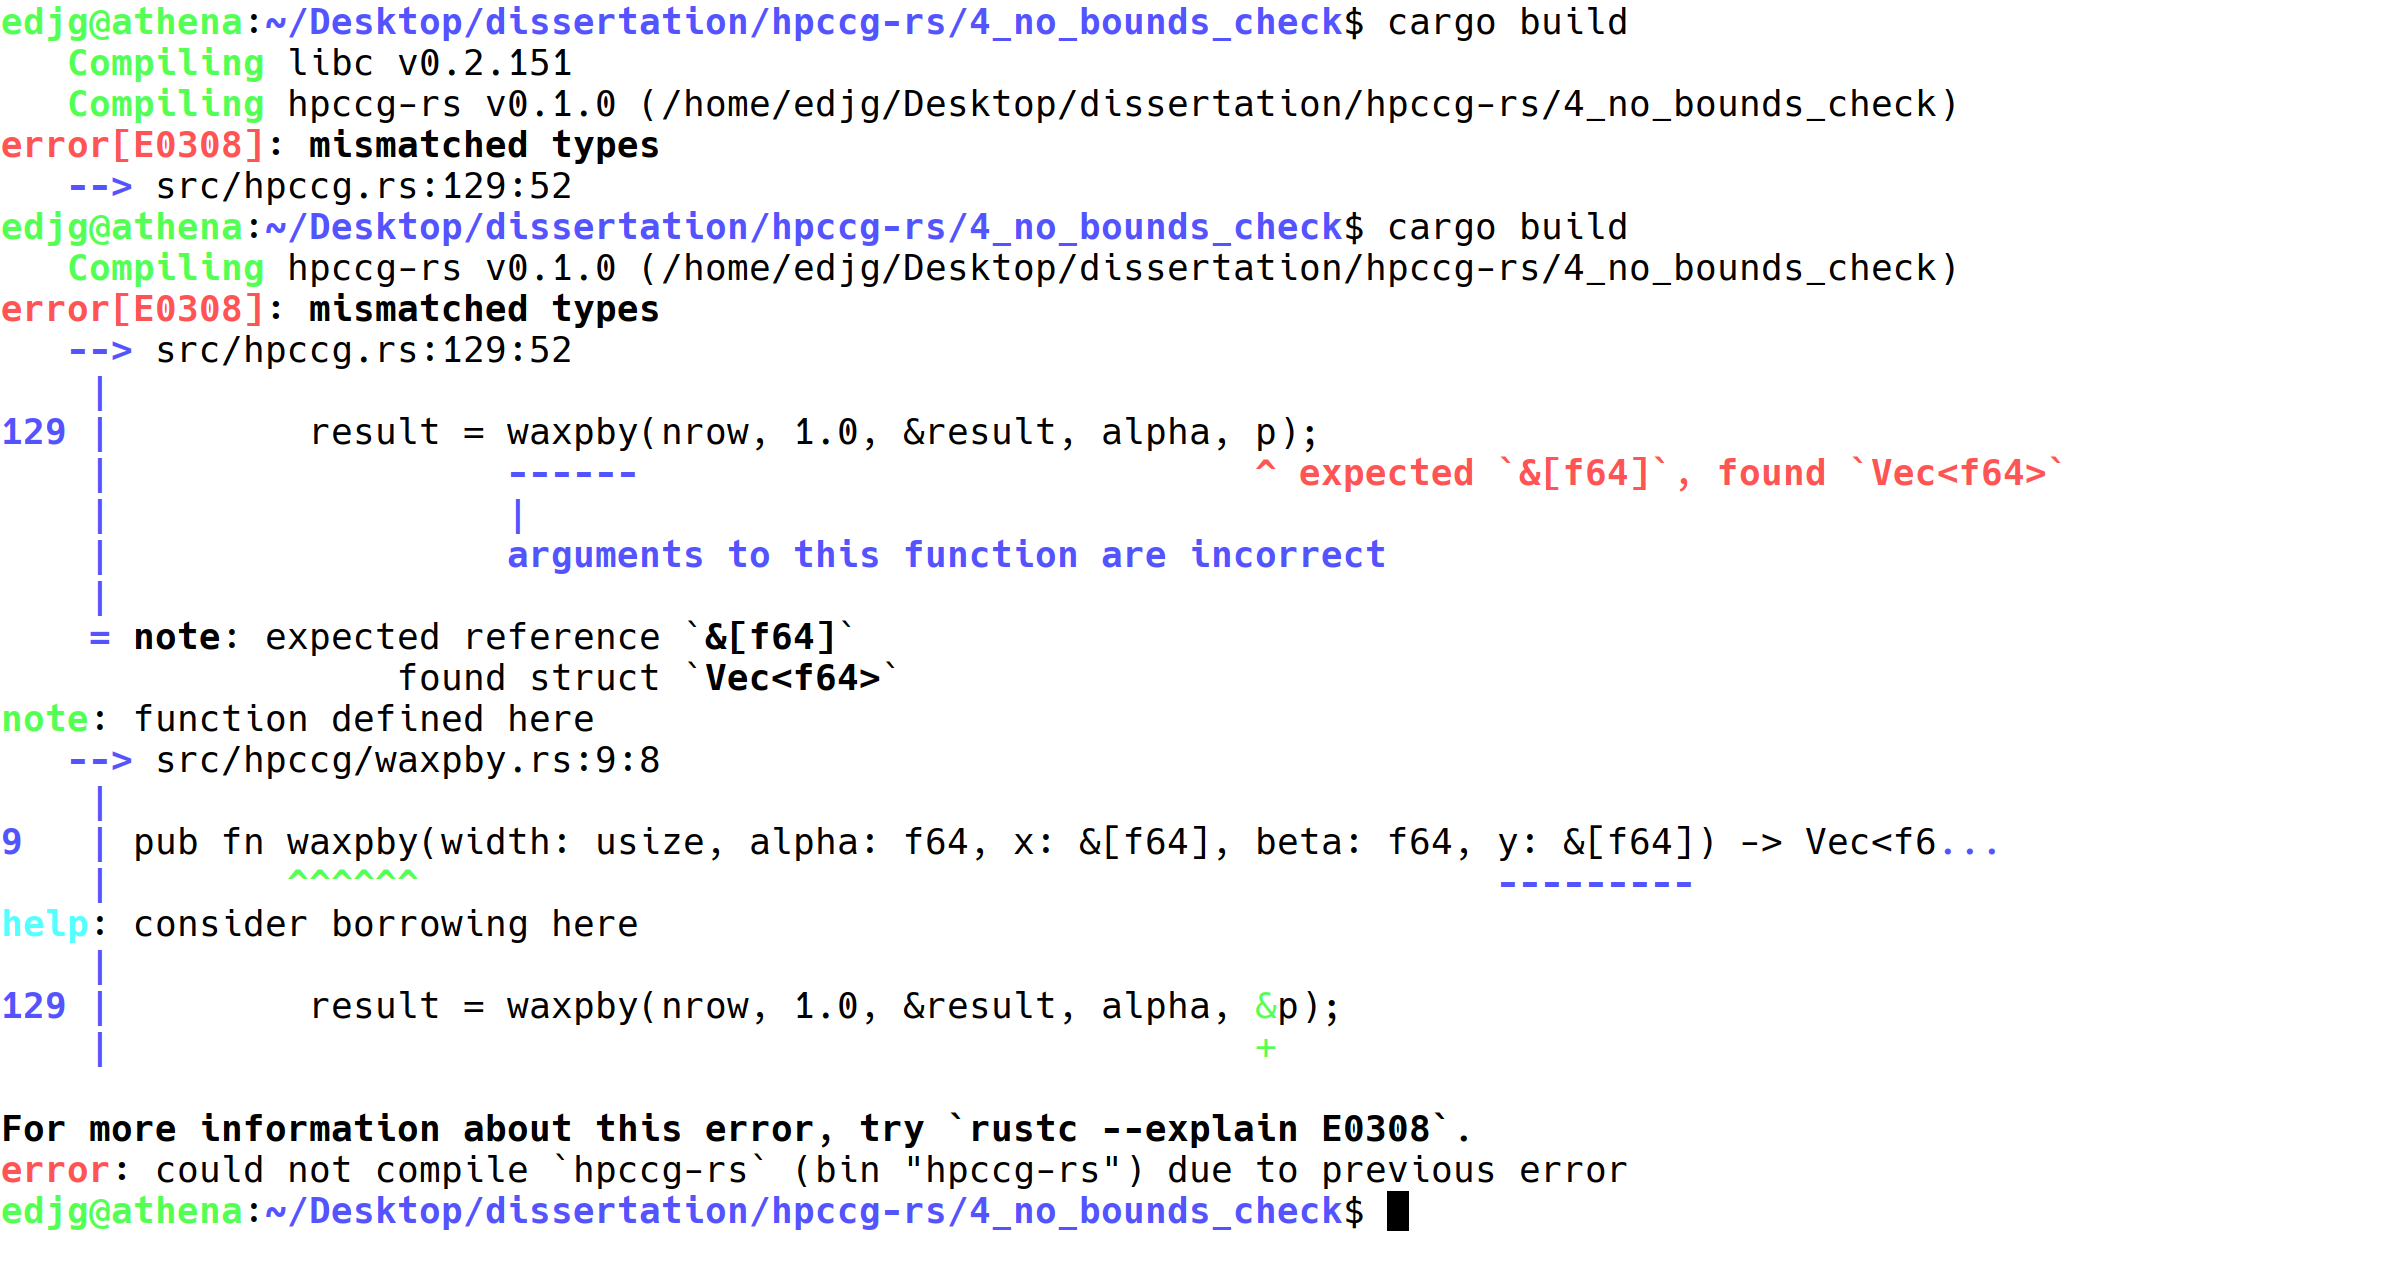
\includegraphics[width=0.95\textwidth]{images/2_background/rust_error_messages.png}
    \caption{Example of an error message, including a correct suggestion to fix it, generated by Rust as a result of a missing \mintinline{rust}{&} required to borrow the value.}
    \label{fig:rust_error_messages}
\end{figure}

On top of this, Rust provides a canonical auto-formatter called \texttt{rustfmt} \cite{RustlangRustfmt2024}, and a linter called \texttt{clippy} \cite{RustlangRustclippy2024}, which are a key component of modern development best practices. This contrasts C++, where various different, often contradictory lint and auto-format standards exist. This means that developers have to make the decision to pick one, rather than just using the canonical one. Finally, Rust provides a package manager called \texttt{cargo} \cite{RustlangCargo2024}, and a package repository called \textit{crates.io} \cite{CratesIoRust}. These allow the Rust community to share packages,
%referred to as crates, % These are not technically the same thing
to extend the functionality of Rust beyond the base language. As a result of this, despite its comparatively young age, Rust has a thriving ecosystem of packages for many tasks. This again contrasts C++, which does not have a canonical package manager, with programmers being split across \texttt{conan} \cite{ConanioConan2024}, \texttt{vcpkg} \cite{MicrosoftVcpkg2024}, domain-specific tools like \texttt{spack} \cite{gamblin2015spack}, and manual installation through header files, causing fragmentation of the package ecosystem.

\subsection{Widespread adoption}
\label{ssec:rust-adoption}

Efforts to adopt Rust in security sensitive parts of existing products, such as parsers for untrusted inputs \cite{OxidationMozillaWiki}, have existed for many years. For example, the first production code example of Mozilla's Oxidation effort to ``integrat[e] Rust code in and around Firefox'' was a MP4 metadata parser in Firefox 48 \cite{OxidationMozillaWiki}, released in 2016. However, in recent years these efforts have become far more widespread, for example Google introducing first-class Rust support for Android development in 2021, motivated by its memory safe properties \cite{RustAndroidPlatform}.

Even in the past two months at the time of writing, there have been widely reported moves towards Rust adoption. Firstly, the White House Office of the National Cyber Director publishing a press release ``Future Software Should Be Memory Safe'', encouraging developers to adopt memory safe languages, such as Rust for systems programming applications, to ``to reduce the attack surface in cyberspace'' as a matter of national security \cite{PressReleaseFuture2024}. In addition to this, Google pledged one million dollars to improve Rust's interoperability with C++, including through tooling such as \texttt{autocxx} \cite{GoogleAutocxx2024} and \texttt{bindgen} \cite{RustlangRustbindgen2024}. In the course of this project, the author made an open source contribution to \texttt{autocxx} to unblock an issue around the use of arrays \cite{goodmanAddIntegrationTests}, a common task in \acrshort{HPC}. This is discussed in more detail in section \ref{sec:open-source-work}.






\section{High performance computing}
\label{sec:hpc}

This background to \acrshort{HPC} will address recent trends in hardware design, and how they impact modern approaches to writing highly performant software. It will then address the Mantevo project, giving a brief history and linking its motivation to software approaches. Finally, it will discuss HPCCG, a \acrshort{mini-app} in the Mantevo project, and the target of the translation effort in this project.

\subsection{Recent trends in hardware design}
\label{ssec:hardware-design-trends}

In the early 2010s, physical limitations began to change how computer hardware was designed. Before this point, performance gains in hardware could be guaranteed by increasing clock speeds. However, as shown in Figure \ref{fig:scaling-trends-transistor-clock}, power limitations heralded the so-called ``death of CPU frequency scaling'', marked by Intel's cancellation of the 4GHz CPU project in 2004 \cite{markovLimitsFundamentalLimits2014}.

% TODO: Check rules about replicating diagrams from paper with correct attribution
\begin{figure}[H]
    \centering
    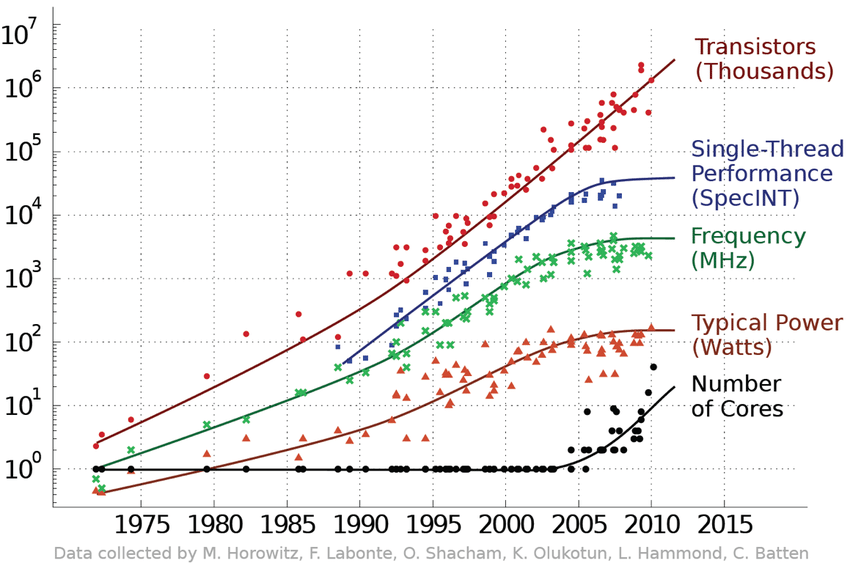
\includegraphics[width=0.75\textwidth]{images/2_background/1-Trends-in-transistor-count-performance-core-count-and-power-over-the-past-decades.png}
    \caption{``Trends in transistor count, performance, core count and power over the past decades'', reproduced from Chao Chen's ``Energy-efficient electrical and silicon-photonic networks in manycore systems'' \cite{chenEnergyefficientElectricalSiliconphotonic2014}.}
    \label{fig:scaling-trends-transistor-clock}
\end{figure}

As a result of this, the 2013 Mantevo paper notes that ``future performance gains come almost solely from running sets of instructions concurrently'' \cite{heroux2013mantevo}. This can be seen in Figure \ref{fig:scaling-trends-transistor-clock} as the increase in prevalence of multicore processors for parallel execution. There are some mechanisms which allow this to be implemented transparently to the programmer in hardware, such as instruction-level parallelism through superscalar processing and out-of-order execution \cite{pattersonHennessyComputerOrganisationArchitecture}, or vectorisation for SIMD processing \cite{pattersonHennessyComputerOrganisationArchitecture}. However, these performance gains begin to be curtailed by data hazards inherent to the software being executed \cite{shahhoseini1999achieving}, along with physical limitations to silicon footprint for a single CPU. As a result of this, parallelism approaches which are not transparent to the programmer are required for further performance increases.

\subsection{Shared memory parallelism}
\label{ssec:shared-memory-paralellism}

Shared memory parallelism refers to dividing work between multiple threads or processes, which all have access to a common memory architecture \cite{SharedMemoryParallelism}. Threads can be defined as ``basic units to which the operating system allocates processor time'' \cite{karl-bridge-microsoftProcessesThreadsWin322021}. In machines with multiple processors in a shared memory architecture, multiple threads can be executed in parallel. When the number of threads exceeds the number of logical processors, the operating system scheduler will interleave the threads to allow concurrent execution. Programs running workloads in parallel on a single machine typically use multiple threads to achieve this parallel execution. Multi-threading for shared memory parallelism can be implemented manually using thread and synchronisation primitives, such as those provided by \texttt{pthread} \cite{nichols1996pthreads}. However, frameworks such as OpenMP \cite{dagumOpenMPIndustryStandard1998} provide a convenient API for writing parallel programs, including compiler directives for FORTRAN and C/C++ which facilitate adding shared memory parallelism to code.

The OpenMP API is designed to make it easy for programmers to leverage parallelism in common programming scenarios, such as iteration. Listings \ref{listing:cpp-ddot}, \ref{listing:cpp-ddot-openmp-race}, and \ref{listing:cpp-ddot-openmp-reduction} provide a simple example of an application of OpenMP to parallelise an implementation of the dot product operation.

\begin{code}
    %TC:ignore
    \begin{minted}{c++}
        double dot_product (
            int n, double* x, double* y
        ) {
            double result = 0.0;
            for (int i = 0; i < n; i++) {
                result += x[i] * y[i];
            }
            return result;
        }
    \end{minted}
    %TC:endignore
    \caption{C++ function implementing the dot product operation on two arrays.}
    \label{listing:cpp-ddot}
\end{code}

\begin{code}
    %TC:ignore
    \begin{minted}{c++}
        double dot_product (
            int n, double* x, double* y
        ) {
            double result = 0.0;
        #pragma omp parallel for
            for (int i = 0; i < n; i++) {
                result += x[i] * y[i];
            }
            return result;
        }
    \end{minted}
    %TC:endignore
    \caption{C++ function using OpenMP to parallelise the dot product operation, containing a race condition.}
    \label{listing:cpp-ddot-openmp-race}
\end{code}

In Figure \ref{listing:cpp-ddot-openmp-race}, we can see the application of the OpenMP pragma \mintinline[breaklines]{c++}{#pragma omp parallel for} on line 5. This demonstrates how intuitive and readable the OpenMP API is, achieving in one line what would take many lines of code to manually implement using \texttt{pthread} primitives. However, Listing \ref{listing:cpp-ddot-openmp-race} contains a data race. On line 7, multiple threads may concurrently increment the result, which is not an atomic operation. This may lead to the program missing array cells from the sum, making the result unreliable.

\begin{code}
    %TC:ignore
    \begin{minted}{c++}
        double dot_product (
            int n, double* x, double* y
        ) {
            double result = 0.0;
        #pragma omp parallel for reduction(+:result)
            for (int i = 0; i < n; i++) {
                result += x[i] * y[i];
            }
            return result;
        }
    \end{minted}
    %TC:endignore
    \caption{C++ function using OpenMP to parallelise the dot product operation, using a reduction to avoid a race condition.}
    \label{listing:cpp-ddot-openmp-reduction}
\end{code}

Listing \ref{listing:cpp-ddot-openmp-reduction} shows how this can be simply mitigated by using an OpenMP reduction, which avoids this issue by maintaining local copies of the result across threads, then combining them at the end. However, this shows how susceptible even simple parallel programs can be to errors which are difficult to debug. As discussed in section \ref{ssec:rust-fearless-concurrency}, Rust provides guarantees against this category of undefined behaviour, motivating its use in \acrshort{HPC} applications, which often rely heavily on multi-threading.

The multi-threading approach to parallel is very effective for single machines running small or medium-sized programs. However, it is dependent on the machine it is executing having a shared memory architecture, so cannot scale beyond running on a single machine to clusters of computers. As a result of this, different approaches are required to aggregate together the work done by machines within a compute cluster with a distributed memory architecture.

\subsection{Distributed memory parallelism}
\label{ssec:distributed-memory-paralellism}

Distributed memory parallelism refers to dividing work across ``a computing system in which each processor has its memory'' \cite{pardo2021modeling}. A common approach to implement this is a message passing across a high-speed network connection. MPI, an initialism for Message Passing Interface, is a standard first proposed in 1993 which defined a communication protocol for exchanging data between ``MIMD distributed memory concurrent computers'' \cite{thempiforumMPIMessagePassing1993}. Two pieces of key terminology in MPI are ``rank'' and ``size''. Size refers to the number of distributed processors being used to execute the program, and rank the unique index of the processor an instance of code is executing on -- bounded between $0$ and $size-1$. MPI allows the concurrent execution of programs across many distributed processors, with each individual program rank running independently, but able to communicate with other ranks via message passing.

There are multiple implementations of the MPI standard, such as OpenMPI \cite{gabriel2004open} and MPICH \cite{gropp1996user}. These provide the functionality defined by the MPI standard for languages such as C++, FORTRAN, and Java. The MPI API is more complex than OpenMP, without the convenient compiler directives for parallelising loops, instead requiring more manual control over the way in which work is distributed. However, this provides the commensurate benefit of the ability to precisely control how data is shared, and allows it to operate over a distributed memory architecture.

Again taking the example of the dot product operation shown in Listing \ref{listing:cpp-ddot}, Listing \ref{listing:cpp-ddot-mpi} shows how MPI can be used to distribute the operation across a many ranks, allowing it to leverage parallelism on a distributed memory architecture.

\begin{code}
    %TC:ignore
    \begin{minted}{c++}
        #include <mpi.h>
        
        double dot_product (
            int n, double* x, double* y
        ) {
            // Manually split the array across the ranks
            int size, rank;
            MPI_Comm_size(MPI_COMM_WORLD, &size);
            MPI_Comm_rank(MPI_COMM_WORLD, &rank);
            int offset = ((n / size) * rank);
            int length = (rank != size - 1) ? length / size : length - offset;
        
            // Calculate the dot product for the rank's array slice
            double local_result = 0.0;
            for (int i = offset; i < offset + length; i++) {
                local_result += x[i] * y[i];
            }
        
            // Reduce the result across all the ranks
            double result = 0.0;
            MPI_Allreduce(&local_result, &result, 1, MPI_DOUBLE, MPI_SUM, MPI_COMM_WORLD);
            return result;
        }
    \end{minted}
    %TC:endignore
    \caption{C++ function using MPI to parallelise the dot product operation.}
    \label{listing:cpp-ddot-mpi}
\end{code}

Even in this simple code snippet, we can see the additional programmer effort required to use MPI over OpenMP. Lines 6 to 11 of Listing \ref{listing:cpp-ddot-mpi} manually split up the array to the ranks, whereas the OpenMP compiler directive does this automatically. The \mintinline{rust}{MPI_Allreduce} command on line 21 sends messages containing the local result to be reduced together with the \mintinline{rust}{MPI_SUM} operation to calculate the global result, which is the transmitted back as a message to all the ranks.

\subsection{Performance portability frameworks}
\label{ssec:performance-portability-frameworks}

There also exist portability frameworks, such as Kokkos \cite{edwardsKokkosEnablingPerformance2013} and RAJA \cite{RAJAPortabilitySuite}, which provide an abstraction over many parallelism techniques to improve software portability. This reduces the programmer effort to write software which is highly performant across different hardware, but can incur a performance cost. As with OpenMP and MPI, taking the example of the dot product operation shown in Listing \ref{listing:cpp-ddot}, an implementation of the same function using Kokkos for parallel execution is shown in Listing \ref{listing:cpp-ddot-kokkos}.

\begin{code}
    %TC:ignore
    \begin{minted}{c++}
        #include <Kokkos_Core.hpp>
        
        double dot_product (
            int n, double* x, double* y
        ) {
            double result = 0.0;
            Kokkos::parallel_reduce(
                n,
                KOKKOS_LAMBDA(const int i, double& ksum) {
                     ksum += x[i] * y[i];
                },
                result
            );
            return result;
        }
    \end{minted}
    %TC:endignore
    \caption{C++ function using OpenMP to parallelise the dot product operation, using a reduction to avoid a race condition.}
    \label{listing:cpp-ddot-kokkos}
\end{code}

Kokkos is designed to be ``hardware agnostic'', providing an abstraction for writing performant code which can run on across CPUs and GPUs from a variety of hardware vendors \cite{KokkosEcosystem}. As discussed in the later section \ref{ssec:p3hpc}, this provides both productivity and portability for the programmer, as this abstraction means they can be less concerned about compatibility across hardware. However, this can come at a performance cost, as the abstraction may not be able to compile to be as performant as hand-optimised code. The prominence of Kokkos in the \acrshort{HPC} space is encouraging for the suitability of Rust for the same space, as it means that programmers are willing to make sacrifices in performance for commensurate improvements to other aspects of software development, such as productivity and portability.

Since these mechanisms to leverage hardware for performance improvements are not transparent to the programmer, hardware-software co-design, defined by the 2013 Mantevo paper as ``collaborative simultaneous development of all system components'' \cite{heroux2013mantevo} became essential. As a result of this, new techniques were required for the effective co-design of high-performance systems.

\subsection{Mini-apps and the Mantevo Suite}
\label{ssec:miniapps-mantevo}

The Mantevo project at Sandia National Labs pioneered the concept of \acrshort{mini-app}s as a tool for hardware-software co-design, publishing the Mantevo Suite in late 2012 as a collection of full-featured \acrshort{mini-app}s for this purpose. It defines \acrshort{mini-app}s as ``Small software programs [...] whose performance characteristics model full-scale applications, yet require only a fraction of the lines of code, making [them] easier to study, design, and re-write'' \cite{heroux2013mantevo}.

The use of \acrshort{mini-app}s makes hardware-software co-design for large, complex applications possible. This is because they can be used in place of the production application whose performance they model when making very early design decisions, without incurring the cost of massive complexity of the production application. Traditionally, \acrshort{mini-app}s have been used to predict the performance of production applications on new hardware. However, this concept can be inverted to instead use \acrshort{mini-app}s to predict the performance on the underlying software stack, for example the programming language of implementation.

\subsection{HPCCG}
\label{ssec:hpccg}

HPCCG is an initialism for ``High Performance Computing Conjugate Gradients'', and is ``the original Mantevo mini-app'' \cite{herouxHPCCGSolverPackage2007}. It is designed to be ``the best approximation to an unstructured implicit finite element or finite volume application in 800 lines or fewer.'' \cite{PackagesMantevo}. This short length, along with its simple build system, and support for OpenMP and MPI with no other dependencies made it a good choice for translation to Rust. A full description of the process leading to the selection of HPCCG is described in Appendix \ref{sec:miniapp-selection}.

It is based on the iterative method of gradient descent for conjugate gradients first proposed by Hestnes and Steifel in 1952\cite{hestenesMethodsConjugateGradients1952}, who researched it and wrote an implementation for the contemporary Z4 processor. This process can be used to model, and hence visualise, pressure dissipation over time in a three-dimensional mesh as shown in Figure \ref{fig:acacgs_silo_output}.

\begin{figure}[H]
    \centering
    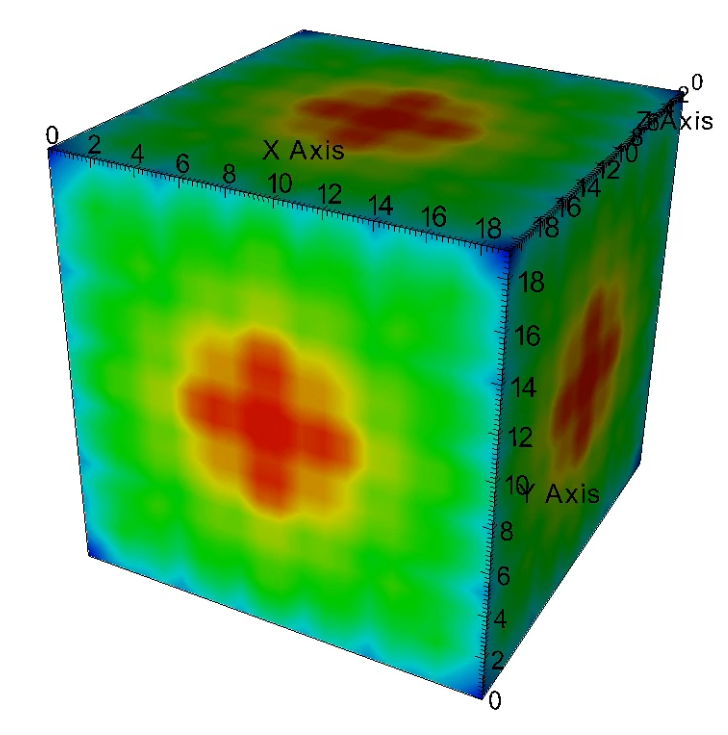
\includegraphics[width=0.5\textwidth]{images/2_background/acacgs_silo_output.png}
    \caption{VisIt visualisation from ACACGS, a C translation of HPCCG by Dr Richard Kirk which is used in the CS257 Advanced Computer Architecture coursework.}
    \label{fig:acacgs_silo_output}
\end{figure}

There are three main operations in this iterative method of conjugate gradients: calculating a vector dot product, pairwise summation of two scaled vectors, and calculating the product of a sparse matrix and a vector. Of the three operations, the third operation is responsible for most of the floating point operations, and consequently the majority of the runtime. This is because calculating sparse matrix-vector products requires larger and more complex data structures to efficiently represent sparse matrices, rather than just vectors.

Sparse matrix-vector products are a common workload in \acrshort{HPC}, and remain an active field of research, with Lane and Booth describing them as ``one of the most important kernels in high-performance computing'' \cite{laneHeterogeneousSparseMatrixVector2023}. This means that the performance characteristics of HPCCG, which are dominated by this kernel, are representative of many large applications. Since sparse matrices are ubiquitous in computational tasks, there are well-established data structures to represent them. One of these representations is compressed row storage, often called Yale format, as it was first proposed in the 1977 Yale Sparse Matrix Package report \cite{eisenstat1977yale}.

\subsection{Performance, Productivity, and Portability}
\label{ssec:p3hpc}

In the real world, \acrshort{HPC} projects are constrained by budget. Since supercomputers are extraordinarily expensive, it is easy to assume that the dominant effect on project cost is performance, as more performant software requires less time on the supercomputer, which costs money. However, other aspects of software engineering also impact the calculus of the cost of \acrshort{HPC} projects. Engineers are required to build software and maintain the servers for the project, and high-quality engineers capable of undertaking such tasks require high salaries. As a result of this, productivity and portability play a significant role in project cost, as well as raw performance. This fact is confirmed by the existence of the P3HPC conference, standing for ``Performance, Portability, and Productivity in HPC'', which focusses on ``research that addresses the complexities of real-life applications and/or realistic workloads'' \cite{P3HPC}.

% NOTE: THIS IS A KEY PARAGRAPH! IS IT PROMINENT ENOUGH?
Developer productivity plays a key role in \acrshort{HPC} projects. This is because is more productive developers will complete tasks more quickly, so fewer developer hours are required per project. In addition to this, projects with the same number of developers will be completed faster if the developers are more productive. In real projects constrained by budget, these are both clearly desirable outcomes. As a result of this, workflows and methodologies which can augment developer productivity are very beneficial within \acrshort{HPC}. Rust's guarantees of memory and thread safety, its terse syntax, and robust development toolchain all contribute to developer productivity, with fewer lines of code required to express the same functionality, and less time spent debugging.

Portability across hardware architectures is also a key consideration when building software for \acrshort{HPC} systems. Supercomputers are not homogeneous in architecture, with Intel, AMD, and Cray all being common platforms. Performance characteristics of software across architectures are difficult to predict, with architectural choices such as cache size deeply impacting performance of certain workloads. As a result of this, techniques to build software which is portable across many systems are very desirable.

% NOTE: Is this consistent tense?
As a result of this, this project will take a holistic view of software development for \acrshort{HPC}, assessing not only the raw performance of Rust, but also taking into context its effects on developer productivity, and its portability across different hardware architectures. In addition to this, developer tooling will be built to enhance the productivity of engineers in aspects of the translation workflow identified as viable for augmentation by tooling.


\section{Literature review}
\label{sec:literature-review}

Rust's popularity has led to academic investigations of its suitability for many tasks, despite it being a relatively young language. This literature review will start with a paper discussing the overall landscape of language performance for \acrshort{HPC}, comparing a single workload across 10 languages. Then, it will critically evaluate a number of performance analyses of Rust in \acrshort{HPC}, in order to cover a variety of techniques, from serial to highly parallel, and a variety of benchmark types, from algorithm snippets to full codebases. This project differs from existing work, as no existing analysis covers the implementation of an established \acrshort{mini-app} to highly-parallel clustered compute, and it will include an assessment of practical suitability beyond just performance measurements. Furthermore, it will go beyond comparison to build tooling and workflows to directly improve any issues identified during this assessment.

\subsection{Benchmarking the Parallel 1D Heat Equation Solver}
\label{ssec:diehl-et-al}

% Benchmarking the Parallel 1D Heat Equation Solver in Chapel, Charm++, C++, HPX, Go, Julia, Python, Rust, Swift, and Java
% https://github.com/diehlpk/async_heat_equation/tree/main
Diehl et al. present a general overview of the landscape of language performance for a representative \acrshort{HPC} workload in their paper ``Benchmarking the Parallel 1D Heat Equation Solver in Chapel, Charm++, C++, HPX, Go, Julia, Python, Rust, Swift, and Java'' \cite{diehlBenchmarkingParallel1D2023}. This paper selects a 1D heat diffusion solver algorithm to implement, as it uses block-structured meshes, which are commonly used in \acrshort{HPC} applications. It then goes on to qualitatively discuss the experience of implementing the algorithm in the different languages, and suggests a quantitative metric for assessing implementation difficulty, the \acrfull{COCOMO} \cite{boehm1995cost}. Finally, it benchmarks these implementations across three different hardware architectures, and constructs a plot comparing program runtime against its metric for implementation difficulty, duplicated in Figure \ref{fig:1d_heat_results}. The paper concludes that ``one solution does not fit all'', but names C++ as a common choice as it is both popular and performant, whilst noting Rust's ``innovative ideas will make it ideally suited for many applications''.

\begin{figure}[H]
    \centering
    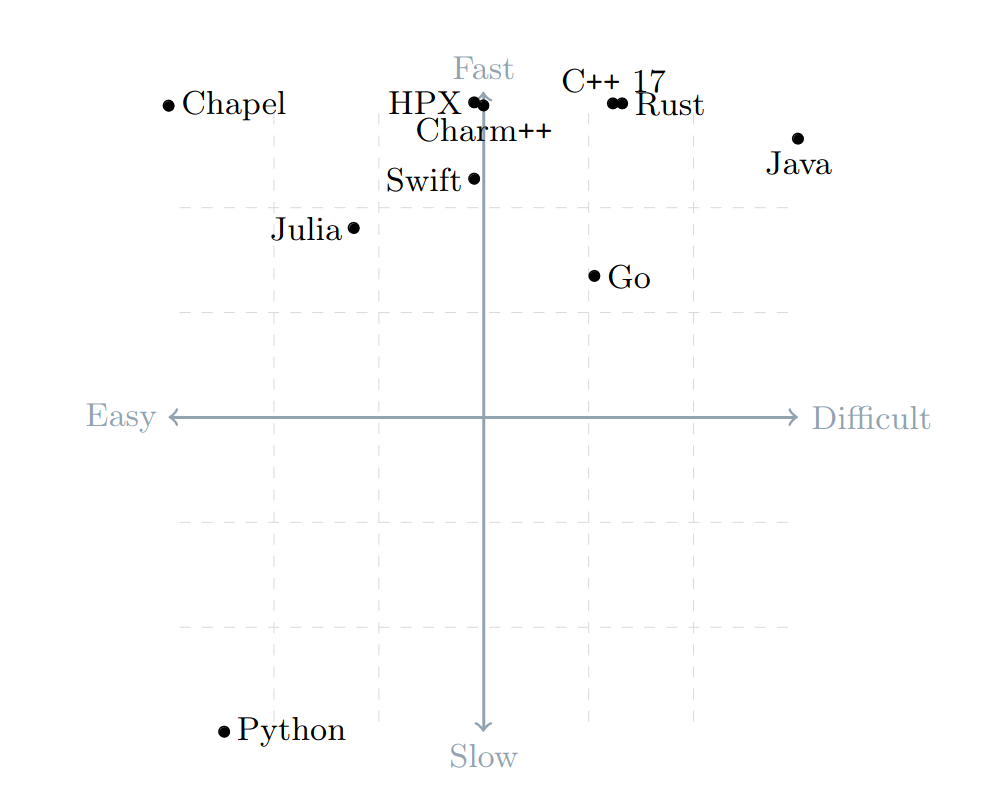
\includegraphics[width=0.75\textwidth]{images/2_background/1d_heat_results.png}
    \caption{``Two-dimensional classification using the computational time and the \acrshort{COCOMO} model [sic]'', reproduced from Diehl et al.'s paper \cite{diehlBenchmarkingParallel1D2023}.}
    \label{fig:1d_heat_results}
    % TODO: Check paper website for permission to reproduce
\end{figure}

Diehl et al. provide a strong empirical analysis of the landscape of languages in the context of \acrshort{HPC}, and provide source code as a GitHub repository \cite{diehlInitialRelease2023} along with naming the multiple processors used for benchmarking, allowing reproducibility of their results. However, they explicitly do not provide their measurements other than in plots, choosing ``not to name a winner with respect to speed''. Additionally, they do not provide details on their test methodology beyond naming the metrics measured and the names of hardware they used. Providing concrete results, along with a more specific methodology such as thread counts, memory size, or number of experiment re-runs would provide much more confidence in the conclusions drawn. Finally, their future work notes that the selected algorithm only runs on a single CPU, and as such does not explore using MPI for distributing compute over a clustered resource, nor does it explore GPU support using a language like CUDA, nor abstractions layers like Kokkos.

\subsection{Rust language for supercomputing applications}
\label{ssec:bychkov-nikolskiy}

% Rust language for supercomputing applications
% Serial, parallel, and MPI - but on non-standard small code snippet benchmarks. Present but flawed methodology.
Bychkov and Nikolskiy examine the readiness of the Rust language for supercomputer applications in their paper ``Rust Language for Supercomputing Applications'' \cite{bychkovRustLanguageSupercomputing2021}. The main contribution of this paper is the critical comparison of Rust and C++ over a set of benchmarks. The first benchmark characterises serial performance via a handwritten implementation of the matrix multiplication algorithm in each language. The authors note that naive rust implementations perform poorly in comparison with C++, but writing idiomatic Rust and leveraging optimisation techniques can close this performance gap. A later benchmark characterises the performance of shared-memory parallelism via multi-threading, using OpenMP and \texttt{rayon} for C++ and Rust respectively, finding that both have similar performance and scaling characteristics on the selected benchmark. The final benchmark compares the C++ native implementation of the MPI specification with the Rust bindings to it. The paper notes that since the Rust bindings are memory safe and leverage the rich type system, they provide many desirable properties such as guarantees of memory and thread safety and minimising boilerplate. The paper concludes that Rust is competitive to C++ for the benchmarks it explored, and that there is sufficient support for writing parallel code.

Bychkov and Nikolskiy present an empirical analysis directly comparing Rust and C++ only across a number of different benchmarks, contrasting Diehl et al. by providing a more specific analysis rather than a general view of the landscape. The paper gives fair reproducibility of results by clearly stating the benchmarking methodology, including machine specifications, operating system, and compiler versions. However, the choice of methodology for non-clustered machines has weaknesses. Notably, the benchmarks were run on a laptop, which can introduce noise into performance measurements if other applications are running in the background. Furthermore, the benchmarks are run under Windows Subsystem for Linux, a virtualisation technology, which significantly impacts program performance and may not be comparable to benchmarks run on unvirtualised systems. Finally, although the MPI benchmarks are run on a compute cluster which avoids the previously itemised issues, the results appear erroneous, with the authors noting ``we discovered [an] unexpected difference between Rust and C++ performance in MPI latency benchmarks'', and stating intent to re-validate the results.

% If needed, perhaps later... Higher quality paper than Bychkov and Nikolskiy, so consider replacing
% Rust programming language in the high-performance computing environment
% Rayon + MPI implementation of code snippet, run data but no source code

\subsection{Performance vs Programming Effort between Rust and C on Multicore Architectures}
\label{ssec:costanzo-et-al}

% Performance vs Programming Effort between Rust and C on Multicore Architectures: Case Study in N-Body
% https://github.com/ManuelCostanzo/Gravitational_N_Bodies_Rust (250 lines of rust)
Costanzo et al. investigate the difference between both performance and programming effort between Rust and C for N-body simulations in their paper ``Performance vs Programming Effort between Rust and C on Multicore Architectures: Case Study in N-Body'' \cite{costanzoPerformanceVsProgramming2021}. The paper introduces Rust as a programming language which may be suitable for \acrshort{HPC} due to its ownership model avoiding the need for garbage collection, and its strong support for shared-memory parallelism. It then discusses the implementation and performance optimisation of C and Rust to the gravitational n-body problem, a simple and well-known computational task. It finally compares the both the performance and programming effort of the C and Rust implementations. The paper concludes that Rust is either equally performant or slightly ($1.18\times$) slower depending on the data type precision, but that this may change with future compiler updates, and Rust requires a lower programming both in terms of lines of code and ease of parallelisation.

Costanzo et al. provide a very compelling empirical analysis comparing Rust and C++, which differs from Bychkov and Nikolskiy by considering both the practical implications of programming effort, and making the comparison on a representative code sample rather than simple benchmarks. However, the paper does not consider highly-parallel clustered compute using technologies such as MPI. The paper provides a discussion of practical techniques for writing performant Rust beyond threading, including use of SIMD intrinsics and custom memory allocators, along with a compelling and unbiased performance analysis of Rust and C++.


\subsection{Emerging technologies, Rust in HPC}
\label{ssec:moran-bull}

% Emerging technologies, Rust in HPC
% Parallel only implementation for non-standard very small full application for C++ and Fortran, good methodology. Poor Rust implementation
% https://github.com/lmoran94/eurocc_cfd (112 lines of Rust)
Moran and Bull \cite{moranEmergingTechnologiesRust2023} investigate the performance of Rust as compared with C++ and FORTRAN on computational fluid dynamics problems in their technical report ``Emerging Technologies: Rust in HPC'' \cite{moranEmergingTechnologiesRust2023}. As with Costanzo et al., Rust is introduced as a programming language which may be suitable for HPC, and the selected problem domain is explained as representative of common \acrshort{HPC} workloads. The paper goes on to benchmark Rust implementations of the problem on a HPC system, and compare them to C++ and FORTRAN implementations. The paper concludes that Rust is slower than C++ and FORTRAN for parallel workloads.

Moran and Bull present a similar empirical analysis to Costanzo et al., comparing a small custom codebase which is representative of \acrshort{HPC} workloads, but differs by including FORTRAN in its comparisons, along with placing a greater focus on performance analysis and scaling, and less consideration to programming effort. However, Moran and Bull report significantly slower performance, significantly trailing C++ and FORTRAN, which contrasts Costanzo et al.'s findings of Rust being slightly slower or equally performant. Moran and Bull attribute their findings to the Rust compiler's attitude to memory safety.

However, inspecting the source code made public after the publication of the paper \cite{Lmoran94Eurocc_cfdCFD}, it can be seen that the implementation does not leverage all the performance capabilities of Rust. For example, it does not apply all of the optimisation techniques enumerated in Costanzo et al.'s paper. A reader of the paper created an optimised version  \cite{moranPaperFalse} \cite{phazer99HerePlayground2023}, which shows a 50\% performance increase over the paper's implementation by avoiding an extraneous copy operation, bringing Rust's performance closer to C++ and FORTRAN. However, this change makes the comparison against FORTRAN and C++ unfair, as the reference implementations also rely on this extraneous copy operation. A replication trial of the experiments in the paper using the published code is presented in section \ref{ssec:hpc-multibench-replication-study}, as both a demonstration of the utility of the HPC MultiBench tool, and to investigate the difference to Costanzo et al.'s findings.
% In summary, possibly flawed due to bounds checked memory access, but not as flawed as some commentators looking only at the Rust implementation think it is.


% % Towards Safe HPC: Productivity and Performance via Rust Interfaces for a Distributed C++ Actors Library
% % This could be omitted, as they paper is a ``work in progress'' and clearly flawed, and other more interesting papers exist...
% Parrish et al. present a framework for writing parallel programs, including a performance analysis of this framework, in their paper ``Towards Safe HPC: Productivity and Performance via Rust Interfaces for a Distributed C++ Actors Library (Work in Progress) [sic]'' \cite{parrishSafeHPCProductivity2023}. The paper concludes that their ``Rust versions of the original application performed on par with the respective C++ versions''. To support this claim, the paper includes figures showing the performance of Rust and C++ for various kernels, such as the one shown replicated in Figure \ref{fig:actors_bad_histogram}.

% \begin{figure}[H]
%     \centering
%     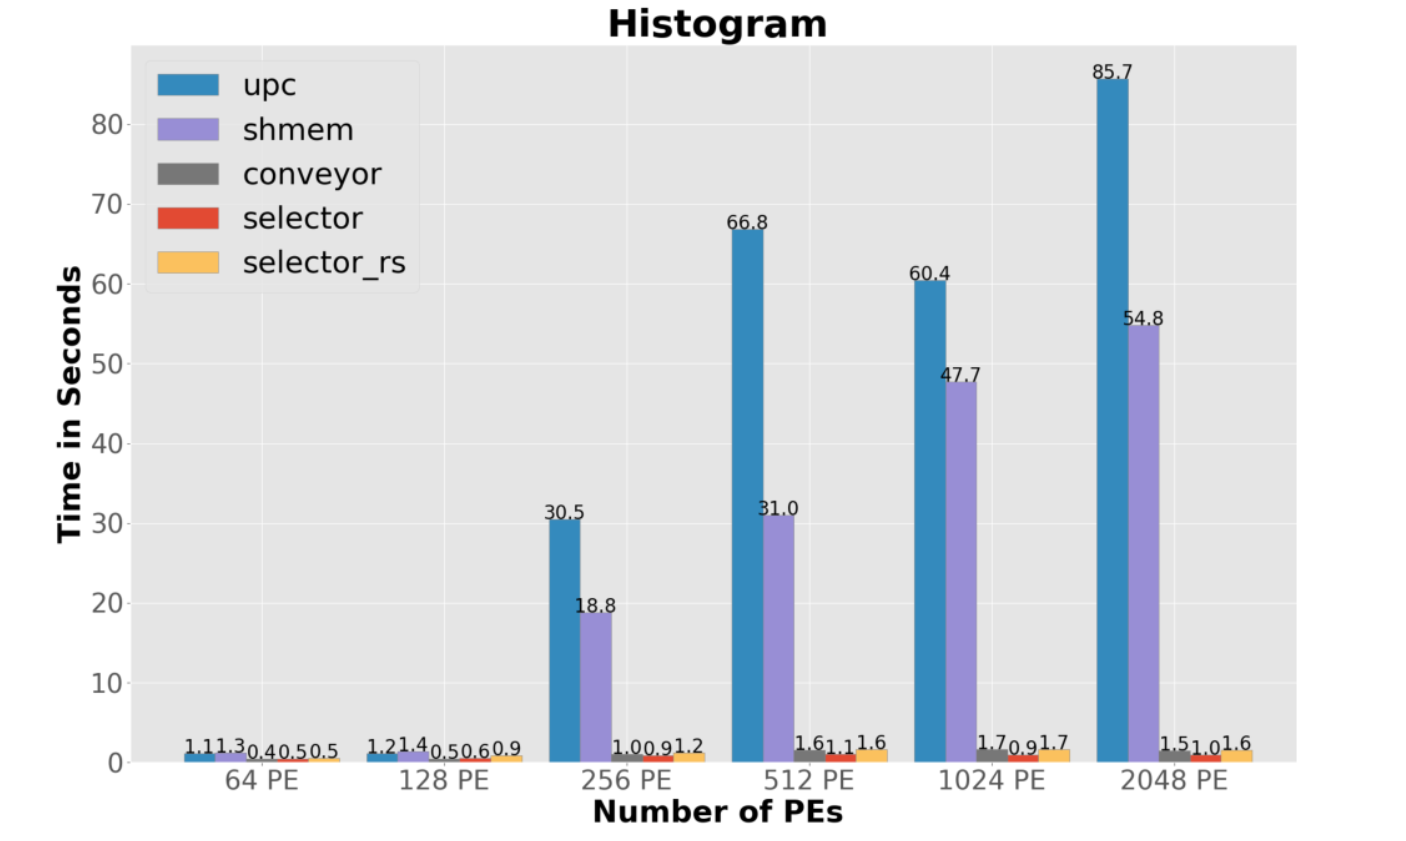
\includegraphics[width=0.75\textwidth]{images/2_background/actors_bad_histogram.png}
%     \caption{The performance of the Histogram kernel across various implementations, reproduced from Appendix A of Parrish et al. \cite{parrishSafeHPCProductivity2023}.}
%     \label{fig:actors_bad_histogram}
%     % TODO: Check paper website for permission to reproduce
% \end{figure}

% However, the data shown in Figure \ref{fig:actors_bad_histogram} does not support the claim that Rust is as performant as C++. The inclusion of the much slower ``upc'' and ``shmem'' implementations skew the scale of the plot so Rust and C++ versions look the same, but in fact by examining the data labels we can see the implementation is on average $1.46\times$ slower for this kernel, which is non-negligibly slower. This aligns with the results of other publications such as Costanzo et al. who observed a $1.18\times$ slowdown, and noted it as such. In the author's opinion, this paper is emblematic of a common problem in literature about the Rust programming language -- the bias held by some that the Rust programming language is better in all respects than other programming languages. Despite the fact that the data in the paper shows that the Rust implementation is slower \ref{fig:actors_bad_histogram}, the data is presented disingenuously in order to draw the conclusion that it is equally performant.

\subsection{Summary of literature}
\label{ssec:literature-summary}

% % Summary
% In summary, there is existing research around the suitability of Rust in High-Performance Computing, which broadly concludes that Rust is slightly slower than C++, but provides other benefits which might mitigate this fact. Some papers, such as Parrish et al. \cite{parrishSafeHPCProductivity2023} over-report the performance of Rust as equal to C++, in spite of the data they present to justify their conclusions. However, other papers, such as Moran and Bull \cite{moranEmergingTechnologiesRust2023}, under-report the performance of Rust as significantly slower than C++, likely due to not fully leveraging possible performance optimisations.
In summary, there is existing research around the suitability of Rust in \acrshort{HPC}, which broadly concludes that Rust is slightly slower than C++, but provides other benefits which might mitigate this. Some papers, such as Moran and Bull \cite{moranEmergingTechnologiesRust2023}, report the performance of Rust as significantly slower than C++. This could be as a result of different computation kernels being less amenable to optimisation, or the authors not fully leveraging performance optimisations possible in Rust.

The existence of publications, such as the ones reviewed above, in this area is compelling that it is a relevant and difficult question to answer. However, there is still space for novel contribution, for example by assessing highly-parallel clustered compute as applied to a standard \acrshort{mini-app}, rather than a simple benchmark or toy example. Furthermore, many existing papers do not focus on reproducibility of results, by omitting the source code, research methodology, or recorded results. Finally, none of the papers provide tooling to assist in the process of translating \acrshort{HPC} codebases, giving a further opportunity for novel contribution.

\chapter{Translation}
\label{ch:translation} % 4000-5000 words

% In this chapter, we describe the overall design of our solution to the problem identified in \Cref{ch:introduction}, building on work described in \Cref{ch:background}.
% TODO: Consider some kind of link from introduction

In this chapter, we discuss the translation process from C++ to Rust of the selected mini-app, HPCCG. First, we introduce the implementation details of HPCCG, along with the translation methodology undertaken. Then, we present a sequence of incrementally performant translations, showing how features of and packages for the Rust language can contribute to the performance of translations of C++ codebases. Next, we discuss approaches for the critical step of program equivalence checking to guarantee comparisons are fair. Finally, we conclude with a section on lessons learned from the process, and a proposed workflow for engineers translating High-Performance C++ codebases to Rust.

% Explain the goals of the effort
The overall goal of this effort is to generate a software product -- a Rust translation of the HPCCG codebase, with strong performance running in serial, and leveraging shared and distributed memory parallelism. On top of this, we propose a approaches for equivalence checking such translations, and use them to give confidence the Rust translation of HPCCG can be used for fair performance comparisons with the reference C++ version.

% Explain the difficulties of the effort
% No-one else has done a whole mini-app, just single kernels and toy examples
As discussed in \Cref{ch:background}, this translation effort is novel with respect to assessing High-Performance Computing for a number of reasons. Previous literature has translated only single computation kernels \cite{} with support for shared and distributed memory parallelism, or very short ``toy example'' applications of around only 150 lines \cite{} \cite{} with support for only shared memory parallelism. In contrast to this, HPCCG is a standard mini-app as part of the Mantevo suite, with the C++ version totalling 1524 lines and having support for both shared and distributed memory parallelism. This order of magnitude increase in codebase length over modern existing work \cite{}, along with support for distributed memory parallelism outside of single computation kernel contexts provides a valuable insight into the suitability of Rust in High-Performance Computing, but at the cost of significant developer effort as compared with existing work.

\section{Design}
\label{sec:translation-design} % 500 words

In traditional software development tasks, such as building the HPC MultiBench tool discussed in \Cref{ch:hpc-multibench}, system design is paramount to building a coherent product. However, for translation tasks the reference implementation has already been designed.


\subsection{Differences in the Rust and C++ programming models}
\label{sec:overview-hpccg}

\subsection{Overview of HPCCG}
\label{sec:overview-hpccg}
% Overview of HPCCG


\subsection{Translation methodology}
\label{sec:translation-methodology}
% Process of writing incrementally optimised translations


\section{Implementation}
\label{sec:translation-implementation} % 3000 words

This section provides a description of the technical details of the translation process. Source code for each of these translations can be found in the \texttt{hpccg-rs} GitHub repository.


\subsection{Direct translation}
\label{sec:translation-direct}
% Naive translation + explaining Rust ownership and borrowing
The first translation 


\subsection{Reworked data structure}
\label{sec:translation-reworked-data-structure}
% Restructured data structure

\subsection{Bounds checking}
\label{sec:translation-bounds-checking}
% Bounds checking

\subsection{Iterators}
\label{sec:translation-iterators}
% Iterators

\subsection{Shared memory parallelism}
\label{sec:translation-rayon}
% Shared-memory parallelism with Rayon

\subsection{Distributed memory parallelism}
\label{sec:translation-mpi}
% Distributed-memory parallelism with rs-mpi


\section{Equivalence checking}
\label{sec:equivalence-checking} % 3000 words

Equivalence checking is critical to make performance comparisons between programs fair. In order to draw conclusions about the performance of the Rust translation of HPCCG, there must be strong confidence that it provides the same functionality as the C++ version. Taking this to its logical extremes, a Rust program which immediately terminates will have a much lower total runtime than the C++ implementation of HPPCG, but it clearly would not be a fair comparison of Rust and C++. However, the usefulness of equivalence checking is not only for ensuring performance comparisons are fair. Any translation effort from existing C++ code to Rust 

As a result of this, a significant part of this project is developing techniques and workflows to equivalence check

\subsection{End-to-end testing}
\label{sec:equivalence-end-to-end}
% end-to-end testing

The simplest form of equivalence checking is end-to-end testing. This refers to running programs with the same input data, and asserting that they yield the same outputs.

\subsection{Formal methods}
\label{sec:equivalence-end-to-end}
% formal methods (and why they aren't suitable)

\subsection{Assembly and IR analysis}
\label{sec:equivalence-end-to-end}
% LLVM analysis (and why it is hard to scale)

\subsection{Unit testing}
\label{sec:equivalence-unit-testing}
% Unit testing

\subsubsection{Test driven development}
\label{sec:equivalence-tdd}

Test-driven development refers to


\subsection{A novel approach}
\label{sec:equivalence-polyglotest}
% polyglotest approach



% % TODO: Could omit this, it's an interesting aside, but if stuff needs to be cut, this is it
% \section{Supply-side verification}
% \label{sec:translation-supply-side-verification} % 500 words
% % Why is this important?
% % `cargo vet`


\section{Lessons learned and proposed workflow}
\label{sec:translation-workflow} % 3000 words
\chapter{HPC MultiBench}
\label{ch:hpc-multibench}

% =============================================================================================== %
% \textbf{This chapter is now complete - but wasn't in the first three chapter draft submission!} %
% =============================================================================================== %

% Having implemented the Rust translation of the HPCCG codebase, the next step is to characterise its performance. This is typically done by running many tests across a wide variety of configurations and problem sizes to understand how the program scales across these metrics.

HPC MultiBench is a tool to generate and run HPC batch compute jobs for performance comparison via Slurm from a convenient YAML configuration file. It can be thought of as ``a Swiss army knife for comparing programs on HPC resources''. This chapter will first discuss the motivation and use case for the tool, then go into technical detail about its design and implementation. Next, it will provide a concrete demonstration of its utility in an example use case, quickly constructing replication studies, by confirming the results of Moran and Bull's paper ``Emerging technologies: Rust in HPC'' \cite{moranEmergingTechnologiesRust2023}. Finally, the chapter will conclude with thoughts from an industry review of the tool by two PhD candidates working in the High Performance and Scientific Computing Group at Warwick.

\section{Motivations}
\label{sec:hpc-multibench-motivation}

Manually spawning and aggregating the metrics from many similar jobs with different configurations is tedious. It is a repetitive and time-consuming process, and as such discourages duplicating results for statistical confidence -- despite being susceptible to human error. However, it is a common task in workflows for designing High-Performance Computing software, as it provides critical metrics to characterise application performance.

Consider a single trial comparing the performance of two programs across eight problem sizes, with eight different thread counts per problem size. In total, this requires 128 program runs. Re-running this trial five times for statistical confidence requires 640 program runs, which is an untenably large number of jobs to dispatch manually. Currently, there are two approaches to this problem: either ignore statistical confidence and manually spawn many jobs, or create an application-specific script to submit the jobs. Both of these approaches are time-consuming, either manually submitting the jobs or writing and debugging the custom script. As a result of this, this step can form a bottleneck in certain workflows.

However, this process of running and aggregating jobs is very similar between performance trials for different programs, meaning it is possible to create a program to automate the process. This combination of being both time-consuming and amenable to automation makes it a very good candidate for building tooling to facilitate it, as it has a good ratio of being high-impact to requiring achievable programming effort.

\section{Existing tools}
\label{sec:hpc-multibench-existing-tools}

As High-Performance Computing is an active research space, there are a number of existing tools which also act as a wrapper around Slurm, as shown in Table \ref{tab:hpc-multibench-existing-tools}. However, none of these tools appear to provide first-class support for this particular use case.

% TODO: Check all tables have bold headings
% TODO: Consider citing GitHub on tool names and papers on tool descriptions?
\begin{table}[H]
    \caption{Existing tools which provide wrappers for Slurm.}
    \label{tab:hpc-multibench-existing-tools}
    \begin{tabular}{|p{0.2\linewidth}|p{0.8\linewidth}|}
    \hline
    \textbf{Tool name}  & \textbf{Tool description} \\ \hline\hline
    slurmR     & ``A lightweight wrapper for Slurm'' \cite{gvegayonJournalOpenSource}, which provides a framework to distribute computation of programs written in the R language across compute clusters, particularly in the field of biostatistics. \\ \hline
    targets    & ``A Make-like pipeline tool for statistics and data science in R'' \cite{landauTargetsPackageDynamic2021}, which orchestrates processing of programs written in R, providing caching capabilities to avoid re-running unchanged parts of the pipeline. \\ \hline
    batchtools & ``Provides an implementation of a Map-like operation to define and asynchronously execute jobs on a variety of parallel backends'' for the R programming language \cite{langBatchtoolsToolsWork2017}. \\ \hline
    ClusterMQ  & ``[An R package] to send function calls as jobs on a computing cluster with a minimal interface'' \cite{schubertClustermqEnablesEfficient2019}. \\ \hline
    \end{tabular}
\end{table}

From this table, we can see that a number of tools exist as wrappers for Slurm for scientific computing workflows. However, these tools are generally focussed on orchestrating High-Performance Computing resources to run scientific computing programs, often in the R programming language, rather than providing a mechanism to run and compare the performance of programs in arbitrary languages. Our research did not identify any existing tools which directly compete with the purpose of HPC MultiBench.

\section{Design and implementation}
\label{sec:hpc-multibench-design-implementation}

The HPC MultiBench tool started as a utility for personal use to facilitate performance measurements, which then later turned into a production-ready tool. As such, the design was guided by the functionality required by the author to conduct such measurements. As such, the identified goals of the tool are:

\begin{enumerate}
    \item Run programs on High-Performance Computing resources across a range of configurations
    \item Extract numerical metrics from program runs
    \item Re-run programs and aggregate their metrics for statistical confidence in results
    \item Plot graphs showing metric trends over configurations
    \item Use a YAML configuration file to allow the definition of program runs, their metrics, and resulting plots
    \item Render an interactive user interface without an X-forwarded graphical connection
\end{enumerate}

% TODO: Could add this section, but doesn't add much value and bloats word count and narrative
% \section{Source code structure}
% \label{ssec:hpc-multibench-structure}
% % Source code structure
% % Diagram of package relations

\subsection{Configuration file}
\label{ssec:hpc-multibench-configuration}

The YAML schema of the HPC MultiBench is the key abstraction which drives its ergonomics and simplicity to use. Since the problem of running, aggregating metrics about, and simple analysis of programs is similar across many use cases, it is possible to create a domain-specific configuration language which expresses the majority of the functionality required. In order to maintain the simplicity, and hence usability, of this abstraction, a minority of complex functionality is not supported. However, mechanisms such as exporting run data for further analysis are provided to mitigate this issue. As discussed in the industry review in section \ref{sec:hpc-multibench-industry-review}, the design of the YAML schema was praised as effectively and ergonomically expressing common functionality.

Structurally, the YAML schema describes a \textit{test plan}, which is composed of two sections. Firstly, \textit{run configurations}, which describe how to run different versions of the program to compare on the computer resource. Secondly, \textit{test benches}, which describe which run configurations to compare, how many statistical re-runs to perform, what should be varied in the course of the experiment, along with the metrics to extract and the analysis to visualise.

The values varied over the course of the experiment are described by a \textit{test matrix}, inspired by continuous integration configuration files to guarantee functionality across many machines. This allows expressing the cross product of two variables through adjacent items, and multiple variables changing independently, through tuple keys. The \textit{metrics} to be analysed are extracted from the outputs of the Slurm job runs with regex patterns. \textit{derived\_metrics} enhance their capabilities through  meta-programming capabilities within the tool to functionally define metrics in terms of ones matched with regex, whilst retaining correct uncertainty values.

% For brevity, an in-depth explanation of all the functionality the YAML schema can express is omitted here, but a more full explanation can be found on the documentation website \url{https://edmundgoodman.co.uk/hpc-multibench/yaml_schema.html}, along with relevant docstring-generated documentation of the source code \url{https://edmundgoodman.co.uk/hpc-multibench/reference/yaml_model.html}. In addition to this, an example of a YAML file under this schema for the replication study discussed in section \ref{ssec:hpc-multibench-replication-study} can be found in Appendix \ref{sec:tooling-replication-yaml}.

It is critical that files in under this YAML schema are parsed and validated in a robust manner. In order to do this, the Pydantic library \cite{PydanticPydantic2024} is used to leverage Python type annotations to extract structured data from a dictionary extracted from the YAML file. This is similar to an object-relational model for databases, constructing a sequence of nested objects representing the state of the configuration file which can then be used natively and with guarantees of type safety within the rest of the codebase. Finally, this approach makes the parsing logic very explicit, and as such the schema can be understood through the the entity-relationship diagram shown in Figure \ref{fig:hpc-multibench-yaml-model}, and the docstring-generated documentation available on the documentation website \url{https://edmundgoodman.co.uk/hpc-multibench/reference/yaml_model.html}.

\begin{figure}[H]
    \centering
    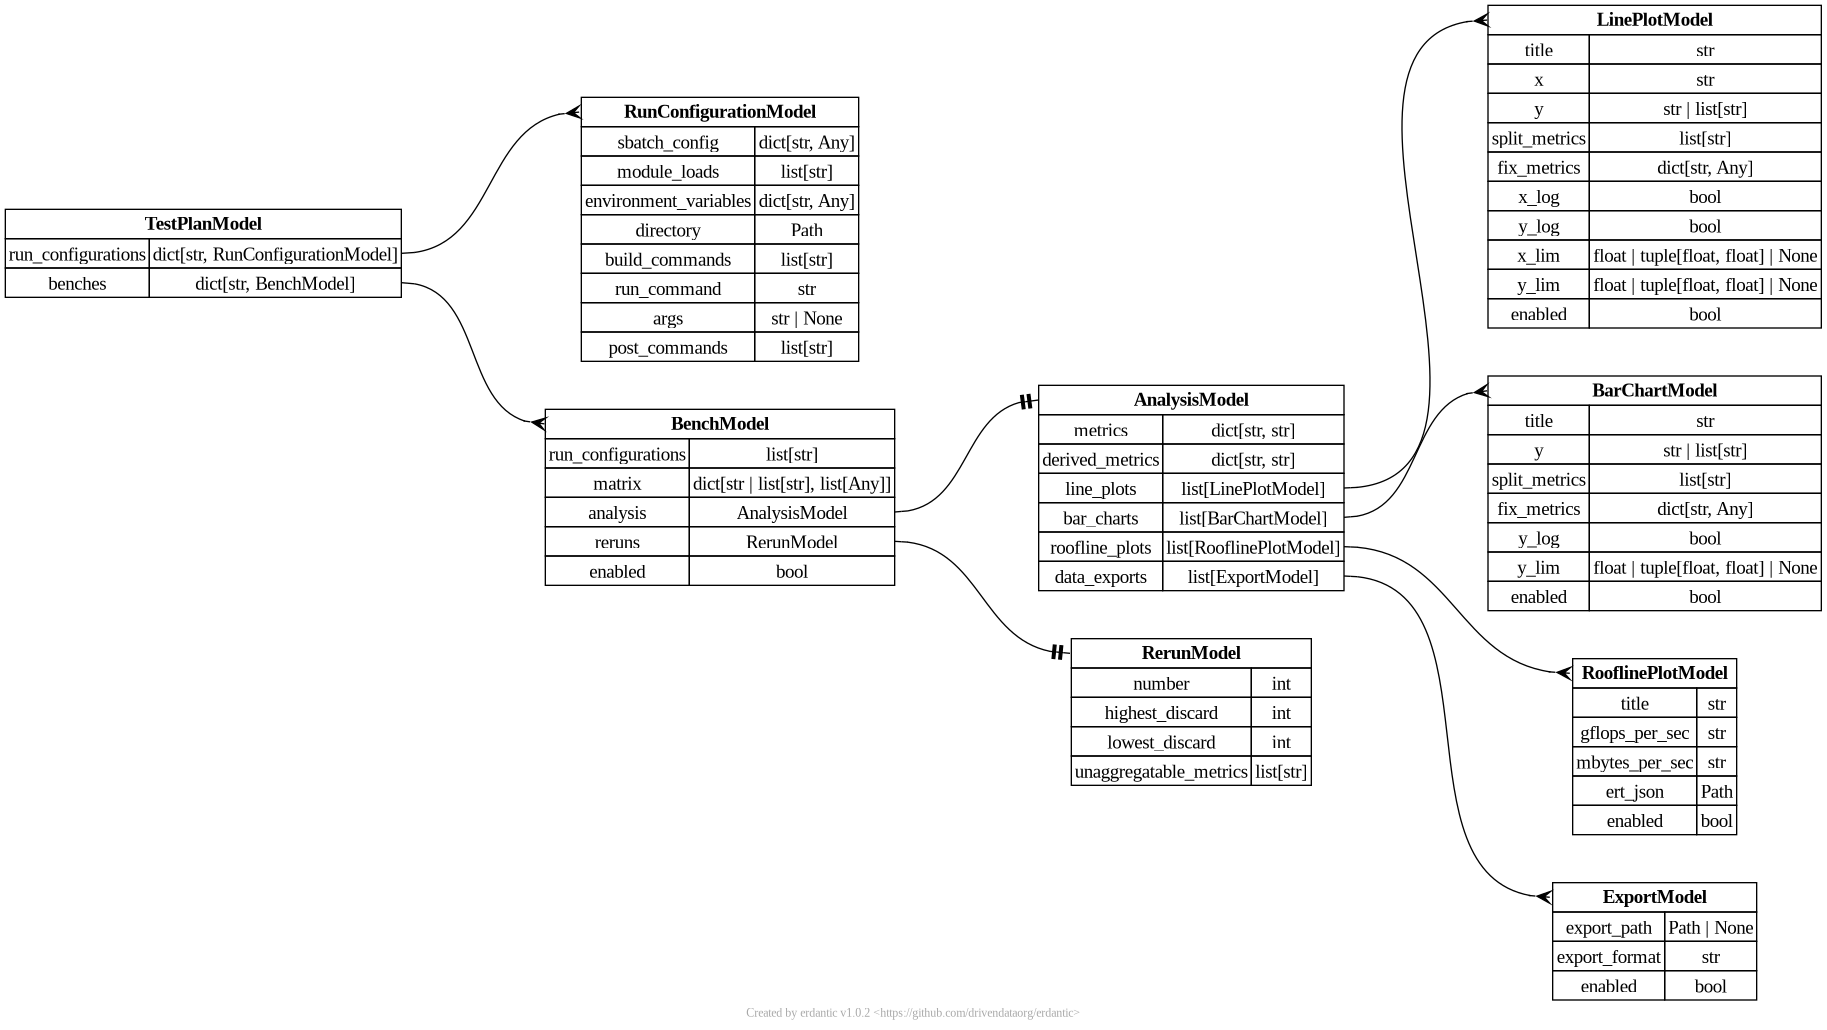
\includegraphics[width=\textwidth]{images/4_tooling/implementation/yaml_model.png}
    \caption{An entity-relationship diagram showing the Pydantic model representing the YAML schema, generated using the \texttt{erdantic} tool.}
    \label{fig:hpc-multibench-yaml-model}
\end{figure}

\subsection{Data flow}
\label{ssec:hpc-multibench-data-flow}

Having parsed the configuration data, the majority of the application logic implements the data processing pipeline to create and run the instantations, then extract metrics from and aggregate the results. These data flows are depicted in Figure \ref{fig:hpc-multibench-data-flow}, and are described in more detail in the docstring-generated documentation for the \textit{test bench} class \url{https://edmundgoodman.co.uk/hpc-multibench/reference/test_bench.html}.

\begin{figure}[H]
    \centering
    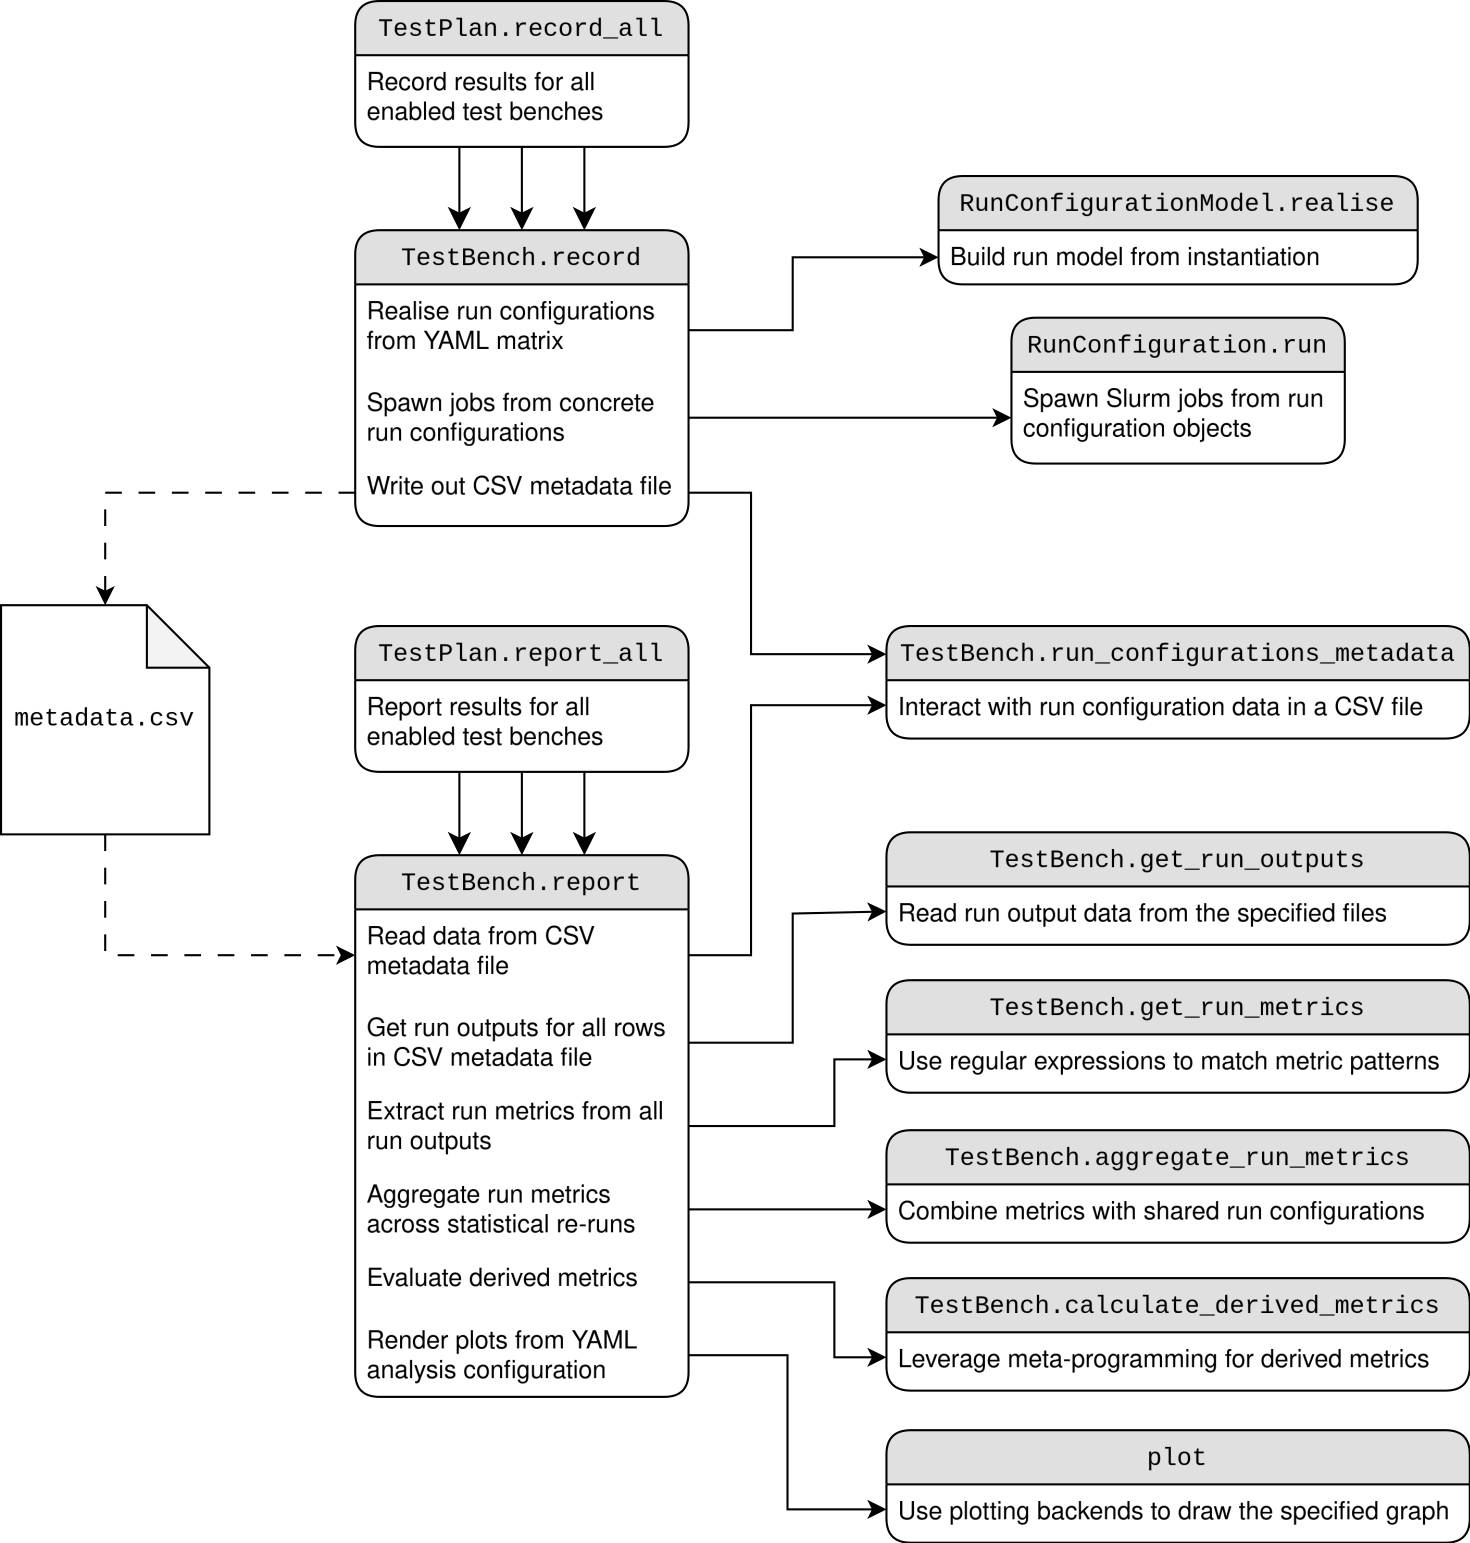
\includegraphics[width=0.75\textwidth]{images/4_tooling/implementation/hpc_multibench_data_flow.png}
    \caption{A diagram showing the data flow through the HPC MultiBench tool.}
    \label{fig:hpc-multibench-data-flow}
\end{figure}

In this diagram, we can see that the record and report phases operate completely independently of each of, sharing information through the \texttt{metadata.csv} file. This allows experiments to be run asynchronously, avoiding problems caused by dropped \texttt{ssh} connections without requiring tools such as \texttt{tmux}.

\subsection{User interface}
\label{ssec:hpc-multibench-ui}

A key design goal of the project was providing an interactive user interface, which can run on remote machines without requiring setup such as configuring X-forwarding. This was motivated by the fact most High-Performance Computing resources are accessed over an SSH connection, which may be proxied through other servers. To mitigate this, X-forwarded graphical applications can be flaky or have very high latency. As a result of this, the tool was designed to have a simple command line interface, including a mode to render results interactively in the terminal without requiring X-forwarding.

The HPC MultiBench command-line user interface is designed to be familiar to users of existing tools, such as the performance profiler \texttt{perf}. Much like \texttt{perf}, it provides two verb subcommands, \texttt{record} and \texttt{report}. The \texttt{record} command asynchronously dispatches experimental runs via Slurm, and the \texttt{report} command aggregates and presents an analysis of the results of these runs.

In addition to these, the \texttt{interactive} subcommand uses the Textual \cite{TextualizeTextual2024} library to render an interactive user interface for dispatching and analysing runs entirely in the terminal. Figure \ref{fig:hpc-multibench-line-plotext-2} shows a screenshot of the interactive mode user interface with graph plotting capabilities, and more can screenshots be found in the documentation website gallery page \url{https://edmundgoodman.co.uk/hpc-multibench/gallery.html}.

\begin{figure}[H]
    \centering
    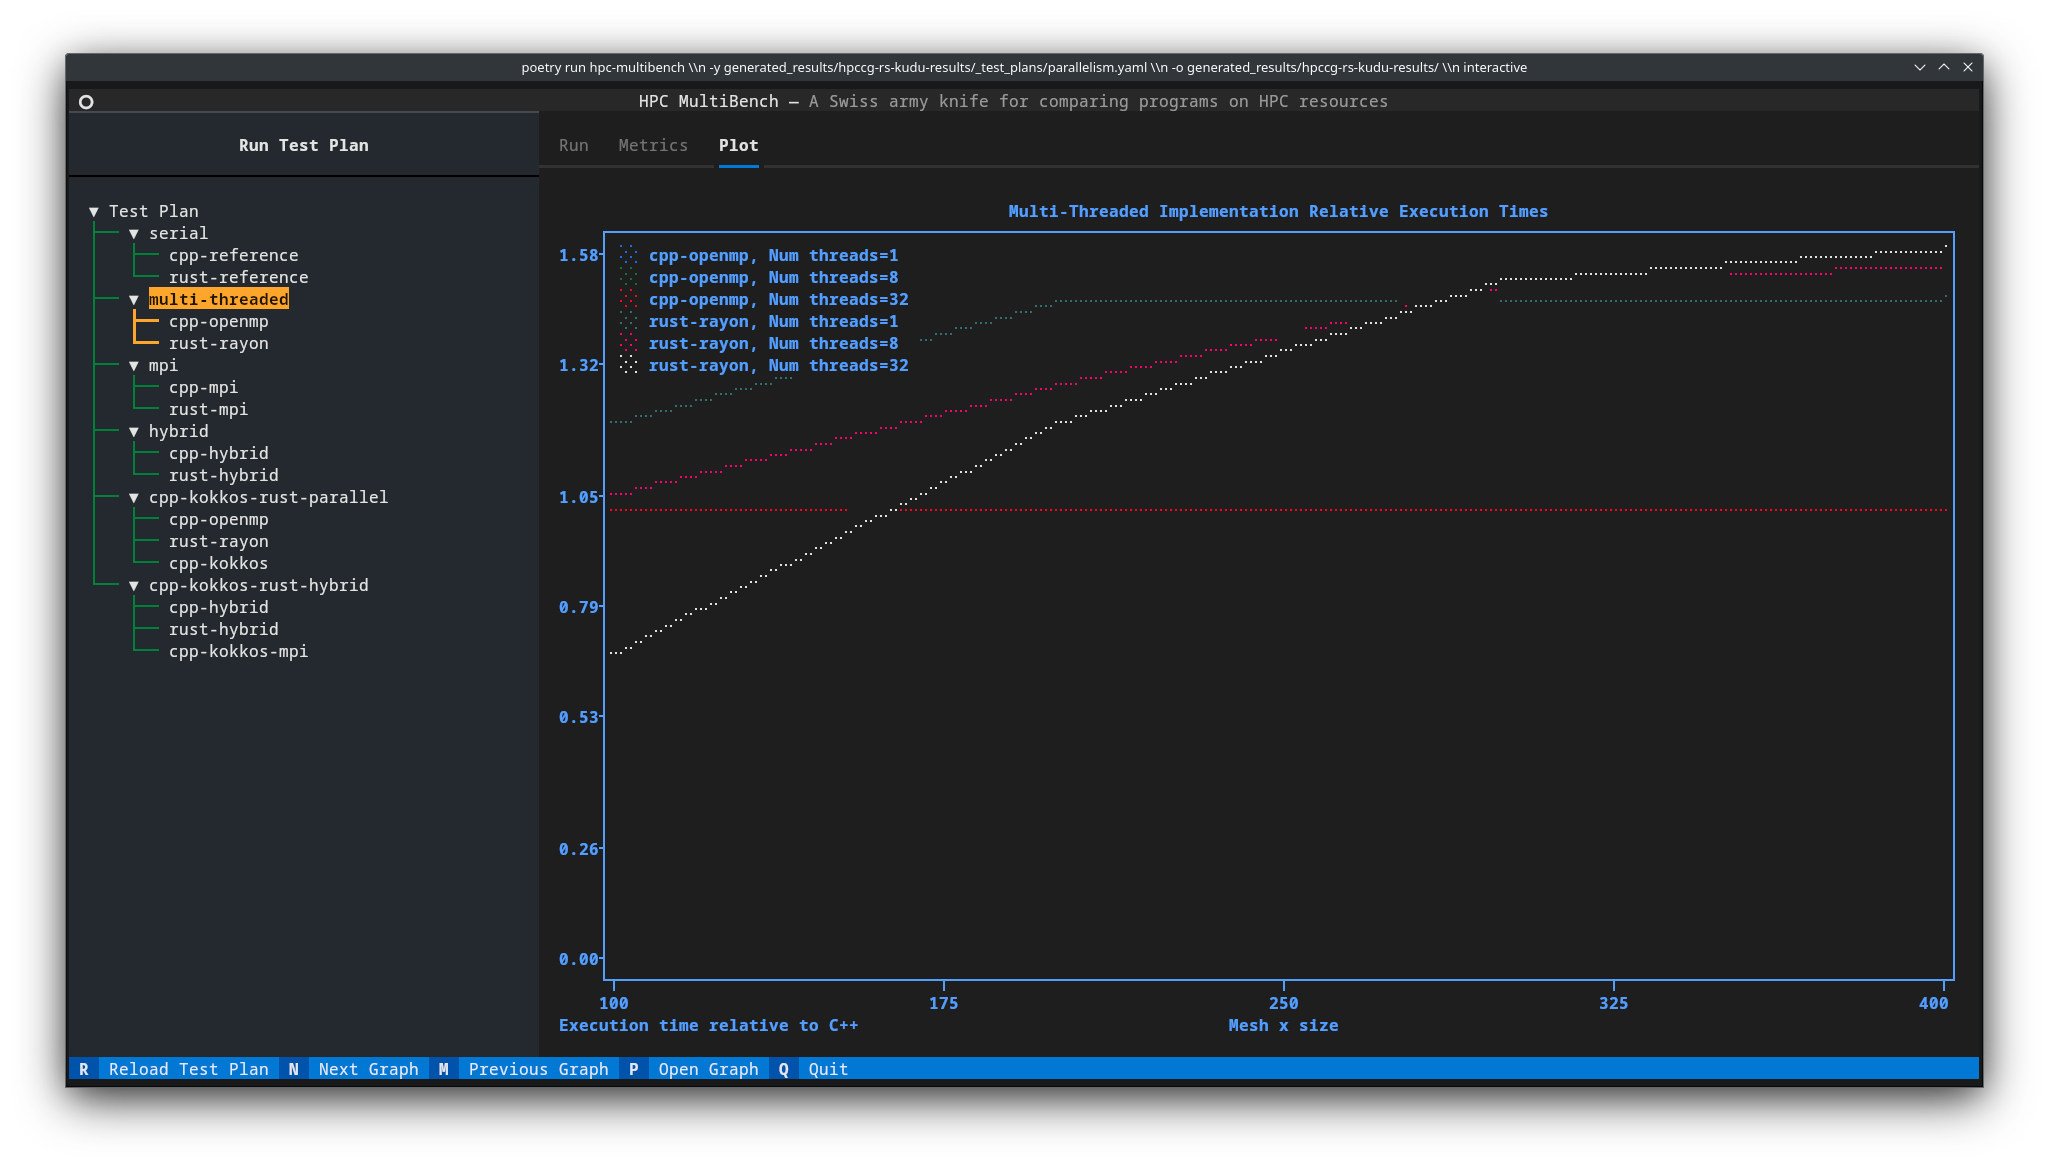
\includegraphics[width=\textwidth]{images/4_tooling/interactive_screenshots/hpc-multibench-line-plotext-2.png}
    \caption{A screenshot of the interactive mode user interface plotting a line graph, rendered entirely in the Terminal.}
    \label{fig:hpc-multibench-line-plotext-2}
\end{figure}

\subsection{Developer tooling and documentation}
\label{ssec:hpc-multibench-developer-tooling-documentation}

For any software development project of non-trivial size, it is critical to leverage industry best practices to maximise productivity. Using the \texttt{scc} \cite{boyterBoyterScc2024} tool on the \texttt{src/} directory, HPC MultiBench was measured as 1572 lines of Python excluding blank space and code comments. Applying the COCOMO developer productivity model used by \texttt{scc} and as discussed in \Cref{ch:background}, this is estimated to take 4.18 months to develop, and cost \$43,438 in an average industry setting. Due to the author's experience building such tools, and current occupation as a student, significantly less time and no cost was required to undertake this development.

To ensure that the development was completed on time, best practices such as \texttt{git} for version control were leveraged. In addition to this, more esoteric tooling such as pre-commit hooks to run linters and type checkers, along with continuous integration infrastructure, allowed software bugs to be caught early.

For a software tool to be adopted, users must be able to install it, run it, and apply it to their use cases. As a result of this, documentation is required to explain to users how to perform these steps. As part of its continuous integration infrastructure, HPC MultiBench generates a documentation website generated from markdown and docstrings in the python source code using \texttt{MkDocs-Material} framework \cite{donathSquidfunkMkdocsmaterial2024}, which is then deployed as a static site hosted on GitHub pages. This documentation site can be found at \url{https://edmundgoodman.co.uk/hpc-multibench/}, with a screenshot of the splash page shown in Figure \ref{fig:documentation_splash}.

\begin{figure}[H]
    \centering
    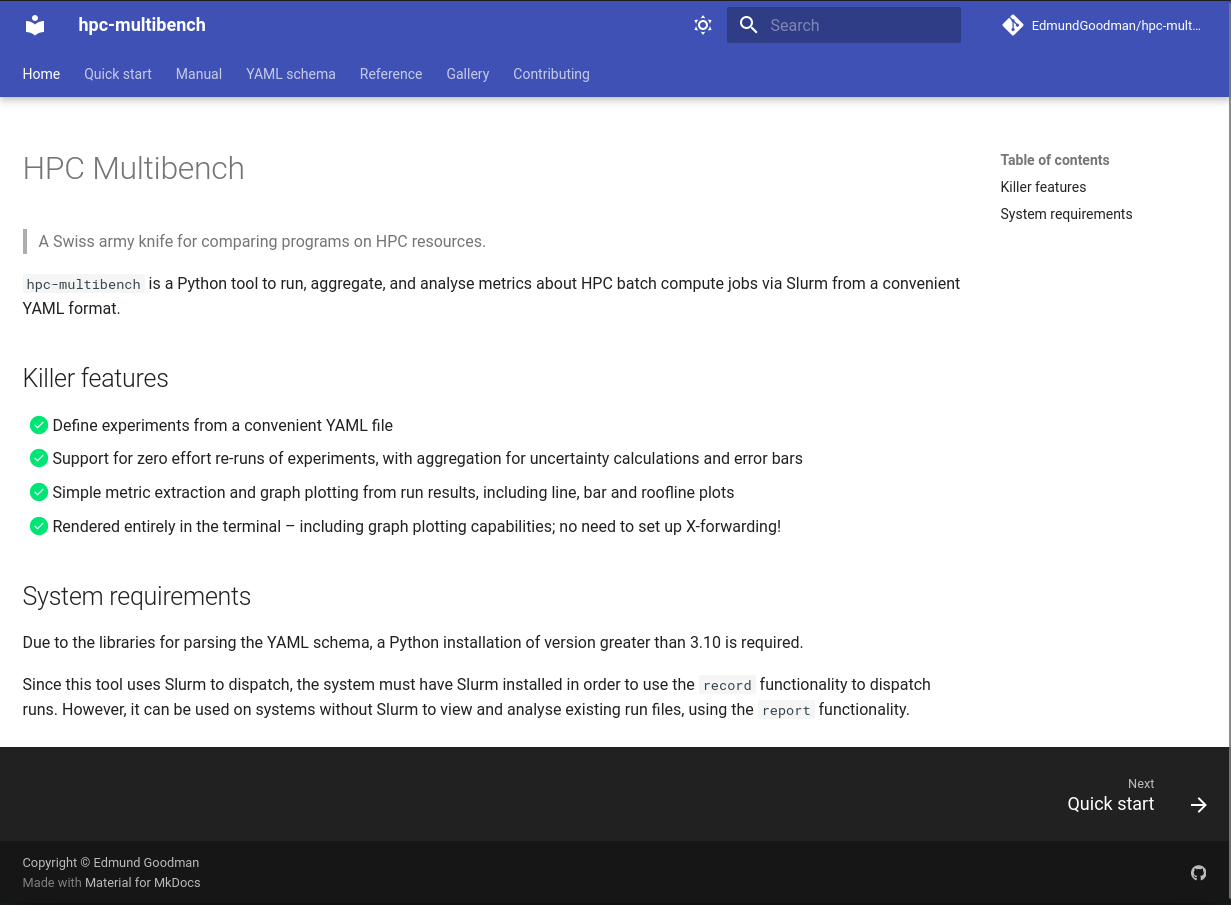
\includegraphics[width=\textwidth]{images/4_tooling/implementation/documentation_splash.png}
    \caption{A screenshot of the documentation website splash page for the HPC MultiBench tool, hosted at \url{https://edmundgoodman.co.uk/hpc-multibench/}.}
    \label{fig:documentation_splash}
\end{figure}

% TODO: Could add screenshot of the auto-generated docs from docstrings

% TODO: Is this needed?
In addition to this, as part of the the open source contributions made by this project, discussed in \ref{sec:open-source-work}, this tool will be made public on GitHub once the assessment phase of the module has finished. In addition to this, it will be released to PyPI -- allowing it to be installed with a single command using Python's package manage, \texttt{pip}.


\section{Example use case}
\label{sec:hpc-multibench-example-use-case}

As discussed in section \ref{sec:hpc-multibench-motivation}, a key motivation for this tool is streamlining the tedious process of manually running, aggregating, and analysing the results of many program runs to create a statistically confident characterisation of the performance of programs. Since this process is so time-consuming, due to both the process of conducting many runs, and re-writing scripts to aggregate and present the data, it is often not viable to spend time running replication studies of existing work, despite the benefits many benefits this work provides. Beyond the clear use case for this tool of running and analysing original results, which is showcased in full in \Cref{ch:performance}, this tool also makes it possible to very quickly conduct replication studies of existing work in the field.

In his paper ``Shall we Really do it Again? The Powerful Concept of Replication is Neglected in the Social Sciences'', Schmidt introduces replication as ``one of the central issues in any empirical science'', and goes on to define replication studies as ``'' \cite{schmidtShallWeReally2009}. In recent years, the absence of reproducible results in publications has been branded the ``replication crisis'', with Ioannidis publishing a paper title ``Why Most Published Research Findings Are False'' on the basis of a very high rate of non-reproducibility of experimental data \cite{ioannidisWhyMostPublished2005}. Since High-Performance computing relies on many empirical measurements to draw conclusions about characteristics of hardware and software, tooling to facilitate reproducibility is clearly desirable.

\subsection{Replication study of ``Emerging technologies: Rust in HPC''}
\label{ssec:hpc-multibench-replication-study}

This section shows the workflow of running a replication study on Moran and Bull's paper ``Emerging technologies: Rust in HPC'' \cite{moranEmergingTechnologiesRust2023}. This paper was selected as the source code is available as a GitHub repo \cite{Lmoran94Eurocc_cfdCFD}, and the paper draws a different conclusion to other existing work such as Constanza et al. \cite{costanzoPerformanceVsProgramming2021}, so replication would either provide confidence in their results, or elucidate any possible reasons for this difference.

As a result of the focussed design goals of the HPC MultiBench tool, the workflow for the replication study facilitated by the HPC MultiBench tool is exceedingly simple, consisting of six short steps -- each of which requires only one terminal command:

\begin{enumerate}
    \item Clone the HPC MultiBench tool repository
    \item Install the HPC MultiBench tool using \texttt{poetry}
    \item Add the GitHub repository containing the source code as a submodule
    \item Write a YAML file defining the run configurations and analysis presented in the paper
    \item Use the \texttt{record} command of the HPC MultiBench tool to run the jobs defined by the YAML file
    \item Use the \texttt{report} command of the HPC MultiBench tool to run analyse the results defined by the YAML file
\end{enumerate}

Listing \ref{listing:replication-study-workflow} shows the six terminal commands required to perform these six steps.

% TODO: Consider framing all listings with [linenos,breaklines,frame=single]
% TODO: Submoduling strategy has changed, update to reflect this
\begin{code}
    %TC:ignore
    \begin{minted}{bash}
        git clone https://github.com/EdmundGoodman/hpc-multibench
        poetry install --without docs,test,dev
        git submodule add https://github.com/lmoran94/eurocc_cfd generated_results/
        vim generated_results/replication_study.yaml  # The YAML file representing the paper is written here
        poetry run hpc_multibench \
            -y generated_results/replication_study.yaml record
        poetry run hpc_multibench \
            -y generated_results/replication_study.yaml report
    \end{minted}
    %TC:endignore
    \caption{A listing of the six bash commands required to run a full replication study of Moran and Bull's paper ``Emerging technologies: Rust in HPC'' \cite{moranEmergingTechnologiesRust2023}.}
    \label{listing:replication-study-workflow}
\end{code}

The necessary complexity to represent the unique aspects of the results being replicated is encoded in the YAML file, which is shown in Listing \ref{listing:replication-study-workflow} as being written in \texttt{vim}. This is the most involved part of the process, but the abstractions in the design of the YAML schema are designed to make it as simple as possible, whilst still being able to represent most common analyses done by papers.

A full listing of the YAML file for the replication study is provided in Appendix \ref{sec:tooling-replication-yaml}. It is only 190 lines long, much of which can be templated from examples in the tool documentation. This is significantly shorter in line length than the code that would be required to script running all the configurations of the programs, aggregating the results, and plotting graphs for them -- and avoids much of the time spent debugging that would be required for writing such custom scripts. Examples of the original and replicated figures from the paper are shown pairwise in figures \ref{fig:replication_mine_1}, \ref{fig:replication_original_1}, \ref{fig:replication_mine_2}, \ref{fig:replication_original_2}, \ref{fig:replication_mine_4}, and \ref{fig:replication_original_4}.

\newpage
\begin{figure}[H]
    \centering
    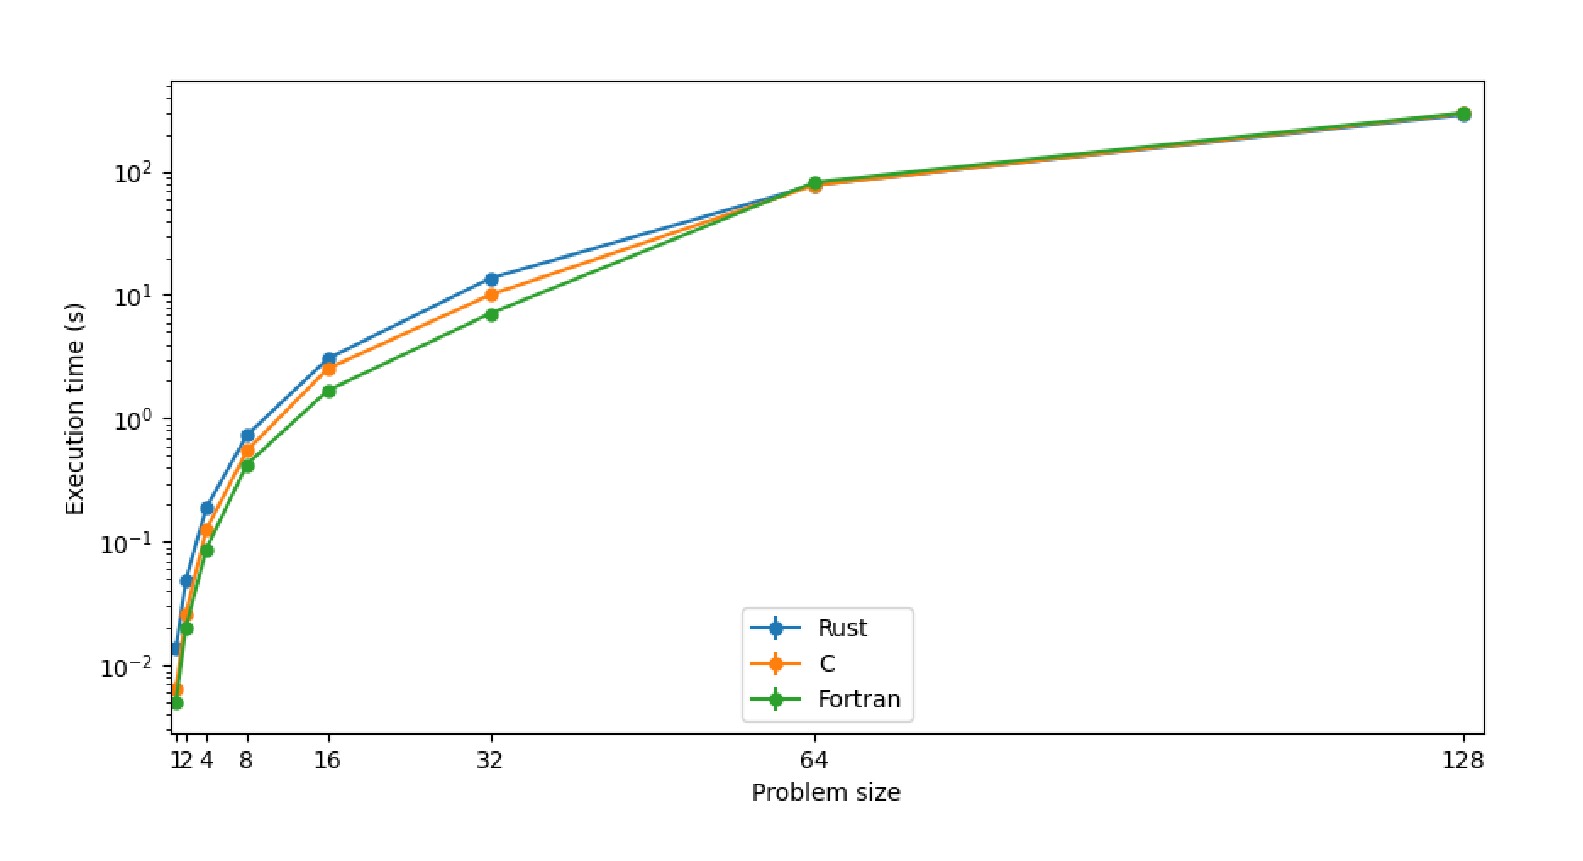
\includegraphics[width=\textwidth]{images/4_tooling/replication_study/replication_original_1.png}
    \caption{A plot comparing total time taken for a serial codebase, from Moran and Bull's paper \cite{moranEmergingTechnologiesRust2023}.}
    \label{fig:replication_original_1}
\end{figure}
\begin{figure}[H]
    \centering
    % This file was created with tikzplotlib v0.10.1.
\begin{tikzpicture}

\definecolor{darkorange25512714}{RGB}{255,127,14}
\definecolor{darkslategray38}{RGB}{38,38,38}
\definecolor{forestgreen4416044}{RGB}{44,160,44}
\definecolor{lightgray204}{RGB}{204,204,204}
\definecolor{steelblue31119180}{RGB}{31,119,180}

\begin{axis}[
axis line style={lightgray204},
height=0.45\textheight,
legend cell align={left},
legend style={
  fill opacity=0.8,
  draw opacity=1,
  text opacity=1,
  at={(0.03,0.97)},
  anchor=north west,
  draw=none
},
log basis y={10},
tick align=outside,
tick pos=left,
title={Serial Implementation Comparison},
width=\textwidth,
x grid style={lightgray204},
xlabel=\textcolor{darkslategray38}{Problem size},
xmajorgrids,
xmin=-5.35, xmax=134.35,
xtick style={color=darkslategray38},
y grid style={lightgray204},
ylabel=\textcolor{darkslategray38}{Total time (s)},
ymajorgrids,
ymin=0.00276962091188793, ymax=479.472792233479,
ymode=log,
ytick style={color=darkslategray38},
ytick={0.0001,0.001,0.01,0.1,1,10,100,1000,10000},
yticklabels={
  $\mathdefault{10^{-4}}$,
  $\mathdefault{10^{-3}}$,
  $\mathdefault{10^{-2}}$,
  $\mathdefault{10^{-1}}$,
  $\mathdefault{10^{0}}$,
  $\mathdefault{10^{1}}$,
  $\mathdefault{10^{2}}$,
  $\mathdefault{10^{3}}$,
  $\mathdefault{10^{4}}$
}
]
\path [draw=black, semithick]
(axis cs:1,0.00699695619045528)
--(axis cs:1,0.00714889980954473);

\path [draw=black, semithick]
(axis cs:2,0.0248998488334846)
--(axis cs:2,0.0253484291665154);

\path [draw=black, semithick]
(axis cs:4,0.0995044073930531)
--(axis cs:4,0.104492018206947);

\path [draw=black, semithick]
(axis cs:8,0.453278231698825)
--(axis cs:8,0.462615895501175);

\path [draw=black, semithick]
(axis cs:16,1.87885480947366)
--(axis cs:16,1.91419551012634);

\path [draw=black, semithick]
(axis cs:32,7.67157472162308)
--(axis cs:32,7.82571970997692);

\path [draw=black, semithick]
(axis cs:64,60.6741855487599)
--(axis cs:64,63.8700804404401);

\path [draw=black, semithick]
(axis cs:128,242.655782851411)
--(axis cs:128,251.361585132589);

\path [draw=black, semithick]
(axis cs:1,0.00550512106523007)
--(axis cs:1,0.00581404293476993);

\path [draw=black, semithick]
(axis cs:2,0.0218687301379282)
--(axis cs:2,0.0221087098620718);

\path [draw=black, semithick]
(axis cs:4,0.102995548000624)
--(axis cs:4,0.117852131999376);

\path [draw=black, semithick]
(axis cs:8,0.453730961579502)
--(axis cs:8,0.471573038420498);

\path [draw=black, semithick]
(axis cs:16,1.91848746920254)
--(axis cs:16,1.96192453079745);

\path [draw=black, semithick]
(axis cs:32,7.80141277650708)
--(axis cs:32,7.90499122349292);

\path [draw=black, semithick]
(axis cs:64,61.7663163440984)
--(axis cs:64,64.4131636559016);

\path [draw=black, semithick]
(axis cs:128,246.217606721236)
--(axis cs:128,254.281593278764);

\path [draw=black, semithick]
(axis cs:1,0.00479211088514963)
--(axis cs:1,0.00485548911485037);

\path [draw=black, semithick]
(axis cs:2,0.0257170868079985)
--(axis cs:2,0.0259589131920015);

\path [draw=black, semithick]
(axis cs:4,0.0939223678966043)
--(axis cs:4,0.0998856321033957);

\path [draw=black, semithick]
(axis cs:8,0.445380601935724)
--(axis cs:8,0.449699398064276);

\path [draw=black, semithick]
(axis cs:16,1.81830026455212)
--(axis cs:16,1.85609973544788);

\path [draw=black, semithick]
(axis cs:32,6.98108506186961)
--(axis cs:32,7.16251493813039);

\path [draw=black, semithick]
(axis cs:64,66.4810246754828)
--(axis cs:64,70.3309753245172);

\path [draw=black, semithick]
(axis cs:128,262.486656031609)
--(axis cs:128,277.113343968391);

\addplot [semithick, steelblue31119180, mark=x, mark size=3, mark options={solid}]
table {%
1 0.00707292603328824
2 0.0251241382211447
4 0.101998224854469
8 0.457947015762329
16 1.89652526378632
32 7.74864625930786
64 62.2721366882324
128 247.00862121582
};
\addlegendentry{Rust}
\addplot [semithick, darkorange25512714, mark=x, mark size=3, mark options={solid}]
table {%
1 0.00565958069637418
2 0.0219887178391218
4 0.110423862934113
8 0.462652027606964
16 1.94020617008209
32 7.85320091247559
64 63.0897369384766
128 250.249588012695
};
\addlegendentry{C++}
\addplot [semithick, forestgreen4416044, mark=x, mark size=3, mark options={solid}]
table {%
1 0.0048237987793982
2 0.0258379988372326
4 0.0969040021300316
8 0.447539955377579
16 1.83720004558563
32 7.07180023193359
64 68.406005859375
128 269.800018310547
};
\addlegendentry{FORTRAN}
\end{axis}

\end{tikzpicture}

    \vspace*{-0.5cm}
    % 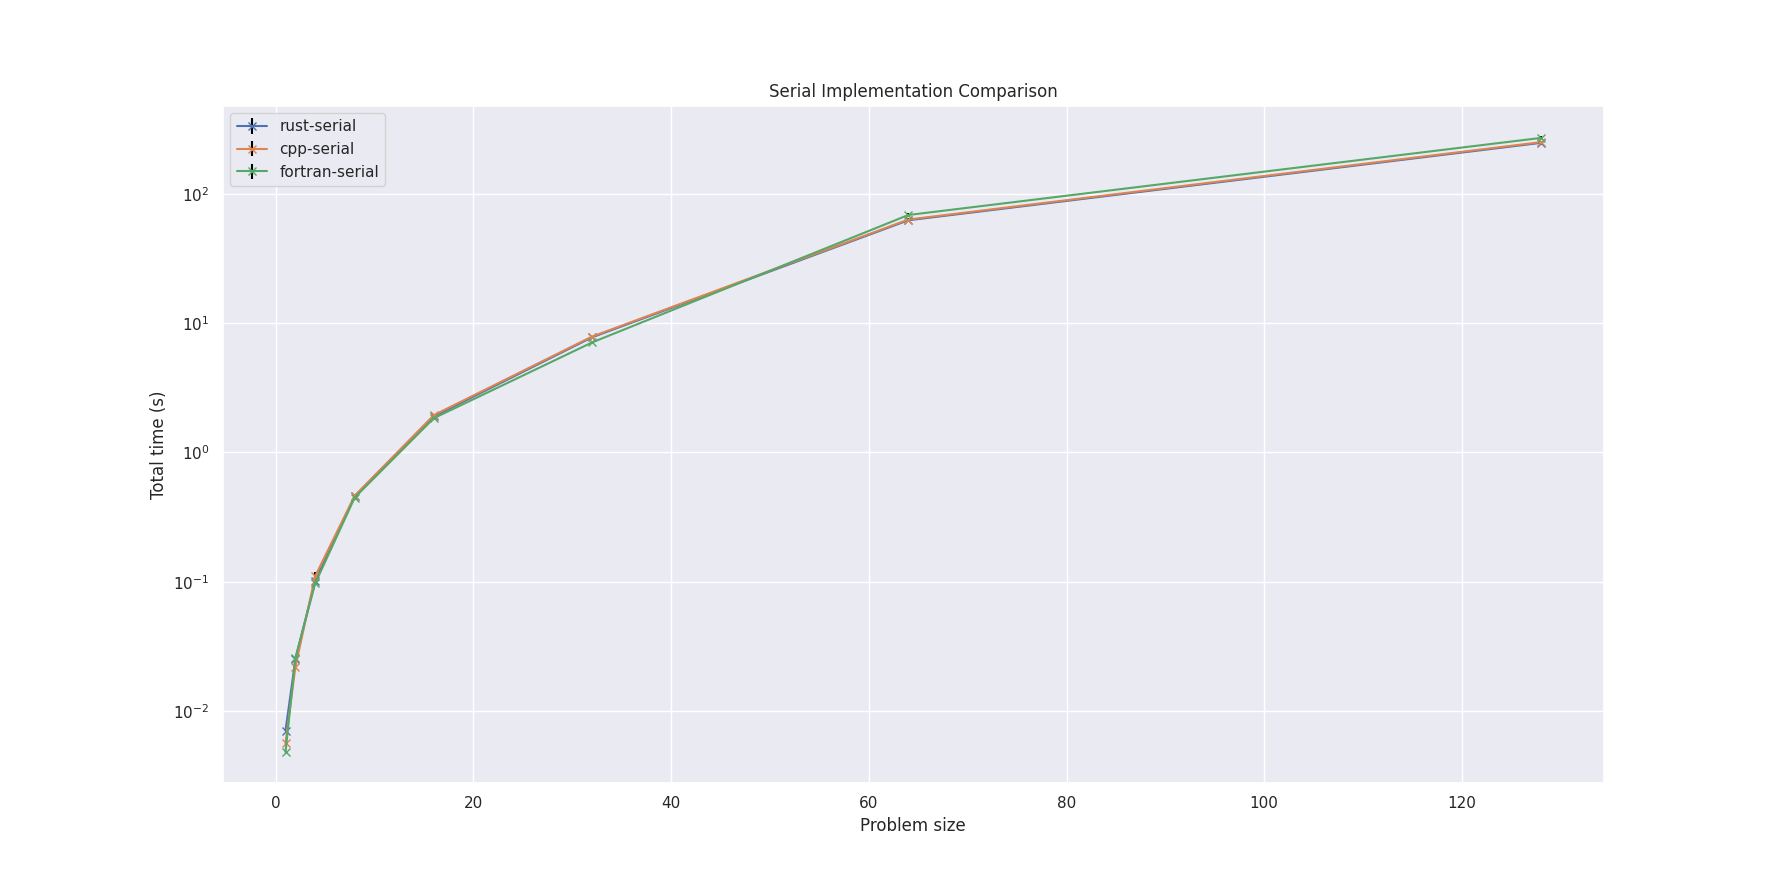
\includegraphics[width=\textwidth]{images/4_tooling/replication_study/replication_mine_1.png}
    \caption{A plot comparing total time taken for a serial codebase, replicated using HPC MultiBench.}
    \label{fig:replication_mine_1}
\end{figure}


\begin{figure}[H]
    \centering
    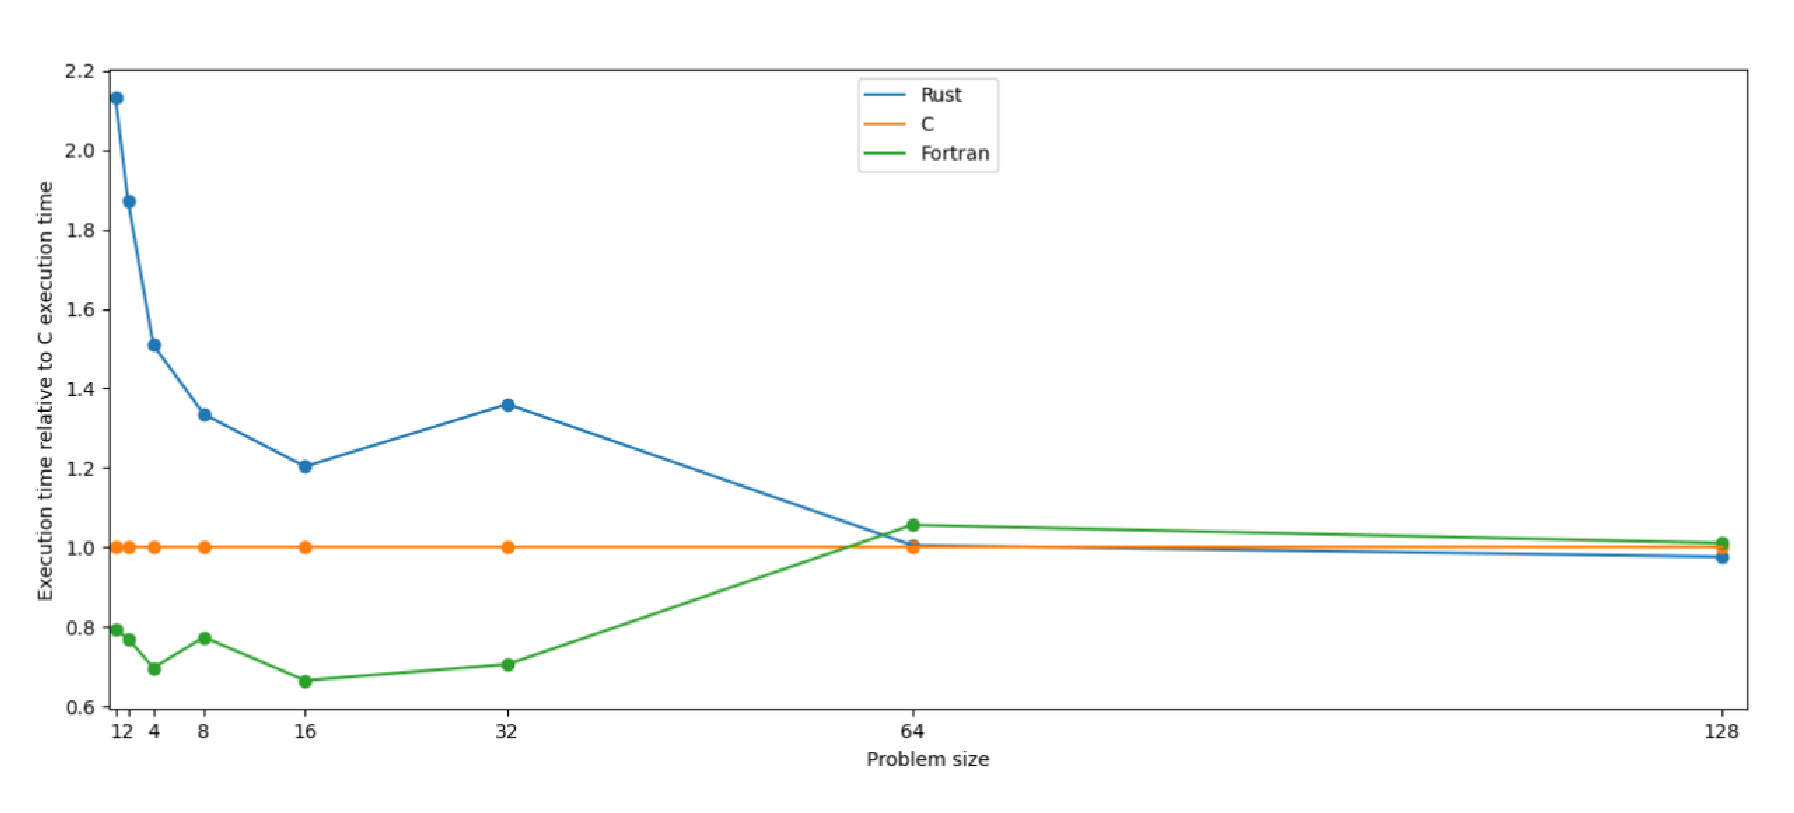
\includegraphics[width=\textwidth]{images/4_tooling/replication_study/replication_original_2.png}
    \caption{A plot comparing serial execution times relative to C++, from Moran and Bull's paper \cite{moranEmergingTechnologiesRust2023}.}
    \label{fig:replication_original_2}
\end{figure}
\begin{figure}[H]
    \centering
    % This file was created with tikzplotlib v0.10.1.
\begin{tikzpicture}

\definecolor{darkorange25512714}{RGB}{255,127,14}
\definecolor{darkslategray38}{RGB}{38,38,38}
\definecolor{forestgreen4416044}{RGB}{44,160,44}
\definecolor{lightgray204}{RGB}{204,204,204}
\definecolor{steelblue31119180}{RGB}{31,119,180}

\begin{axis}[
axis line style={lightgray204},
height=0.35\textheight,
legend cell align={left},
legend style={fill opacity=0.8, draw opacity=1, text opacity=1, draw=none},
tick align=outside,
tick pos=left,
title={Relative execution times to C++},
width=\textwidth,
x grid style={lightgray204},
xlabel=\textcolor{darkslategray38}{Problem size},
xmajorgrids,
xmin=-5.35, xmax=134.35,
xtick style={color=darkslategray38},
y grid style={lightgray204},
ylabel=\textcolor{darkslategray38}{Execution time relative to C++},
ymajorgrids,
ymin=0.6, ymax=2.2,
ytick style={color=darkslategray38}
]
\path [draw=black, semithick]
(axis cs:1,1.21306956345733)
--(axis cs:1,1.28637933655133);

\path [draw=black, semithick]
(axis cs:2,1.13063718355118)
--(axis cs:2,1.15454712913278);

\path [draw=black, semithick]
(axis cs:4,0.857582528428346)
--(axis cs:4,0.989812920741126);

\path [draw=black, semithick]
(axis cs:8,0.968240592274161)
--(axis cs:8,1.01142042118736);

\path [draw=black, semithick]
(axis cs:16,0.963247757033249)
--(axis cs:16,0.991723214945013);

\path [draw=black, semithick]
(axis cs:32,0.974911442893033)
--(axis cs:32,0.998461759317531);

\path [draw=black, semithick]
(axis cs:64,0.95432553212862)
--(axis cs:64,1.01975373249419);

\path [draw=black, semithick]
(axis cs:128,0.963482123549343)
--(axis cs:128,1.01061798611725);

\path [draw=black, semithick]
(axis cs:1,1)
--(axis cs:1,1);

\path [draw=black, semithick]
(axis cs:2,1)
--(axis cs:2,1);

\path [draw=black, semithick]
(axis cs:4,1)
--(axis cs:4,1);

\path [draw=black, semithick]
(axis cs:8,1)
--(axis cs:8,1);

\path [draw=black, semithick]
(axis cs:16,1)
--(axis cs:16,1);

\path [draw=black, semithick]
(axis cs:32,1)
--(axis cs:32,1);

\path [draw=black, semithick]
(axis cs:64,1)
--(axis cs:64,1);

\path [draw=black, semithick]
(axis cs:128,1)
--(axis cs:128,1);

\path [draw=black, semithick]
(axis cs:1,0.828389558156663)
--(axis cs:1,0.876221553248934);

\path [draw=black, semithick]
(axis cs:2,1.16659640860399)
--(axis cs:2,1.18369956132969);

\path [draw=black, semithick]
(axis cs:4,0.812582689590874)
--(axis cs:4,0.942473738461775);

\path [draw=black, semithick]
(axis cs:8,0.94811121590957)
--(axis cs:8,0.986561064767915);

\path [draw=black, semithick]
(axis cs:16,0.932688005064488)
--(axis cs:16,0.961335728473359);

\path [draw=black, semithick]
(axis cs:32,0.88740876207216)
--(axis cs:32,0.913385818480991);

\path [draw=black, semithick]
(axis cs:64,1.04620045840618)
--(axis cs:64,1.12245437961835);

\path [draw=black, semithick]
(axis cs:128,1.04397360983739)
--(axis cs:128,1.11219539596243);

\addplot [semithick, steelblue31119180, mark=x, mark size=3, mark options={solid}]
table {%
1 1.24972450733185
2 1.14259219169617
4 0.923697710037231
8 0.989830493927002
16 0.977485418319702
32 0.986686587333679
64 0.987039566040039
128 0.98705005645752
};
\addlegendentry{Rust}
\addplot [semithick, darkorange25512714, mark=x, mark size=3, mark options={solid}]
table {%
1 1
2 1
4 1
8 1
16 1
32 1
64 1
128 1
};
\addlegendentry{C++}
\addplot [semithick, forestgreen4416044, mark=x, mark size=3, mark options={solid}]
table {%
1 0.85230553150177
2 1.17514801025391
4 0.877528190612793
8 0.967336177825928
16 0.947011947631836
32 0.900397300720215
64 1.08432745933533
128 1.07808446884155
};
\addlegendentry{FORTRAN}
\end{axis}

\end{tikzpicture}

    \vspace*{-0.5cm}
    % 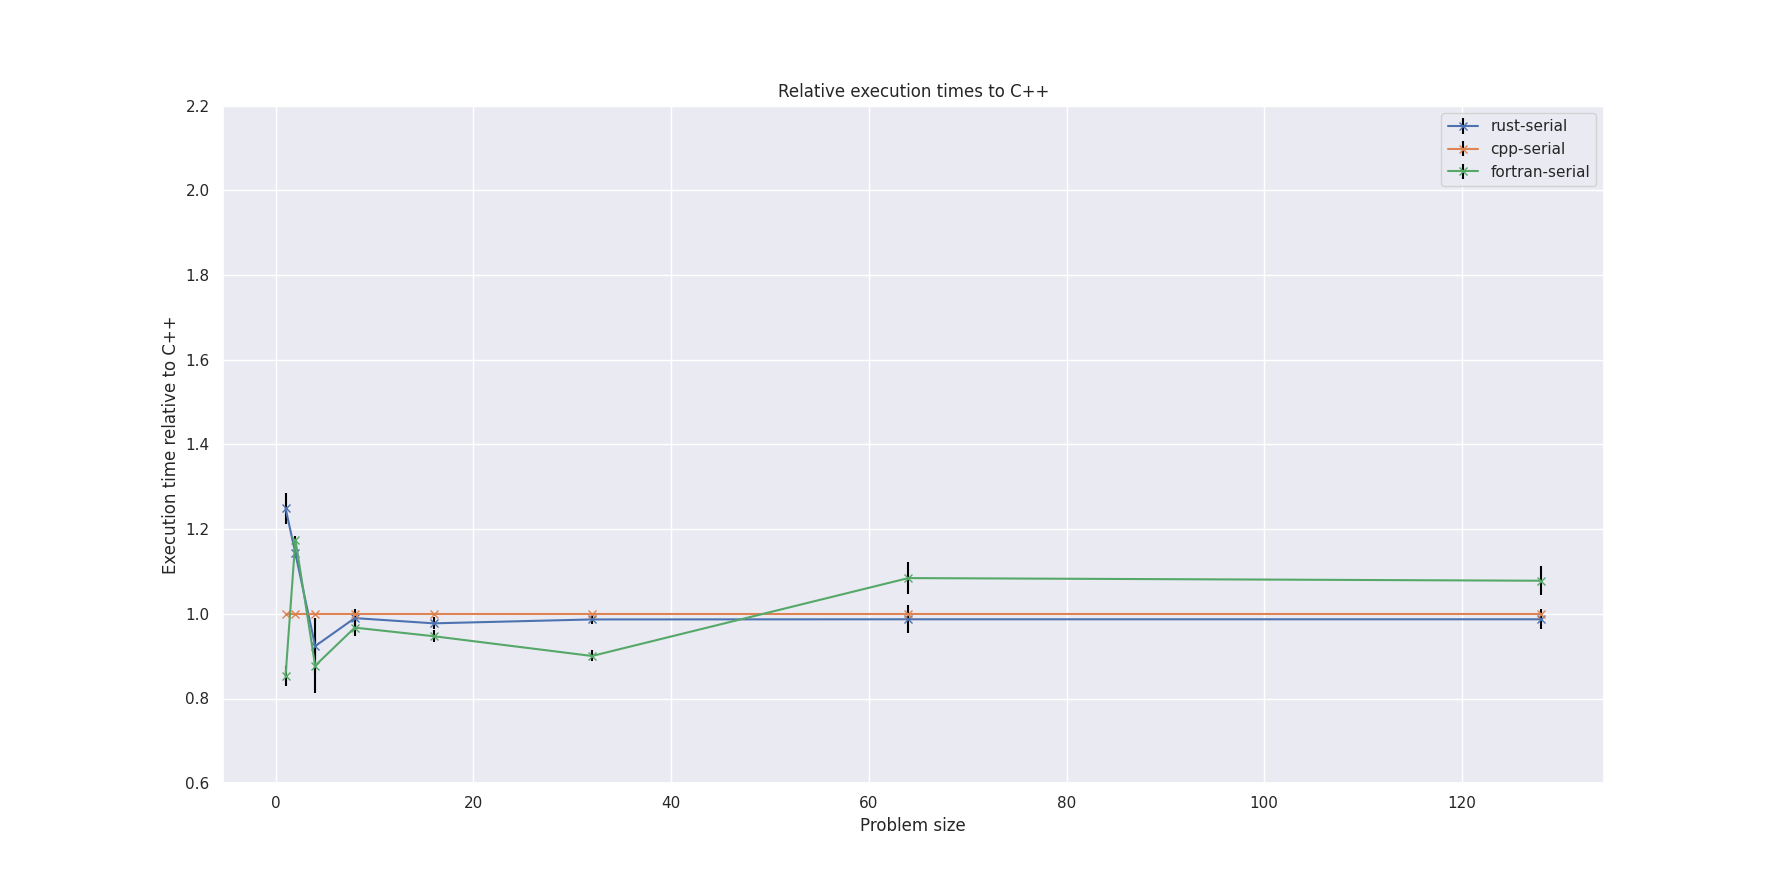
\includegraphics[width=\textwidth]{images/4_tooling/replication_study/replication_mine_2.png}
    \caption{A plot comparing serial execution times relative to C++, replicated using HPC MultiBench.}
    \label{fig:replication_mine_2}
\end{figure}


\begin{figure}[H]
    \centering
    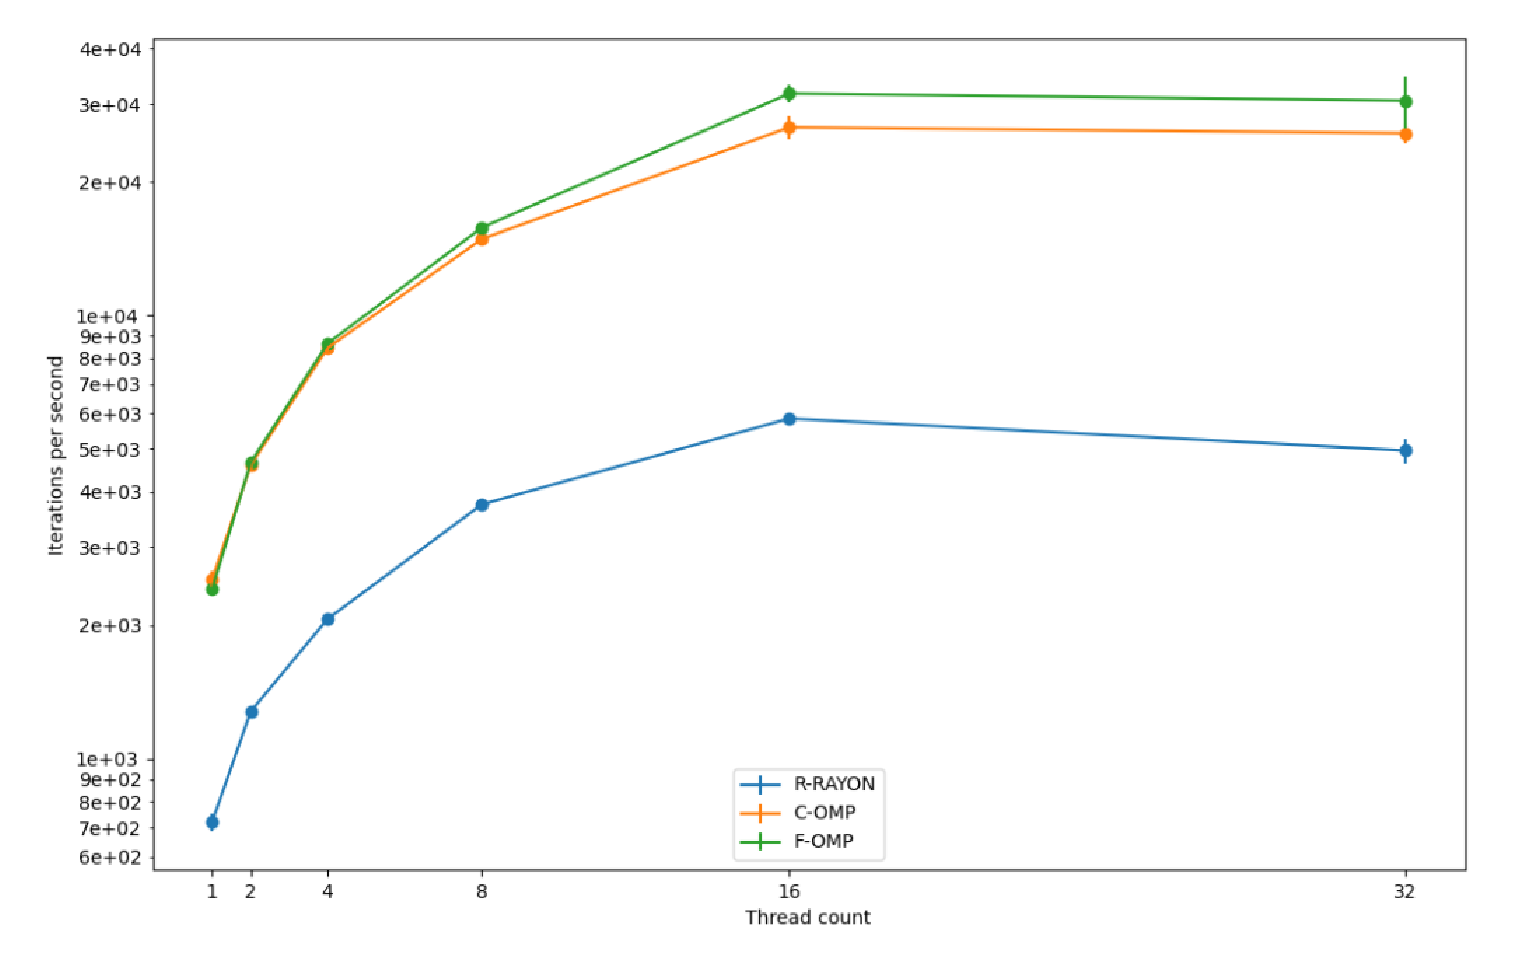
\includegraphics[width=0.9\textwidth]{images/4_tooling/replication_study/replication_original_4.png}
    \caption{A plot showing rate of iterations scaling with the number of threads used, from Moran and Bull's paper \cite{moranEmergingTechnologiesRust2023}.}
    \label{fig:replication_original_4}
\end{figure}
\begin{figure}[H]
    \centering
    % This file was created with tikzplotlib v0.10.1.
\begin{tikzpicture}

\definecolor{darkorange25512714}{RGB}{255,127,14}
\definecolor{darkslategray38}{RGB}{38,38,38}
\definecolor{forestgreen4416044}{RGB}{44,160,44}
\definecolor{lightgray204}{RGB}{204,204,204}
\definecolor{steelblue31119180}{RGB}{31,119,180}

\begin{axis}[
axis line style={lightgray204},
height=0.35\textheight,
legend cell align={left},
legend style={
  fill opacity=0.8,
  draw opacity=1,
  text opacity=1,
  at={(0.97,0.03)},
  anchor=south east,
  draw=none
},
log basis y={10},
tick align=outside,
tick pos=left,
title={Iterations per second scaling with number of threads},
width=\textwidth,
x grid style={lightgray204},
xlabel=\textcolor{darkslategray38}{Thread count},
xmajorgrids,
xmin=-0.55, xmax=33.55,
xtick style={color=darkslategray38},
y grid style={lightgray204},
ylabel=\textcolor{darkslategray38}{Iterations per second},
ymajorgrids,
ymin=638.374132908277, ymax=27835.1456268058,
ymode=log,
ytick style={color=darkslategray38},
ytick={10,100,1000,10000,100000,1000000},
]
\path [draw=black, semithick]
(axis cs:1,757.877190131122)
--(axis cs:1,794.084221095316);

\path [draw=black, semithick]
(axis cs:2,1423.56762576161)
--(axis cs:2,1511.08340227299);

\path [draw=black, semithick]
(axis cs:4,2355.93121259758)
--(axis cs:4,2589.11008501284);

\path [draw=black, semithick]
(axis cs:8,3565.05146949343)
--(axis cs:8,3939.65093237861);

\path [draw=black, semithick]
(axis cs:16,3952.45920535198)
--(axis cs:16,4981.46042327058);

\path [draw=black, semithick]
(axis cs:32,3327.90004961904)
--(axis cs:32,4139.69859693642);

\path [draw=black, semithick]
(axis cs:1,2530.56787978821)
--(axis cs:1,2677.34231084213);

\path [draw=black, semithick]
(axis cs:2,4914.48241413384)
--(axis cs:2,5145.09037592891);

\path [draw=black, semithick]
(axis cs:4,8861.78756547661)
--(axis cs:4,9326.74383793228);

\path [draw=black, semithick]
(axis cs:8,15022.8819660373)
--(axis cs:8,15766.2622743299);

\path [draw=black, semithick]
(axis cs:16,16263.9883227418)
--(axis cs:16,16809.0382428361);

\path [draw=black, semithick]
(axis cs:32,20168.654246303)
--(axis cs:32,23446.0638019907);

\path [draw=black, semithick]
(axis cs:1,2554.73460354544)
--(axis cs:1,2659.30158186569);

\path [draw=black, semithick]
(axis cs:2,4920.73448236704)
--(axis cs:2,5120.43430968035);

\path [draw=black, semithick]
(axis cs:4,8807.91344932035)
--(axis cs:4,9571.06100390516);

\path [draw=black, semithick]
(axis cs:8,14914.957152596)
--(axis cs:8,15680.1170404589);

\path [draw=black, semithick]
(axis cs:16,14743.3419260503)
--(axis cs:16,21347.3178112096);

\path [draw=black, semithick]
(axis cs:32,17496.9748323564)
--(axis cs:32,21908.7862899197);

\addplot [semithick, steelblue31119180, mark=x, mark size=3, mark options={solid}]
table {%
1 775.980590820312
2 1467.32580566406
4 2472.52026367188
8 3752.3525390625
16 4466.95947265625
32 3733.79907226562
};
\addlegendentry{Rust, problem size=16}
\addplot [semithick, darkorange25512714, mark=x, mark size=3, mark options={solid}]
table {%
1 2603.95483398438
2 5029.7861328125
4 9094.265625
8 15394.5654296875
16 16536.509765625
32 21807.35546875
};
\addlegendentry{C++, problem size=16}
\addplot [semithick, forestgreen4416044, mark=x, mark size=3, mark options={solid}]
table {%
1 2607.0185546875
2 5020.5830078125
4 9189.4853515625
8 15297.5302734375
16 18045.330078125
32 19702.888671875
};
\addlegendentry{FORTRAN, problem size=16}
\end{axis}

\end{tikzpicture}

    \vspace*{-0.5cm}
    % 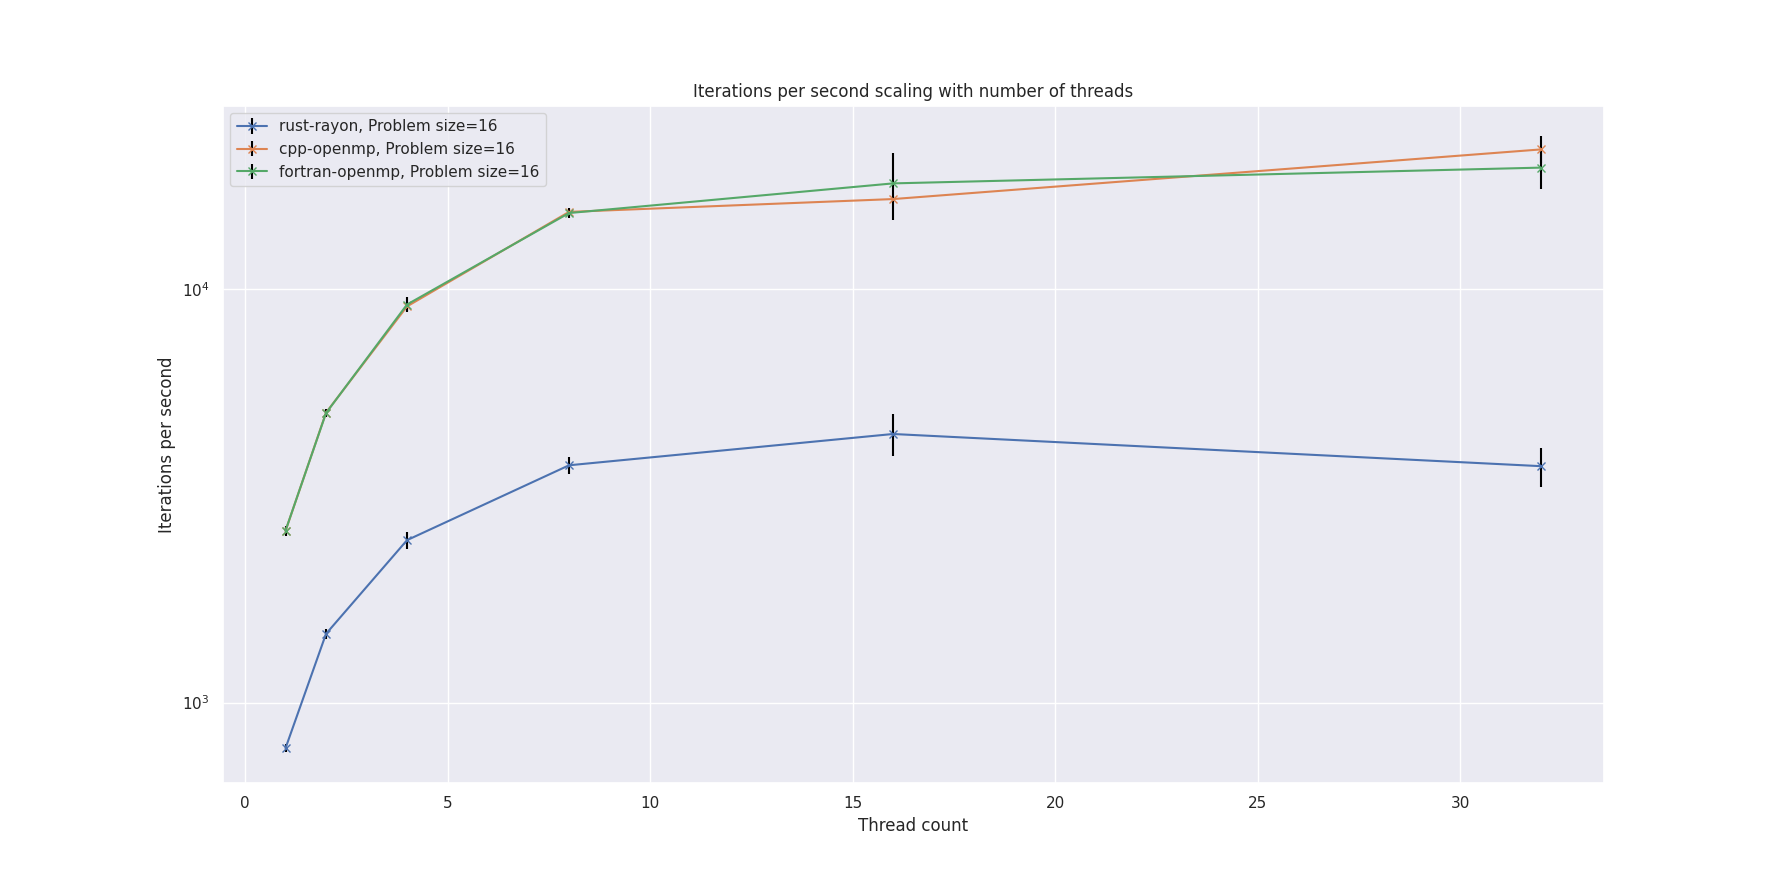
\includegraphics[width=\textwidth]{images/4_tooling/replication_study/replication_mine_4.png}
    \caption{A plot showing rate of iterations scaling with the number of threads used, replicated using HPC MultiBench.}
    \label{fig:replication_mine_4}
\end{figure}


The results of the replication trial broadly match those reported in the paper, except \ref{fig:replication_mine_4} for small mesh sizes, which could differ as a result of machine noise. The key take-away of this process is the degree to which the HPC MultiBench tool simplifies this critical process in the unbiased review of academic literature, turning a task which would take many hours to do manually into one which only takes about half an hour if the YAML file needs to be created, or just seconds if the YAML file is published with the results.

However, the utility of the HPC MultiBench tool is not limited to conducting replication trials -- it is also incredibly useful for conducting original experiments. However, replication trials best demonstrate the very high reduction in developer time as a result of the tool, by fixing the impact of experimental design.


\section{Industry review}
\label{sec:hpc-multibench-industry-review}

Once development of the HPC MultiBench tool was complete, meetings with two PhD candidates, Toby Flynn and Sam Curtis, both working in the High Performance and Scientific Computing Group at Warwick, were organised. These meeting served to review the tool, help understand how it fits into the existing landscape, and collect suggestions for future features.

In both meetings, the use case and a demonstration of the tool was presented. Toby commented that it ``sounds like a really good idea for seeing how things went'', and that ``anything I have done in the past I think I could do in the YAML file'', which confirms the use case and the abstraction provided by the YAML schema respectively. Sam commented that ``I would definitely use something like this'', and ``the problem you think exists definitely does'', similarly confirming the validity of the use case and usefulness of the tool.

In addition to this, there was discussion of future features which could improve the usefulness of the tool. This included first-class support for the \texttt{spack} package manager (similar to current support for module loads), the capability to average across results in a metric, and support for extending environment variables as well as overwriting them. In addition to this, the ongoing development to support plotting rooflines was received favourably, with Sam stating ``roofline plotting is one of the most painful things in HPC'', so tooling to simplify it is desirable.

\chapter{Performance}
\label{ch:performance} % 2000-2500 words

\textbf{This chapter is now complete - but wasn't in the first three chapter draft submission!}

As enumerated in the objectives summary section of the introduction \ref{ch:ssec:objectives-summary}, on of the three requirements for Rust's suitability as a language for High-Performance Computing is having a comparable performance to C++, one of the most commonly used languages in current usage.

This chapter provides an empirical assessment of the performance of the Rust translation of the HPCCG mini-app. As discussed in the background section introducing HPCCG \ref{ssec:hpccg}, this is representative of High-Performance Computing workloads, due to the design goals of Mantevo Suite mini-apps being representative of full applications to facilitate hardware-software co-design. We leverage this property to instead assess the Rust language's suitability for such workloads by comparing the performance of the Rust translation to the original C++ implementation.

This performance profiling will begin with the use of instrumentation tooling to identify hot-spots in source code, characterising the bottlenecks in the Rust and C++ compiled executables. This allows a direct comparison of compiled assembly, yielding a clear picture of ways in which the Rust language differs from C++. Then, the HPC MultiBench tool will be used to run and analyse direct measurements of the Rust and C++ codebases. This allows the characterisation and comparison of performance for strong and weak scaling, and parallelism approaches, along with the generation of roofline models.

\section{Profiling tools}
\label{sec:profiling-tools} % 500 words

Software profilers are a category of tools which are used to measure properties of running programs. They differ from static analysis tools, as they analyse programs dynamically as they run, usually through instrumentation inserted at compile time, rather than using the source code itself. Profilers are most often used to characterise the performance and memory usage of programs, and through instrumentation can identify ``hotspots'' -- code sections in the program which account for a disproportionate amount of the metric, such as overall runtime. This makes profilers useful for guiding optimisations, as engineering effort can be targeted at the portion of program which impacts performance most greatly.

Performance profilers can also be used to compare implementations of the same software in different languages. Comparing the  profiles of the programs on the same problem size can elucidate where one language loses performance over another, and give insights into key factors such as vectorisation and memory bandwidth utilisation.

We choose to use a variety of performance profilers, because some profilers provide many more metrics and analysis options, but typically at the expense of the simple and ergonomic user interface. As a result of this, we used \texttt{perf} for the majority of profiling tasks, as they provide a convenient command line interface for instrumentation statistical sampling. We also used the Intel\textregistered\ oneAPI\texttrademark\ suite of tools, including Intel\textregistered\ vTune\texttrademark\ and Intel\textregistered\ Advisor\texttrademark, as these provide a vast array of capabilities such as roofline analysis, but with a complex graphical-only interface.


\subsection{The \texttt{perf} profiler}
\label{ssec:perf-profiler}

\texttt{perf} is a performance analysis tool which has been part of the Linux kernel since the 2.6.31 release in 2009 \cite{PerfcountersAddedMainline}. It uses a ``git-like'' subcommand based command line interface  \cite{de2010new}, which allows it to perform many functionalities. The \texttt{record} subcommand uses a single kernel syscall to instrument statistical sampling or program performance, and the \texttt{report} subcommand presents an analysis of this recorded data.

The \texttt{perf} profiler was used throughout the translation process to identify hotspots in the code. The benefit of this process was two-fold. Firstly, it allowed manual performance-guided optimisation, allowing prioritisation of engineering effort to ensure the Rust implementation was a fair representation of the full extent of the languages capabilities when comparing it to C++. Secondly, the hotspots identified provided a strong insight into the parts of Rust programs that fall short of C++, which informs the assessment of the suitability of Rust for High-Performance computing applications.

% As discussed in the introduction
The Rust programming language places a strong focus on the prevention of undefined behaviour, including enforcing memory and thread safety. The key insight of the language was that many of these guarantees against undefined behaviour can be made at compile time, through the ownership model enforced by the borrow checker. However, there is not enough information at compile time to fully guarantee these characteristics. For example, creating a vector of a length provided by user input at run time is a common operation within many programs. However, if the programmer accesses this vector by a fixed index in the source code, the compiler cannot guarantee the indexing operation is within the bounds of this vector, since its size is not known until runtime. To avoid undefined behaviour, Rust checks the bounds of every indexing operations to guarantee that the index is not out of range, but this incurs a performance cost -- roughly doubling the time taken for vector indexing. To avoid this check in performance critical applications when the bounds are already guaranteed, Rust provides the \mintinline{rust}{get_unchecked} function, which does not perform the bound check. This performance cost can be seen through comparing \texttt{perf} reports when using the default bounds checked indexing in Figure \ref{fig:perf-checked}, against unchecked indexing in Figure \ref{fig:perf-unchecked}.

\begin{figure}[H]
    \centering
    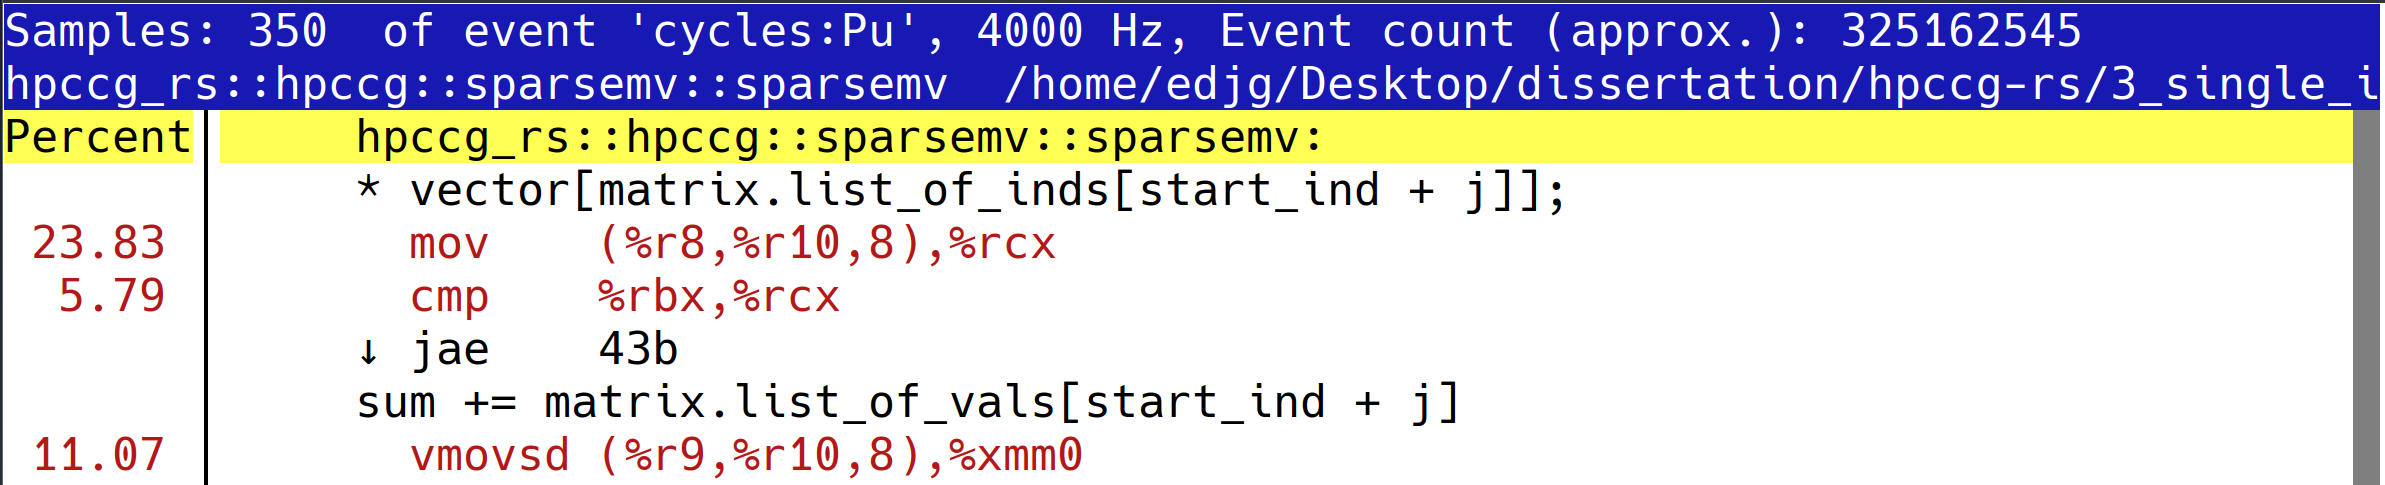
\includegraphics[width=0.95\textwidth]{images/5_performance/perf_checked_op.png}
    \caption{A screenshot of the \text{perf} report of a Rust translation of HPCCG using the default checked indexing.}
    \label{fig:perf-checked}
\end{figure}

\begin{figure}[H]
    \centering
    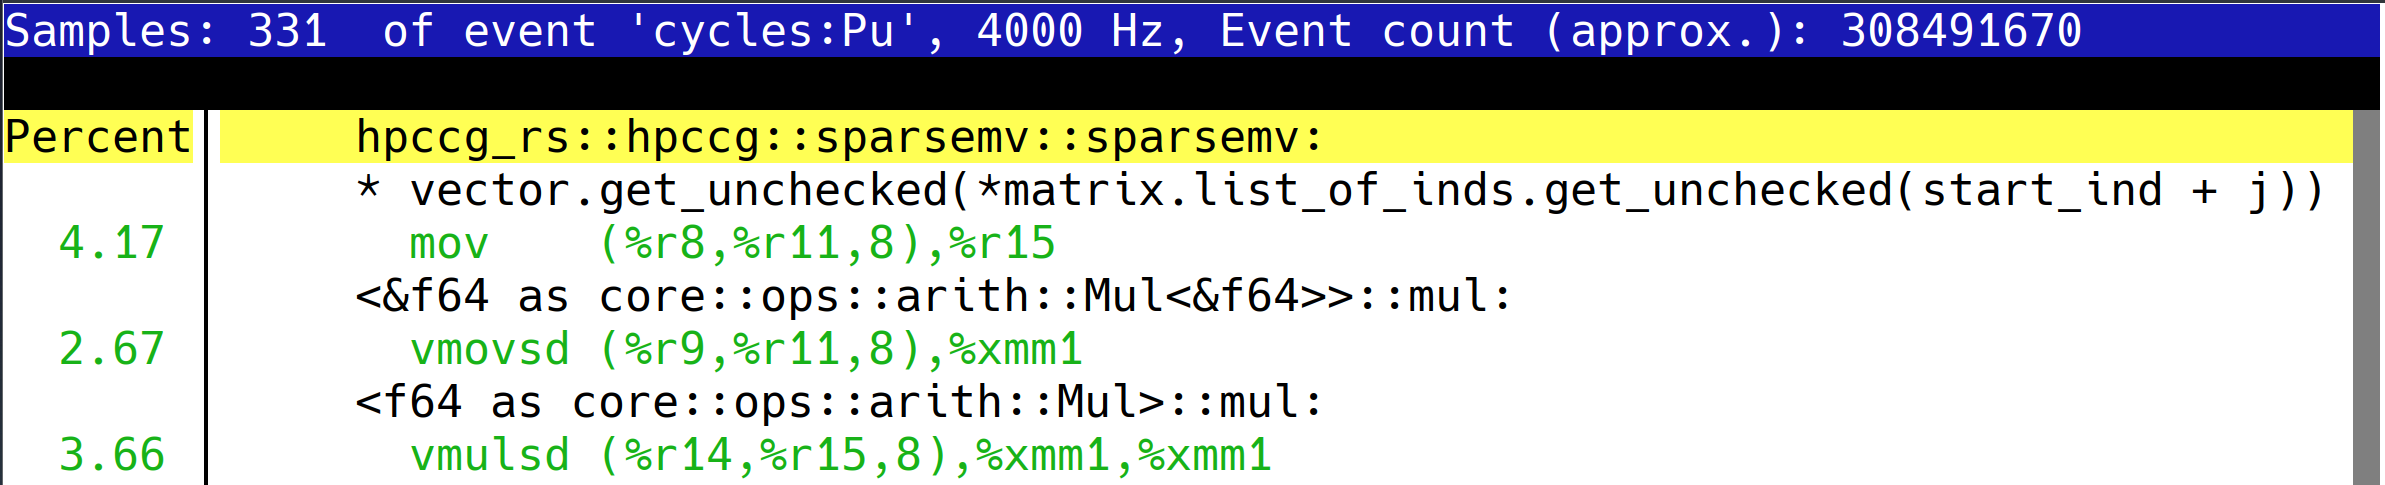
\includegraphics[width=0.95\textwidth]{images/5_performance/perf_unchecked_op.png}
    \caption{A screenshot of the \text{perf} report of a Rust translation of HPCCG using the unchecked indexing.}
    \label{fig:perf-unchecked}
\end{figure}

From these figures, we can see that the the bounds checking operation dominate the total runtime of the program, with $23.83 + 5.79 = 29.62$ percent of the runtime being taken up by the \mintinline{rust}{vector[matrix.list_of_inds[start_ind + j]]} operation in the bounds checked version, but only $4.17 + 2.67 + 3.66 = 10.5$ percent in the version without bounds checking. The empirical result of a $2.82\times$ speed-up for array indexing, a very common operation in High-Performance computing workloads, demonstrates the utmost importance of understanding and leveraging the full extent of the Rust language to be able to write performant software.

% Zero-cost abstractions
% iterators as a zero-cost abstraction? are they?

\subsection{The Intel\textregistered\ oneAPI\texttrademark\ suite}
\label{ssec:intel-advisor-profiler}
% Intel vTune Advisor
% Roofline model

\subsubsection{Roofline models}
\label{sssec:roofline-models}

% Introducing roofline models
In their seminal paper ``Roofline: an insightful visual performance model for multicore architectures'', Williams, Waterman and Patterson introduce the roofline model as a technique for simply characterising performance in complex systems \cite{williamsRooflineInsightfulVisual2009}. The model combines three metrics: Computational performance, memory bandwidth, operational intensity.

Computer hardware can be modelled as three components: execution units, data sources, and the interconnection between them. Computational performance measures how fast these execution units can process data in FLOP/s, and memory bandwidth measures the rate at which data can be transmitted across the interconnection in Bytes/s. As computational performance, memory bandwidth quantify hardware performance, operational intensity quantifies software performance. It refers to the average amount of data required per operation in a program, in FLOPS/byte. Rooflines are then drawn as, as shown in Figure \ref{fig:ert-roofline}, on a log-log axis, with the ``loft'' being a 45 degree line sloping up, and the ``ceiling'' a horizontal line.

\begin{figure}[H]
    \centering
    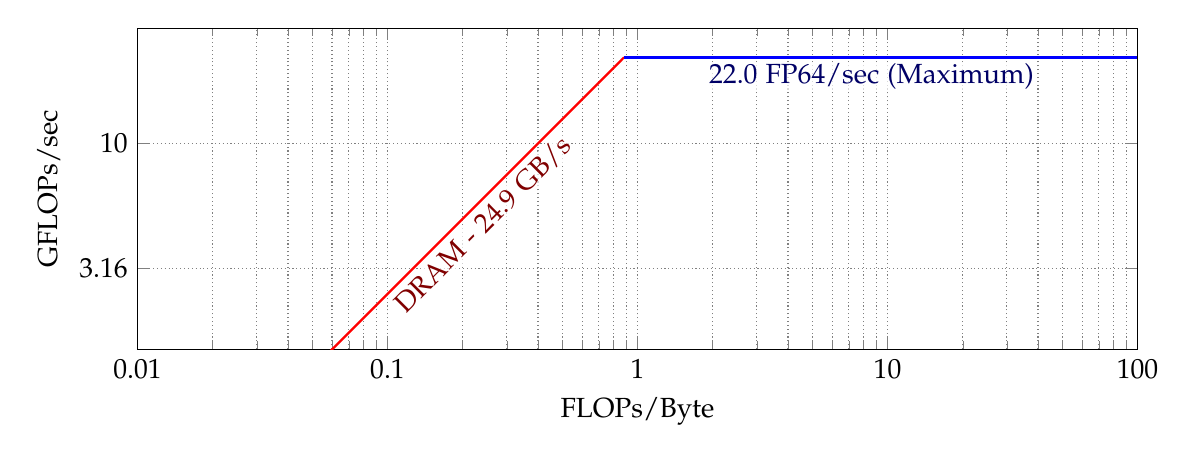
\begin{tikzpicture}
      \pgfplotsset {
        scale only axis,
        axis equal image,
        width=5in,
        /pgf/number format/1000 sep={},
        /tikz/maxline/.style={blue, thick, no marks},
        /tikz/memline/.style={red, thick, no marks},
        /tikz/maxlabel/.style={blue!40!black, right, fill=white, fill opacity=0.7, text opacity=1.0, rounded corners=2pt, inner sep=0.5pt},
        /tikz/memlabel/.style={red!50!black, rotate=45, right, fill=white, fill opacity=0.7, text opacity=1.0, rounded corners=2pt, inner sep=0.5pt}
      }
    
      \def\Xmin{1.000000e-02}
      \def\Xmax{1.000000e+02}
    
      \begin{loglogaxis}[
        grid=both,
        grid style={black!50, densely dotted},
        xlabel= FLOPs/Byte,
        ylabel= GFLOPs/sec,
        xmin=\Xmin,
        xmax=\Xmax,
        ymin=1.500000e+00,
        ymax= ,
        log ticks with fixed point
        ]
    
        \node[maxlabel] at (axis cs: 1.9000000e+00,1.8448000e+01) {22.0 FP64/sec (Maximum)};
        \node[memlabel] at (axis cs: 1.1036459e-01,2.1571047e+00) {DRAM - 24.9 GB/s};
        \addplot[memline, domain=(\Xmin:8.8336673e-01)] {2.4950000e+01*x};
        \addplot[maxline, domain=(8.8336673e-01:\Xmax)] {2.2040000e+01};
    
      \end{loglogaxis}
    \end{tikzpicture}
    \caption{A roofline graph, modified from the output of the Empirical Roofline Tool \cite{EmpiricalRooflineTool}.}
    \label{fig:ert-roofline}
\end{figure}

The paper summarises the roofline model as ``set[ing] an upper bound on performance of a kernel depending on the kernel’s operational intensity. If we think of operational intensity as a column that hits the roof, either it hits the flat part of the roof, meaning performance is compute-bound, or performance is ultimately memory-bound'' \cite{williamsRooflineInsightfulVisual2009}. This allows the easy identification of where optimisations for the kernel might be possible.

Later, Ilic, Pratas and Sousa proposed a modification to the roofline model to include information about cache bandwidths in their paper ``Cache-aware Roofline model: Upgrading the loft'' \cite{ilic_cache-aware_2014}. This adds multiple ``lofts'', as the memory bandwidth of caches are higher that of main memory. In addition to this, SIMD instructions can result in additional ceilings, as the peak attainable computational performance of vectorised instructions is necessarily higher.

Roofline models are a powerful technique to simply characterise the bottlenecks in software. As such, tools such as the Intel\textregistered\ Advisor can be used to generate them.

\subsubsection{Generating rooflines with Intel\textregistered\ Advisor}
\label{sssec:roofline-generation-intel-advisor}

The Intel\textregistered\ Advisor tool is part of the Intel\textregistered\ oneAPI\texttrademark\ suite. Intel describes it as ``a design and analysis tool for developing performant code'' \cite{DesignCodeParallelism}, and one of the functionalities it provides is generating roofline plots. This is commonly done using its graphical user interface, but it is possible to also generate plots as minified HTML files from the command line. Listing \ref{listing:roofline-generation} shows the sequence of commands required to generate the roofline plots for an executable. 

\begin{listing}[H]
    \begin{minted}[linenos,breaklines]{bash}
advisor -collect roofline -project-dir ./ -- ./test_HPCCG
advisor --report=roofline --project-dir=./ --report-output=./roofline.html
    \end{minted}
    \caption{The commands required generate roofline models from the command line.}
    \label{listing:roofline-generation}
\end{listing}

Using these plots, we can characterise whether the computational kernels are memory or compute bound in each language, which gives an insight into how their performance can be improved. Roofline plots can be applied to multi-threaded and distributed workloads, however assuming a uniform processor architecture, the degree of parallelism does not significantly impact whether the kernels are computer or memory bound. As such, roofline plots for multi-threaded and distributed workloads are not included here, as they are not relevant and often less clear. Figure \ref{fig:cpp-roofline} shows the roofline plot for the C++ implementation of HPCCG, and Figure \ref{fig:rust-roofline} for plot for the Rust translation.

\begin{figure}[H]
    \centering
    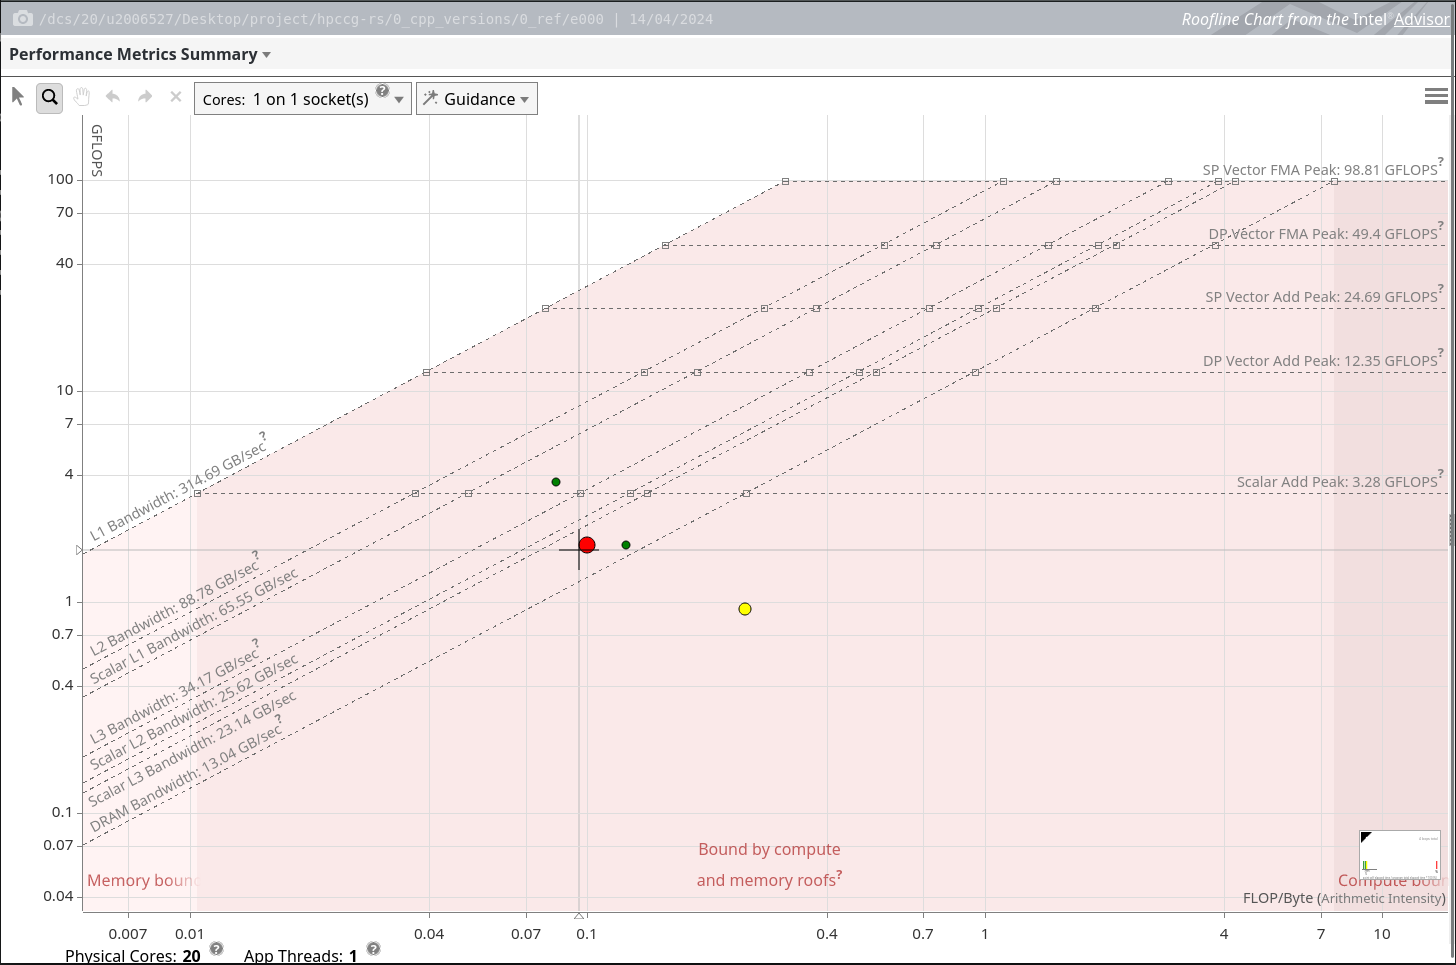
\includegraphics[width=\textwidth]{images/5_performance/rooflines/cpp_roofline.png}
    \caption{A roofline diagram generated by Intel\textregistered\ Advisor\ showing the performance of the C++ implementation of HPCCG.}
    \label{fig:cpp-roofline}
\end{figure}

\begin{figure}[H]
    \centering
    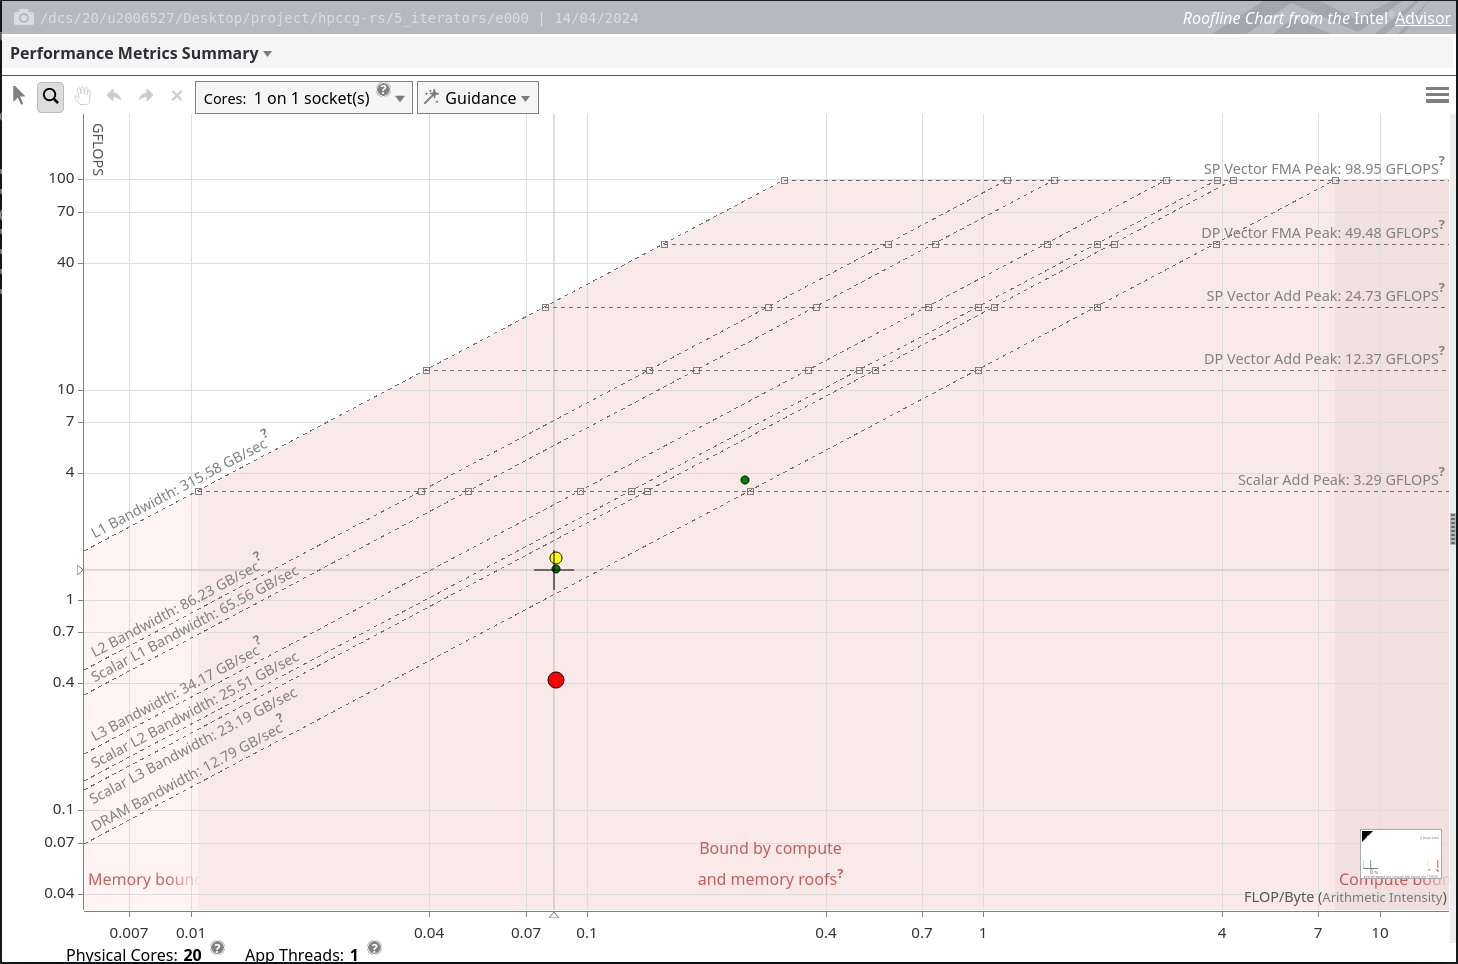
\includegraphics[width=\textwidth]{images/5_performance/rooflines/rust_roofline.png}
    \caption{A roofline diagram generated by Intel\textregistered\ Advisor\ showing the performance of the Rust translation of HPCCG.}
    \label{fig:rust-roofline}
\end{figure}

From these plots, we can see that both the C++ and Rust implementations appear to be mostly memory bound, with the DRAM bandwidth limiting the performance of the functions. Since these rooflines were generated on very small meshes of size $25 \times 25 \times 25$, to avoid overloading Intel\textregistered\ Advisor, we can see that some of the kernels for both implementations are within the cache section of the plot, as the mesh data is small enough to be fully included in cache memory. We can also see that the \texttt{waxpby}, shown by the upper green dot in Figure \ref{fig:cpp-roofline}, in the C++ is amenable to vectorisation, and as such is able exceed the scalar compute roofline. Finally, the locations of the kernels across the plots differ fairly significantly, indicating the different software loads have different performance characteristics across the two languages.

Overall, C++ has both a higher arithmetic intensity and rate of floating point operations, which indicates it is able to make better use of the compute hardware it runs on. As a result of this, we expect direct measurements of the C++ program to have slightly higher performance.

In addition to using the Intel\textregistered\ Advisor, HPC MultiBench supports plotting rooflines for performance characterisation at a glance as part of larger test plans. It parses JSON data generated by the Empirical Roofline Tool \cite{EmpiricalRooflineTool} to generate the ceilings, and the Likwid toolkit \cite{RRZEHPCLikwid2024} to calculate operational intensity and performance. An example of this is shown in Figure \ref{}.

% TODO: HPC MultiBench figure here

This figure confirms the statement that the mini-app is memory bound, and shows that employing multi-threading techniques allows implementations to better leverage the hardware they are run on.

Performance profilers provide a very powerful tool for identifying and optimising away hotspots in running programs. However, profilers are typically best suited for measuring many performance metrics in a fixed configuration, such as with a set number of processor threads and MPI ranks. To assess Rust's suitability for High-Performance Computing, we only needed a few metrics such as runtime and FLOPs, but wanted to measure how these varied across a wide range of metrics, with statistical confidence. As a result of this, we switched to a direct measurement approach driven by the HPC MultiBench tool, which was designed for this purpose.

\section{Direct measurement}
\label{sec:direct-measurement} % 2000 words

For Rust to be a suitable language for High-Performance Computing workloads, it must have a comparable performance across both a range of parallelism approaches, from serial execution to multi-threading and message passing across a compute cluster, and for large data volumes. To assess this, we used a wall clock approach to time the original C++ and the translated Rust implementations of HPCCG across a variety of problem sizes, and with a variety of thread counts and MPI sizes.

\subsection{Experimental methodology}
\label{ssec:experimental-methodology}

% In the intro to the book Performance Tuning of Scientific Applications, David Bailey suggests nine guidelines for presenting performance results without misleading the reader. Paraphrasing only slightly, these are: 

The experiments are fully defined by the YAML configuration files for the HPC MultiBench tool, providing extremely strong reproducibility characteristics. The salient features this provides include driving the programs across a range of inputs and configurations, along with supporting re-runs to give statistical confidence in the results.

For all experiments in this results section, the programs are run five times. The slowest run is then always discarded as an outlier, due to the possibility of machine noise or network instability for MPI workloads.

The original HPCCG implementation provides a number of different timers which measure the computational kernels. These include clock ticks, resource usage, wall time, and MPI timing intrinsics. By default, resource usage is used for serial and threaded compilations, and MPI timing intrinsics when MPI is used. However, the resource usage timer records the sum of the times for each thread. As a result of this, the \texttt{-DWALL} compiler flag was set to use the wall time. This allows representative comparisons to be made, as otherwise Rust may record faster times for short runs as a result of Rayon's work-stealing threading model. Finally, the UNIX \texttt{time} utility was also used to assess the total runtime including matrix setup, rather than just computational kernel runtimes.

On Kudu, 60GB of RAM was used, and on Avon 40GB was used, due to hardware limitations. During development, smaller RAM sizes were used, resulting in significantly degraded performance as a result of the mesh sizes exceeding allocated RAM, resulting in memory thrashing \cite{pattersonHennessyComputerOrganisationArchitecture}. To mitigate this, these very large RAM sizes were used, which guarantees thrashing does not occur since the mesh size does not exceed the amount of memory used, even for mesh sizes of $400 \times 400 \times 400$.


\subsubsection{Reproducibility}
\label{sssec:parallelism-approaches-reproducibility}

The raw data files and test plan YAML files for the results are available in the base and \texttt{\_test\_plan} directories of the \texttt{hpccg-rs-kudu-results} and \texttt{hpccg-rs-avon-results} repositories for the two compute systems respectively. Listing \ref{listing:serial-data-interactive} shows the command to launch the interactive user interface for the Kudu and Avon test plans respectively. When run locally, this allows the aggregation and analysis of the generated results to be viewed. If run on the appropriate batch computer system, the test benches can be re-run with the ``Run Test Plan'' button.

\begin{listing}[H]
    \begin{minted}[linenos]{bash}
# For the DCS Kudu batch compute system
poetry run python3 -m hpc_multibench \
    -y generated_results/hpccg-rs-kudu-results/_test_plans/parallelism.yaml \
    interactive
# For the SCRTP Avon batch compute system
poetry run python3 -m hpc_multibench \
    -y generated_results/hpccg-rs-avon-results/_test_plans/parallelism.yaml \
    interactive
    \end{minted}
    \caption{The commands required to interactively view and re-run the performance experiments for the parallelism approaches test benches.}
    \label{listing:serial-data-interactive}
\end{listing}

This yet again shows the power of the HPC MultiBench tool beyond the example use case shown in section \ref{ssec:hpc-multibench-replication-study}, as the experimental results presented in the previous section can easily be reviewed and even re-run, using a single command.


\subsubsection{System specifications}
\label{sssec:system-specifications}

During the course of experimentation, three different compute resources were used: Athena, the author's personal laptop; Kudu, the DCS batch compute system; and Avon, the Warwick SCRTP High-Performance Computing resource. Athena was used for the translation effort and initial testing, but not for any experimental results. However, since tests during the development process informed decisions made during the design process, its system specifications are relevant. Kudu was used for the majority of testing and the project presentation demo, as it is easy to access and has short queue times. Avon was used for later tests to confirm results, and for very large tests which exceeded Kudu's capacity.

Allow for reproducibility of the reported test data, the hardware specifications for the machines used as follows, with additional information about the machines listed in Appendix \ref{sec:hardware-specifications} for completeness. For Kudu and Avon, \texttt{slurm} is used to dispatch jobs, so the commands are run from within a \texttt{slurm} job to be representative of the compute nodes rather than the login nodes of the cluster.

% TODO: Convert to table?
\begin{itemize}
    \item Athena has a \texttt{Intel(R) Core(TM) i7-8565U CPU @ 1.80GHz} with eight logical cores.
    \item Kudu has a \texttt{Intel(R) Xeon(R) CPU E5-2660 v3 @ 2.60GHz} with 40 logical cores.
    \item Avon has a \texttt{Intel(R) Xeon(R) Platinum 8268 CPU @ 2.90GHz} with 48 logical cores.
\end{itemize}

The software versions used for benchmarking across the three systems are enumerated in the following table:

% TODO: Add compiler flags
\begin{table}[H]
    \caption{A table showing the software versions across the three compute resources.}
    \label{table:perfTools}
    \begin{tabular}{|p{0.24\linewidth}||p{0.2\linewidth}|p{0.2\linewidth}|p{0.2\linewidth}|}
    \hline
    \textbf{Software name} & \textbf{Athena} & \textbf{Kudu} & \textbf{Avon} \\
    \hline\hline
    Operating system & EndeavourOS 2023.03.26 & Rocky Linux 8.9                & CentOS Linux 8.4.2105          \\\hline
    Linux kernel     & 6.6.24-1-lts                     & 4.18.0-513.18.1. el8\_9.x86\_64 & 4.18.0-305.88.1. el8\_4.x86\_64 \\\hline
    rustc            & 1.73.0                           & 1.75.0                         & 1.75.0                         \\\hline
    clang            & 17.0.6                           & 16.0.6                         & 13.0.1                         \\\hline
    g++              & 13.2.1                           & 9.2.0                          & 11.3.0                         \\\hline
    OpenMP           & 4.5                              & 4.5                            & 4.5                            \\\hline
    rayon            & 1.8.0                            & 1.8.0                          & 1.8.0                          \\\hline
    OpenMPI          & 5.0.2                            & 4.0.5                          & 4.1.4                          \\\hline
    rs-mpi           & 0.7.0                            & 0.7.0                          & 0.7.0                          \\\hline
    \end{tabular}
\end{table}


\subsection{Strong scaling}
\label{ssec:strong-scaling}

Patterson and Hennessy define strong scaling as ``measuring the speed-up [due to parallelisation] while keeping the problem size fixed'' \cite{pattersonHennessyComputerOrganisationArchitecture}. This can be measured by recording the wall clock time taken for a fixed problem, whilst varying the degree of parallelisation, given by number of threads or MPI ranks. It can be used to show how adding more computational resources to a problem effects its performance. An ideal speedup due to parallelisation would decrease execution time linearly with the number of resources added. However, programs with a serial component cannot achieve this ideal speed-up as a corollary of Amdahl's law \cite{amdahlsLaw}:

\begin{equation}
    S = \frac{1}{f + \frac{1-f}{P}}
\end{equation}

Where $f$ denotes the proportion of execution time spent on the serial component, $P$ the degree of parallelisation, and $S$ the total speedup of the system as a result of parallelisation. For problems well-suited to parallelisation, we expect to see strong speedup approach the upper bound for performance following Amdahl's law.

In the context of the HPCCG mini-app, strong scaling can be measured for each of the two parallelism approaches, shared memory with multi-threading and distributed memory with MPI. Comparing the scaling properties of these approaches between the C++ implementation and Rust translation can then yield insight into how the application may perform for very large workloads. Figures \ref{fig:strong_scaling_threaded} and \ref{fig:strong_scaling_mpi} compare the strong scaling characteristics of the total runtimes of the C++ and Rust implementations. The mesh sizes for these benchmarks taken from testing scripts for strong scaling in the original HPCCG repository, ranging from $64 \times 64 \times 1024$ to $64 \times 64 \times 32$ reducing exponentially on the z axis. These mesh sizes are comparatively small, which can be seen in the high impact of serial overhead in these results.

% TODO: Could cut raw runtime plots if they aren't interesting?
\begin{figure}[H]
    \centering
    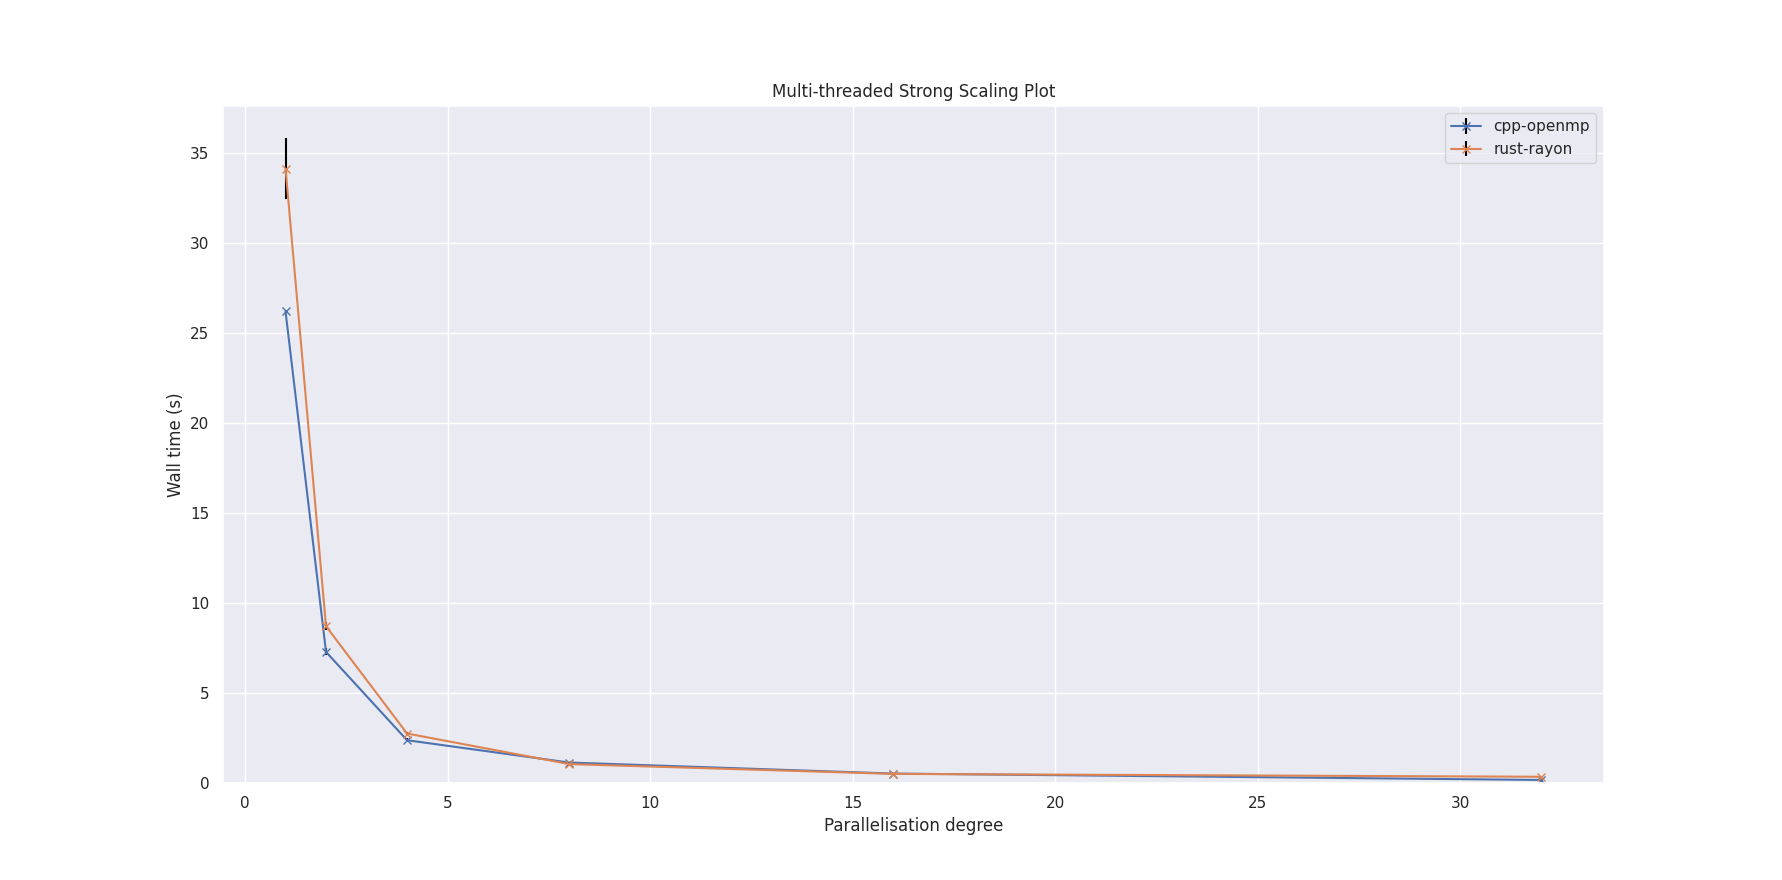
\includegraphics[width=\textwidth]{images/5_performance/scaling/strong_scaling_threaded.png}
    \caption{A line plot comparing the strong scaling runtimes of the C++ and Rust implementations of HPCCG using shared memory parallelism.}
    \label{fig:strong_scaling_threaded}
\end{figure}

\begin{figure}[H]
    \centering
    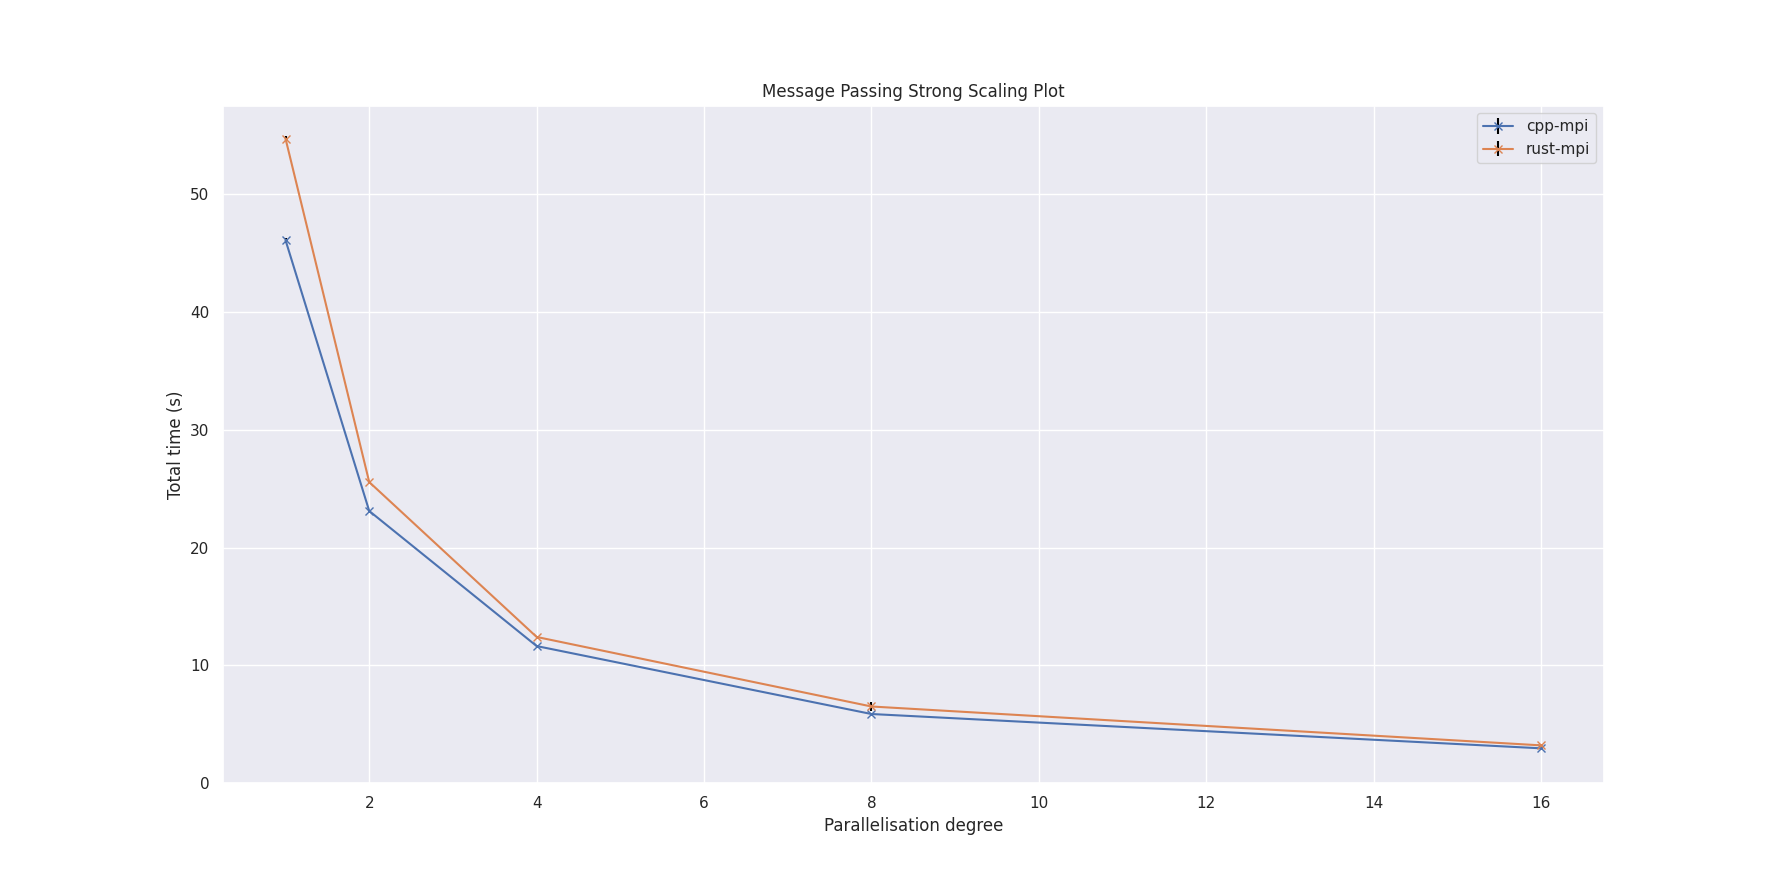
\includegraphics[width=\textwidth]{images/5_performance/scaling/strong_scaling_mpi.png}
    \caption{A line plot comparing the strong scaling speedups of the C++ and Rust implementations of HPCCG using distributed memory parallelism.}
    \label{fig:strong_scaling_mpi}
\end{figure}

Leveraging the HPC MultiBench framework we can also easily plot the speedup of the two approaches, rather than the raw runtimes. The speedup plots for the C++ and Rust implementations are shown in Figures \ref{fig:strong_scaling_speedup_threaded} and \ref{fig:strong_scaling_speedup_mpi} respectively.

\begin{figure}[H]
    \centering
    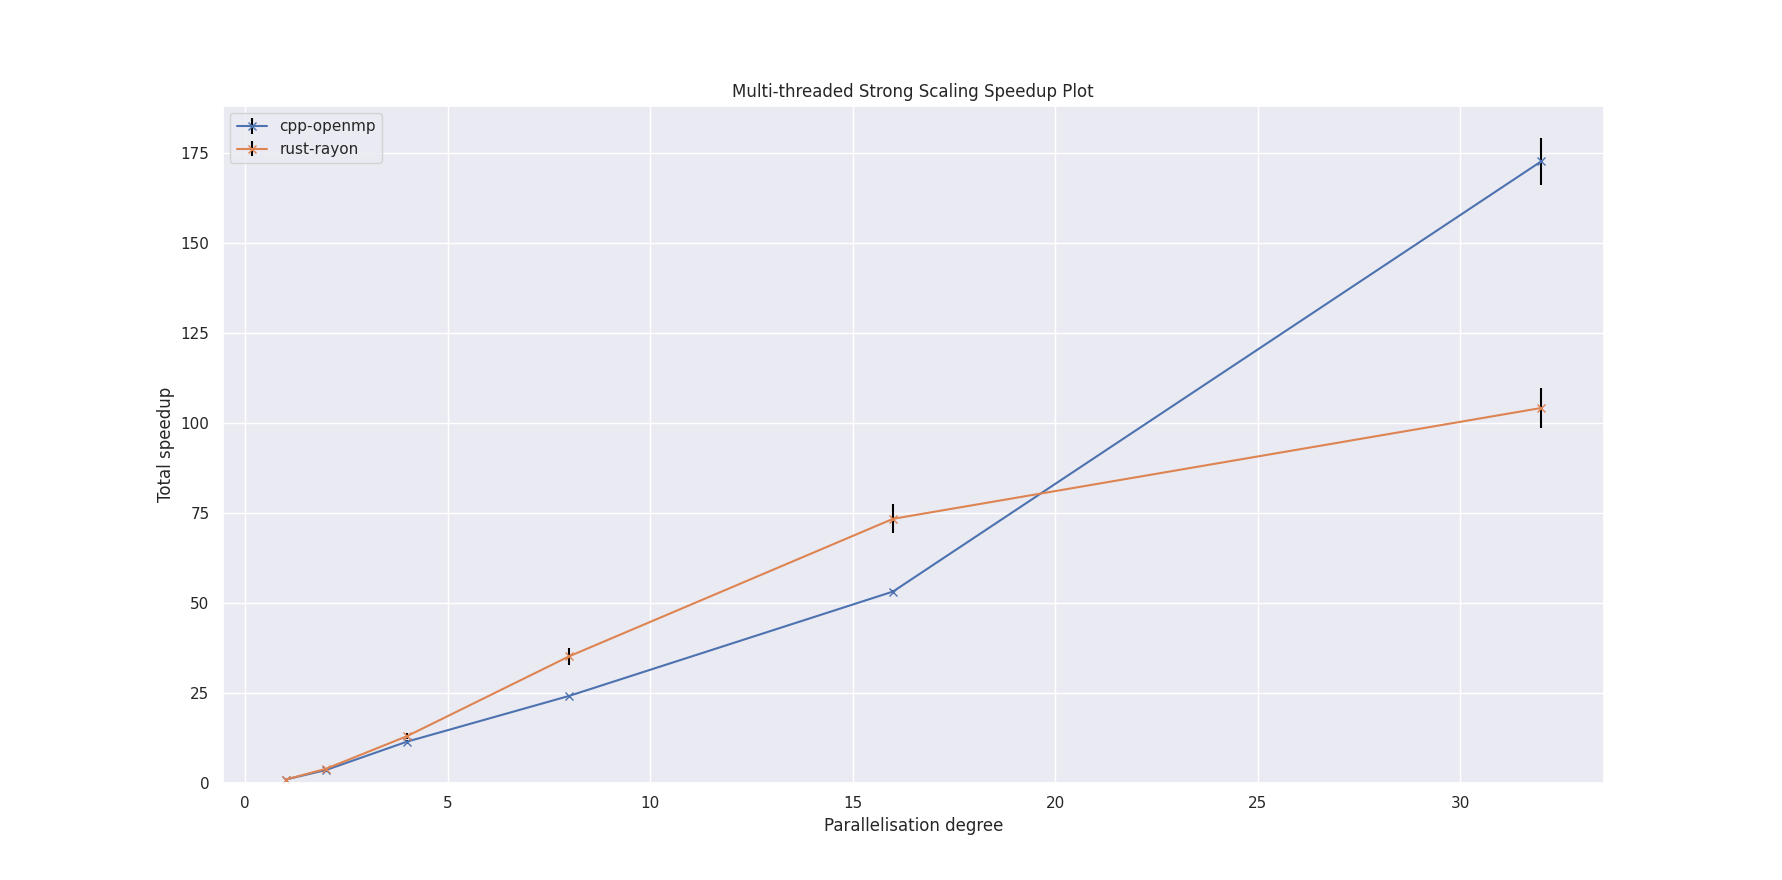
\includegraphics[width=\textwidth]{images/5_performance/scaling/strong_scaling_speedup_threaded.png}
    \caption{A line plot comparing the strong scaling speedups of the C++ and Rust implementations of HPCCG using shared memory parallelism.}
    \label{fig:strong_scaling_speedup_threaded}
\end{figure}

\begin{figure}[H]
    \centering
    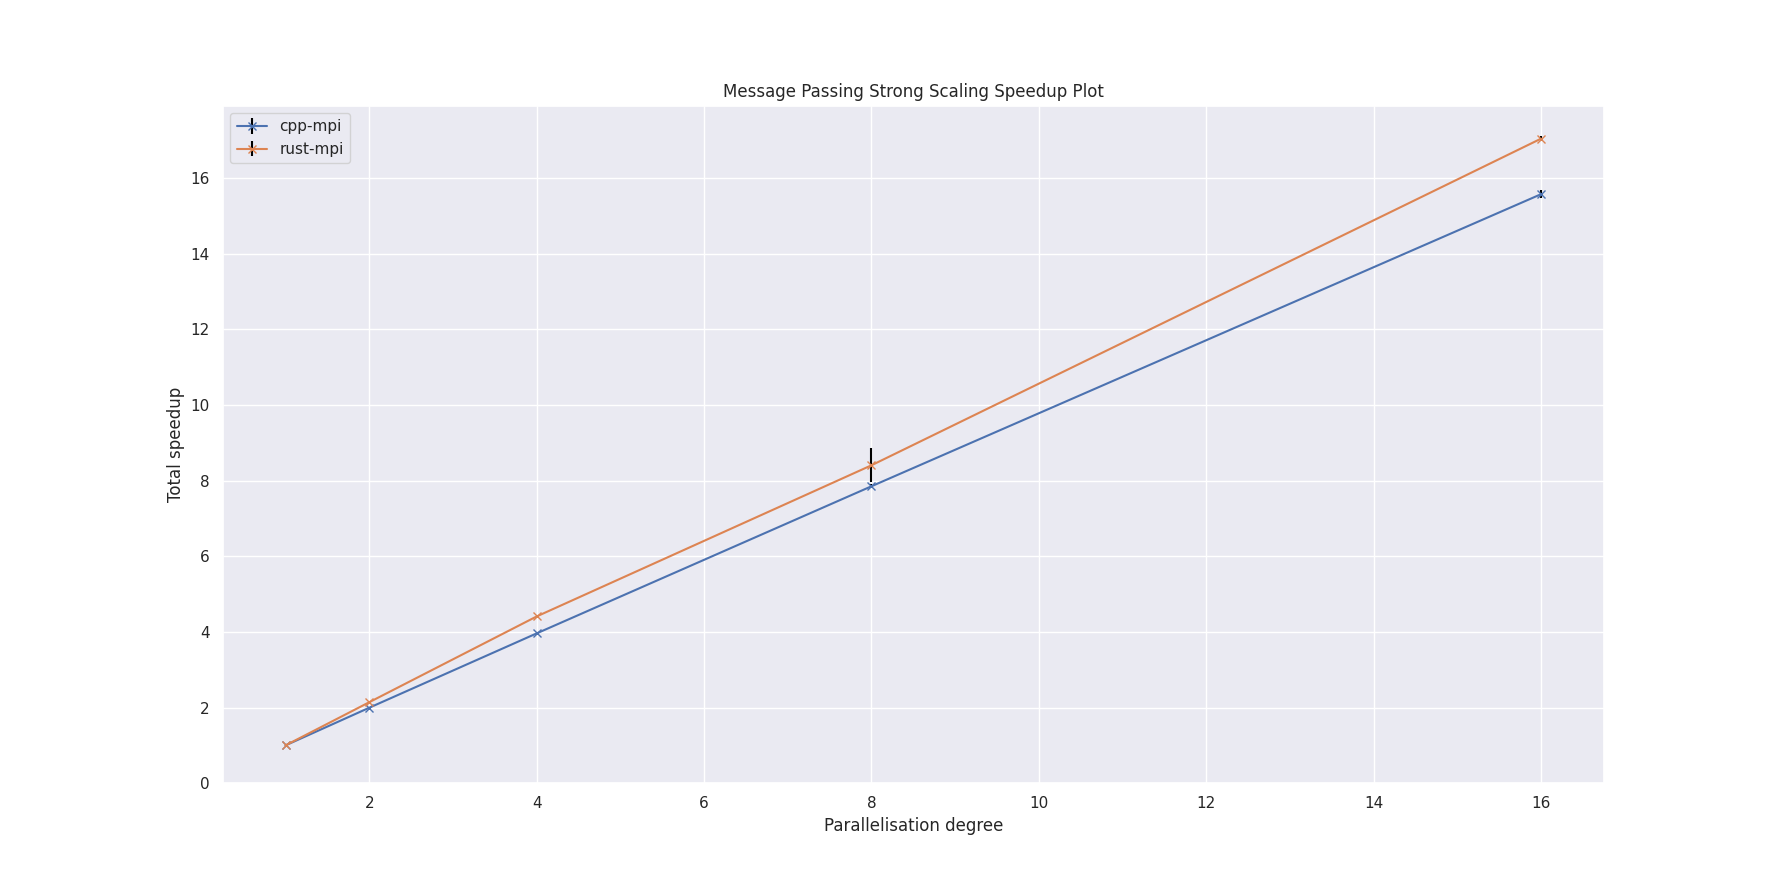
\includegraphics[width=\textwidth]{images/5_performance/scaling/strong_scaling_speedup_mpi.png}
    \caption{A line plot comparing the strong scaling runtimes of the C++ and Rust implementations of HPCCG using distributed memory parallelism.}
    \label{fig:strong_scaling_speedup_mpi}
\end{figure}

% TODO: Could easily separate and compare kernels, but already over the word count...

Examining the plots showing speedup rather than raw runtime allow better understanding of the trends in program performance. From these speedup plots, we can see that for the small meshes tested Rust's threading model through Rayon of work stealing appears to scale less well than OpenMP, outside of the range of experimental error. However, this is likely due to significant impact the serial overhead of setting up the thread pool has on the total execution time for such small workloads. For MPI, we can see an almost ideal strong scaling speedup of two very straight lines. Again, the speedup of Rust is slightly lower, which is likely due to overhead incurred in invoking the MPI bindings.

In summary, we can see that both the C++ and Rust implementations strongly scale similarly, with both being close the theoretical limitation of Amdahl's law. This evidence of similar strong scalability provides confidence in the suitability of Rust for High-Performance Computing workloads, which require this property to effectively leverage clustered compute resources.

\subsection{Weak scaling}
\label{ssec:weak-scaling}

Patterson and Hennessy define weak scaling as ``measuring the speed-up while keeping the problem size fixed'' \cite{pattersonHennessyComputerOrganisationArchitecture}. This can be measured by recording the wall clock time taken, whilst varying the problem size at the same rate as the varying the degree of parallelisation, given by number of threads or MPI ranks. Since the workload grows with the number of resources added, ideal weak scaling is when the execution time remains constant as both factors are increased.

Unlike strong scaling, we cannot apply Amdahl's law to characterise weak scaling, since it assumes a fixed problem size. However, this extended case of variable problem size was characterised in 1988 in Gustafson's paper ``Re-evaluating Amdahl's law'' \cite{gustafsonReevaluatingAmdahlLaw1988}. Gustafson's law estimates the speedup, $S$ as a result of parallelisation in terms of the number of processors $N$, and the fractions of time executing the parallel and serial parts of the program, $p$ and $s$ respectively:

\begin{align}
    S &= s + p \times N \\
      &= N + (1 - N) \times s
\end{align}

From the above equation we can see that for ideal weak scaling to occur, the serial component of the program must remain constant as the degree of parallelism is increased. In real-world applications, we expect this to not be the case, as higher degrees of parallelism often incur higher serial costs, such as handling increased communication for MPI workloads, or overhead from spawning threads for multi-threaded ones.

% Weak scaling applied to HPCCG
In the context of HPCCG, as with strong scaling, weak scaling can again be measured for single-node (multi-threading only) and multi-node (multi-threading and message passing). Figures \ref{} and \ref{} compare the results of the C++ and Rust implementations for weak scaling across single-node and multi-node approaches.

As with strong scaling, weak scaling can be assessed for both parallelism approaches in the context of the HPCCG mini-app. Figures \ref{fig:weak_scaling_threaded} and \ref{fig:weak_scaling_mpi} compare the strong scaling characteristics of the total runtimes of the C++ and Rust implementations. The mesh sizes for these benchmarks are again taken from testing scripts for weak scaling in the original HPCCG repository, with the problem size fixed as $64 \times 64 \times 64$, which is again comparatively small.
% NOTE: This sounds weird to have the problem size fixed, but is consistent with the testing scripts (https://github.com/Mantevo/HPCCG/blob/master/weakScalingRunScript), and exhibits the expected behaviour???

% TODO: Could cut raw runtime plots if they aren't interesting?
\begin{figure}[H]
    \centering
    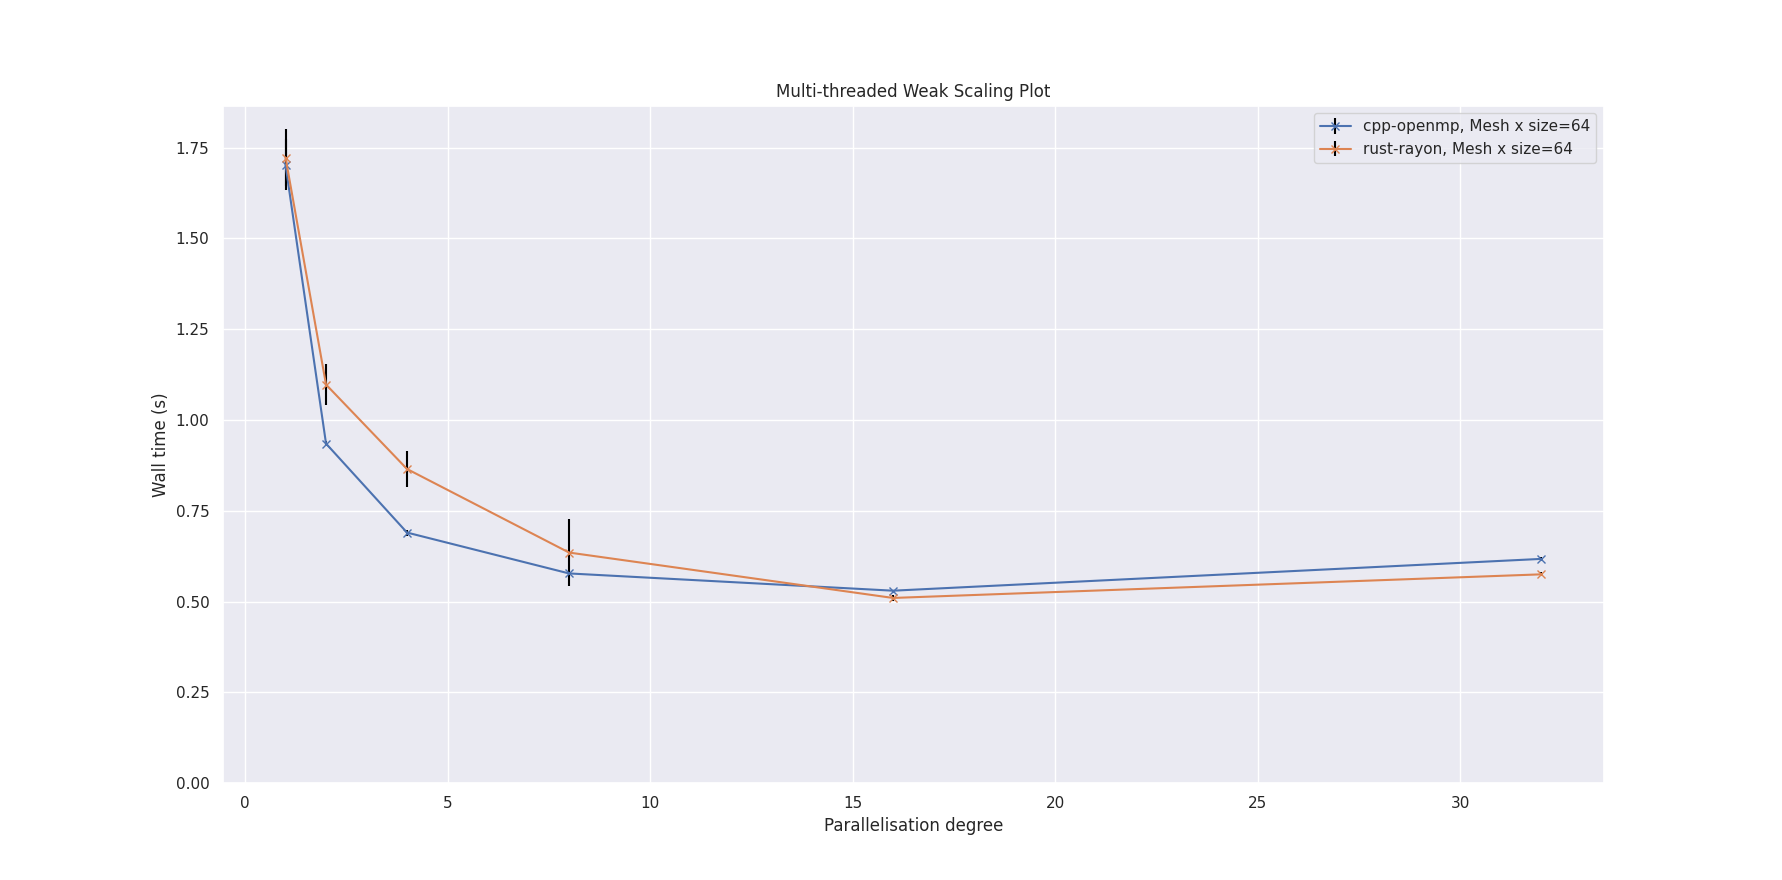
\includegraphics[width=\textwidth]{images/5_performance/scaling/weak_scaling_threaded.png}
    \caption{A line plot comparing the weak scaling runtimes of the C++ and Rust implementations of HPCCG using shared memory parallelism.}
    \label{fig:weak_scaling_threaded}
\end{figure}

\begin{figure}[H]
    \centering
    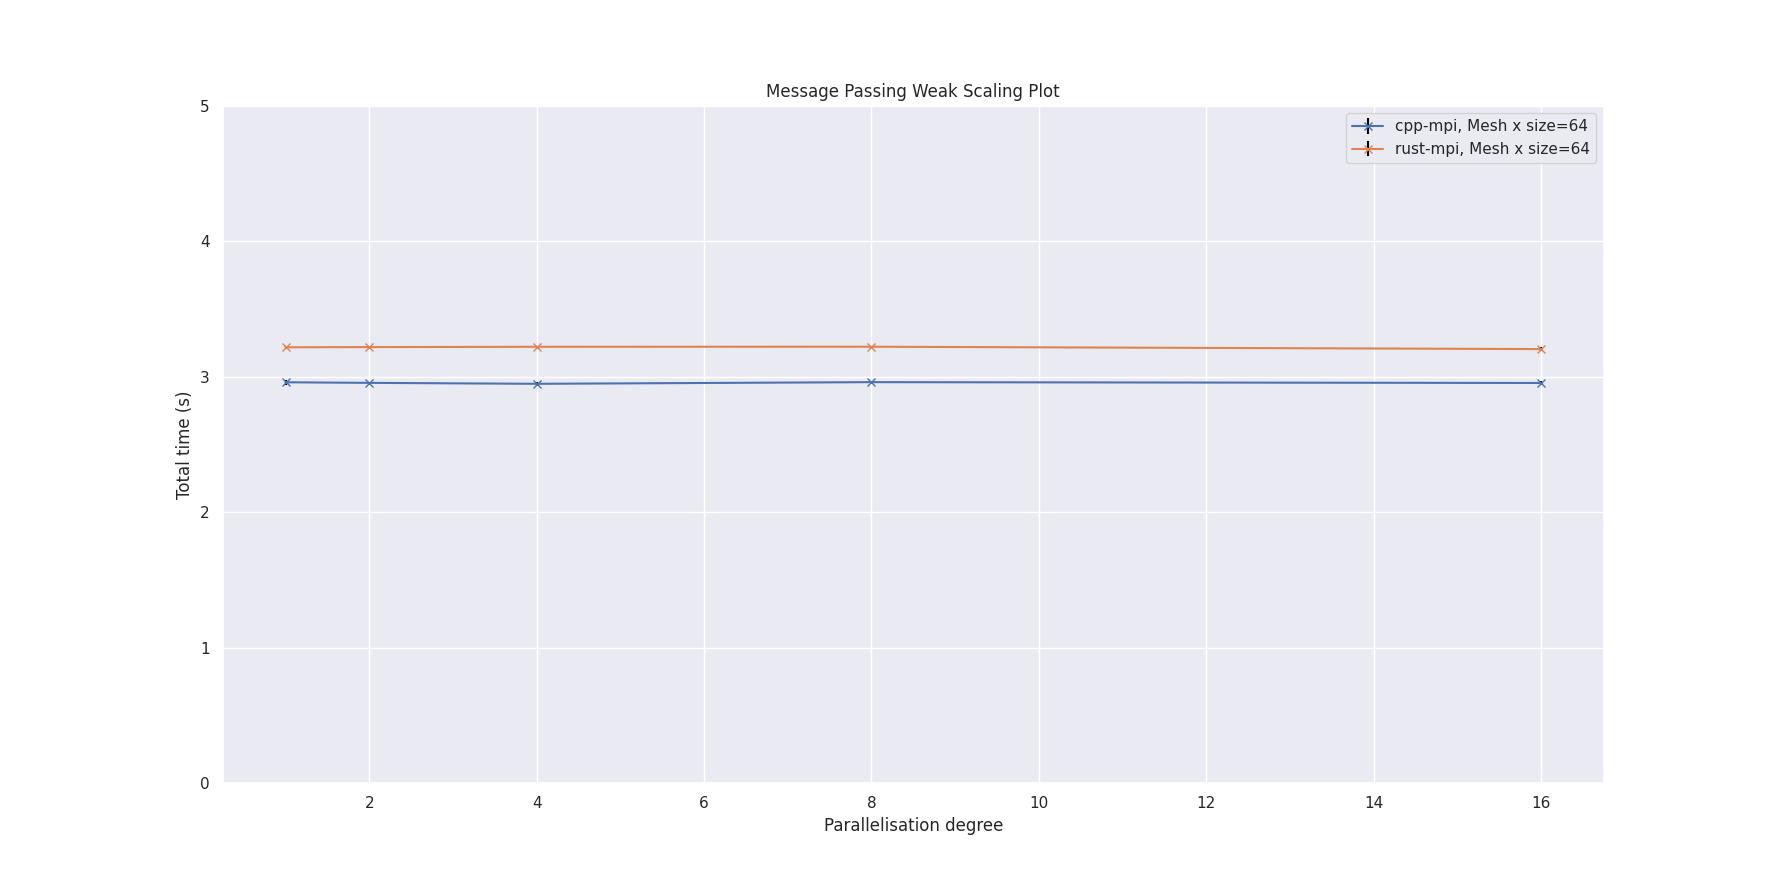
\includegraphics[width=\textwidth]{images/5_performance/scaling/weak_scaling_mpi.png}
    \caption{A line plot comparing the weak scaling speedups of the C++ and Rust implementations of HPCCG using distributed memory parallelism.}
    \label{fig:weak_scaling_mpi}
\end{figure}

Again, we can leverage the HPC MultiBench framework to plot the speedup of the two approaches, rather than the raw runtimes. The speedup plots for the C++ and Rust implementations are shown in Figures \ref{fig:weak_scaling_speedup_threaded} and \ref{fig:weak_scaling_speedup_mpi} respectively.

\begin{figure}[H]
    \centering
    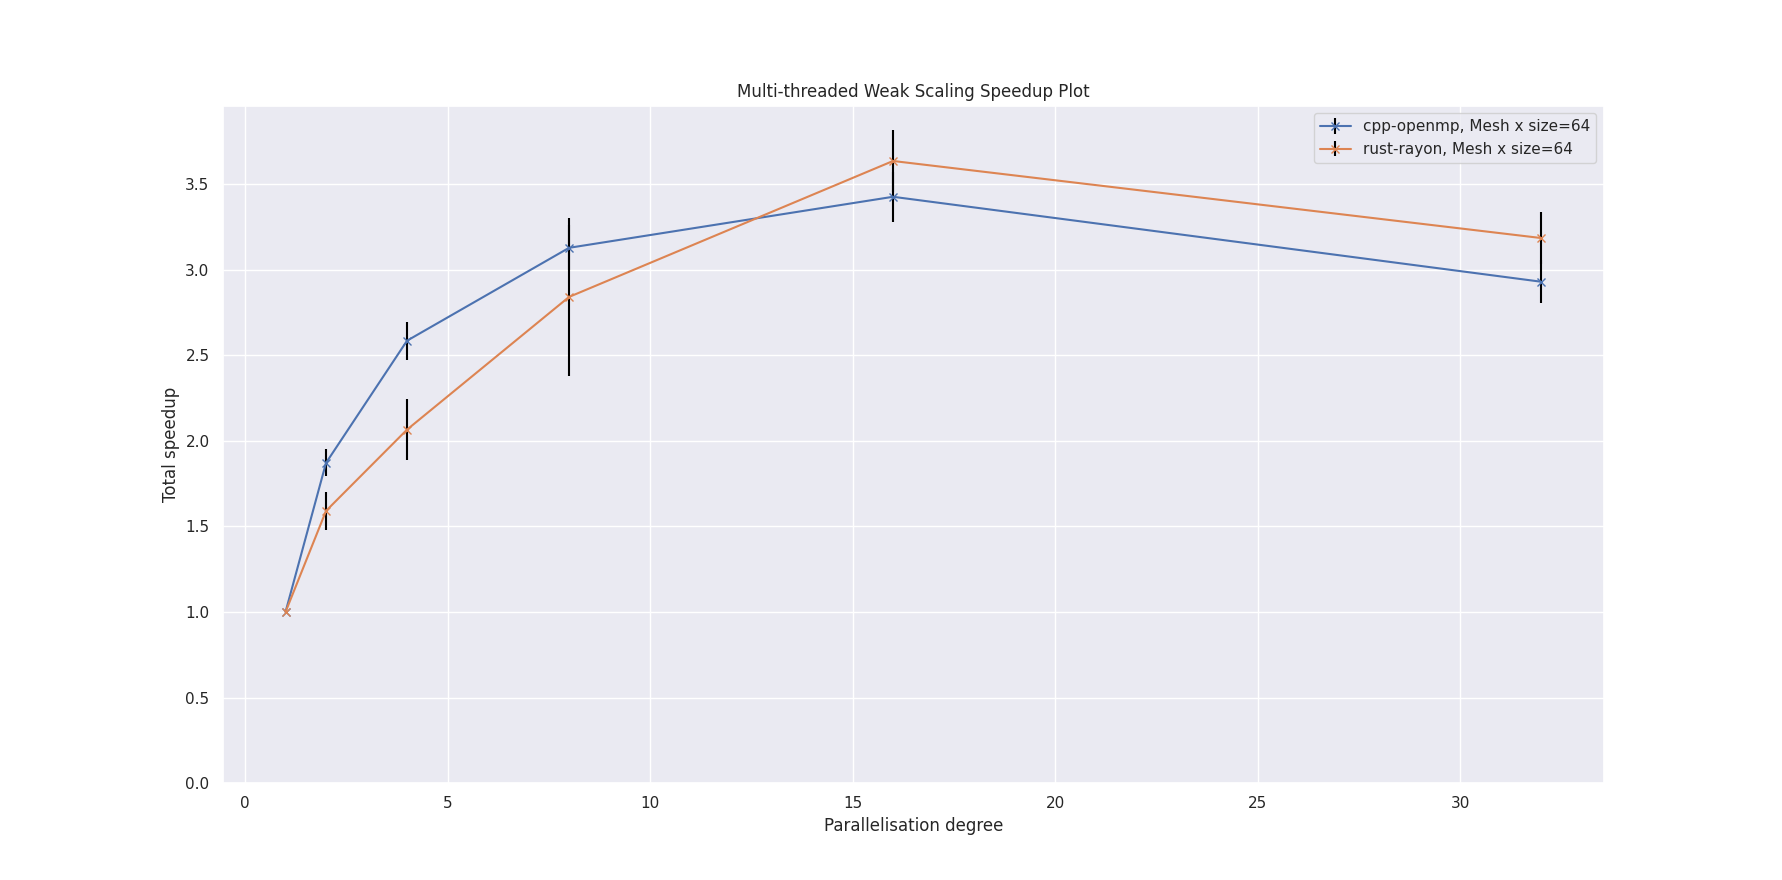
\includegraphics[width=\textwidth]{images/5_performance/scaling/weak_scaling_speedup_threaded.png}
    \caption{A line plot comparing the weak scaling speedups of the C++ and Rust implementations of HPCCG using shared memory parallelism.}
    \label{fig:weak_scaling_speedup_threaded}
\end{figure}

\begin{figure}[H]
    \centering
    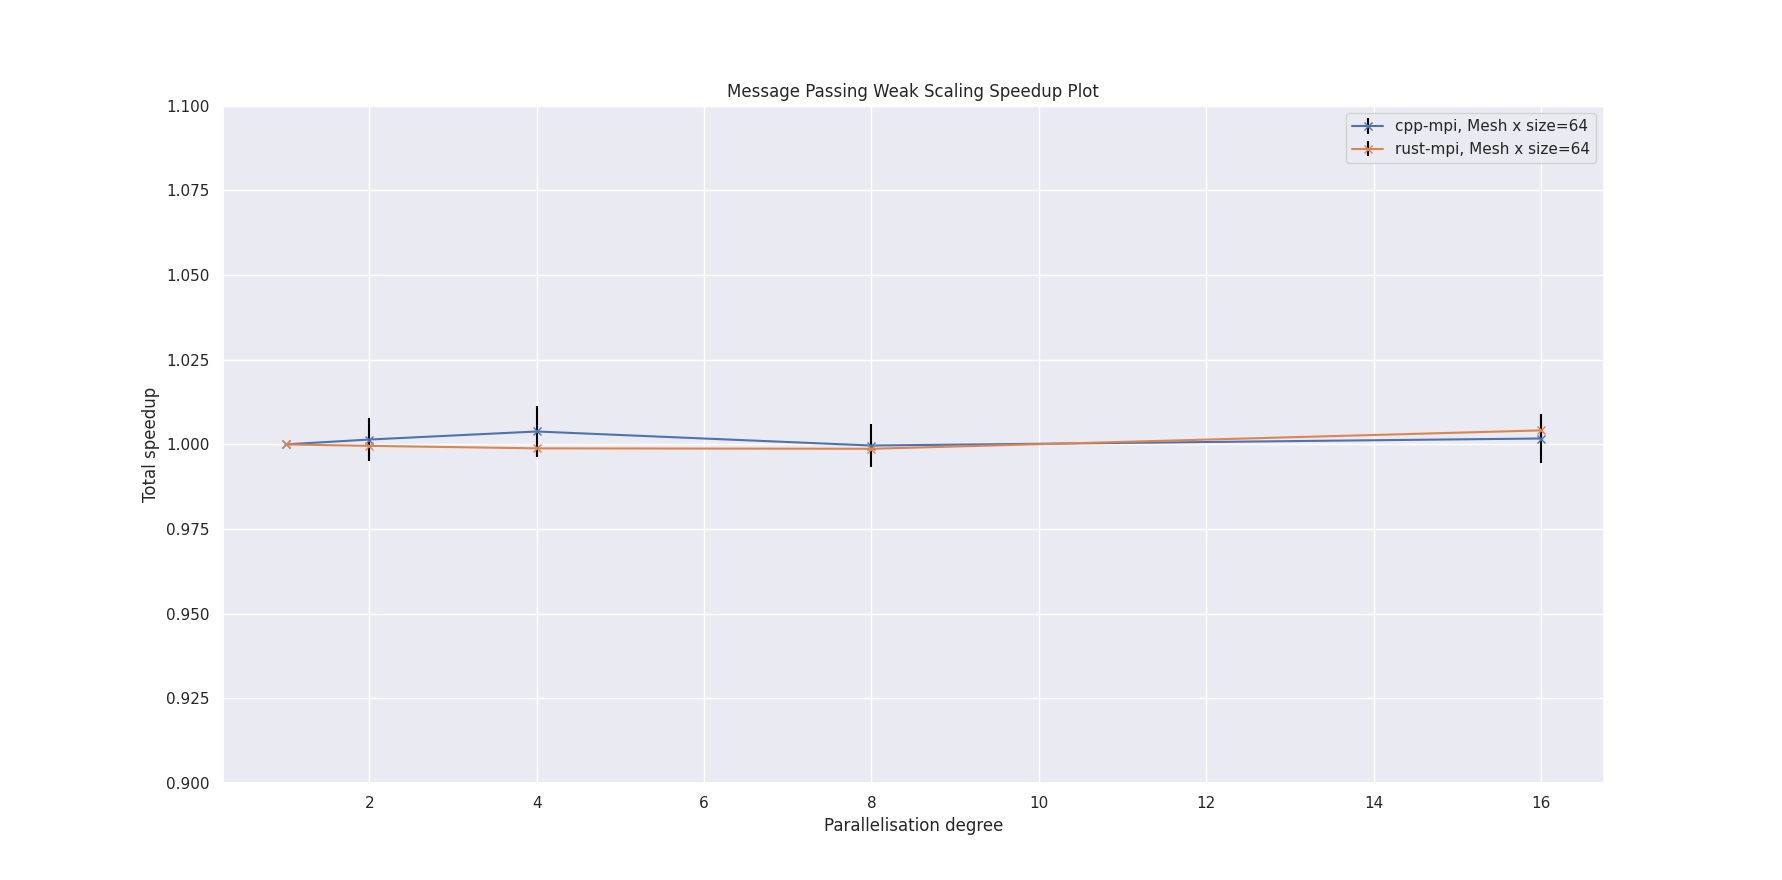
\includegraphics[width=\textwidth]{images/5_performance/scaling/weak_scaling_speedup_mpi.png}
    \caption{A line plot comparing the weak scaling runtimes of the C++ and Rust implementations of HPCCG using distributed memory parallelism.}
    \label{fig:weak_scaling_speedup_mpi}
\end{figure}

As with strong scaling, the speedup plots most effectively show the trends in program performance. The weak scaling trends of the multi-threaded approach are surprising, as the ideal result is a flat line, as seen in the message passing approach. This is likely because the serial overhead of setting up threading for very small thread counts dominates the runtime for small meshes, as a corrolary of Amdahl's law. In addition to this, the speedup trends back down for high thread counts, which could be due to the mesh being insufficiently large to effectively divide work between the threads. The weak scaling speedup of the message passing approach is very consistent across the two languages, with the Rust and C++ implementations being within experimental uncertainty of each other. This is likely because Rust is invoking the same MPI implementation that C++ uses, albeit through bindings.

In summary, we can see that both the C++ and Rust implementations weakly scale similarly, with both parallelism approaches following the same trends across the languages. This evidence of similar weak scalability again provides confidence in the suitability of Rust for High-Performance Computing workloads, which require this property to effectively leverage clustered compute resources.




\subsection{Parallelism approaches}
\label{ssec:parallelism-approaches}

% TODO: cite (same as background)
In modern High-Performance Computing systems, the majority of performance is achieved through parallelism. As a result of this, for Rust to be suitable for use in High-Performance Computing workloads, it must be able to achieve parallel compute performance similar to that of currently used languages, like C++. This section provides an empirical analysis of the performance of Rust as compared with C++ for increasingly parallel workloads, from serial as a reference to shared memory parallelism through multi-threading and distributed memory parallelism through message passing.

\subsection{Serial execution}
\label{ssec:multi-threaded}

Before exploring various parallelism approaches, it is important to measure a point of reference, in the form of serial execution of the program. In addition to just being a point of reference, the performance serial execution itself is an important metric. Almost program leveraging parallelism will have serial sections, and even if these are very short they can take up a significant proportion of a programs runtime for highly parallel programs, by Amdahl's law \cite{amdahlsLaw}. As a result of this, an empirical assessment comparing the performance of Rust with C++ workloads is highly relevant to the suitability of Rust for High-Performance Computing.

To assess serial performance, we ran the C++ and Rust executables over a range of mesh sizes, from $100 \times 100 \times 100$ to $300 \times 300 \times 300$, incrementing each axis size by $50$ each time. We expect the performance to scale with the total size of the mesh, which is the cube of the edge size. For the serial tests, all runs were conducted on a single node in the compute cluster, with a single task per node, and exclusive use of that node to reduce machine noise from other processes. As with all tests, 60GB of RAM was used on Kudu, and 40GB was used on Avon, to avoid memory thrashing for large mesh sizes, and performance is measured as wall time through the UNIX \texttt{time} utility. The results of these experiments are shown in Figures \ref{fig:1_serial_line} and \ref{fig:2_serial_line_relative} for Kudu, and \ref{fig:2_serial_line_relative_avon} on Avon.

\begin{figure}[H]
    \centering
    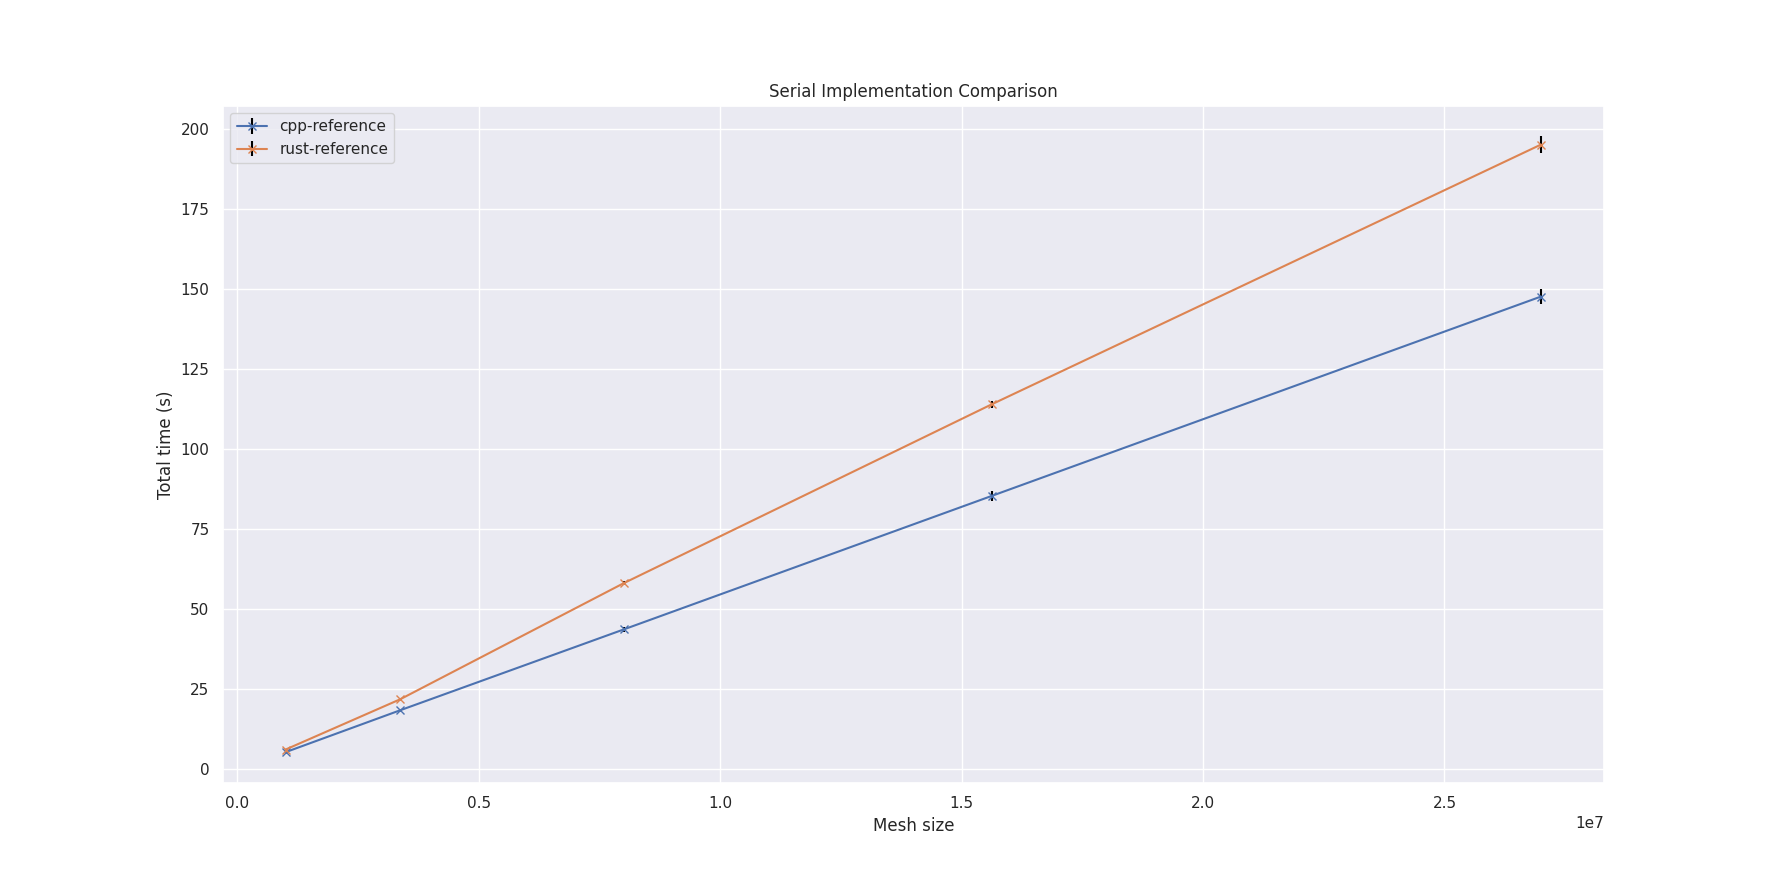
\includegraphics[width=\textwidth]{images/5_performance/parallelism/1_serial_line.png}
    \caption{A line plot comparing the total wall times for the Rust and C++ implementations of HPCCG, on the Kudu batch compute system.}
    \label{fig:1_serial_line}
\end{figure}

\begin{figure}[H]
    \centering
    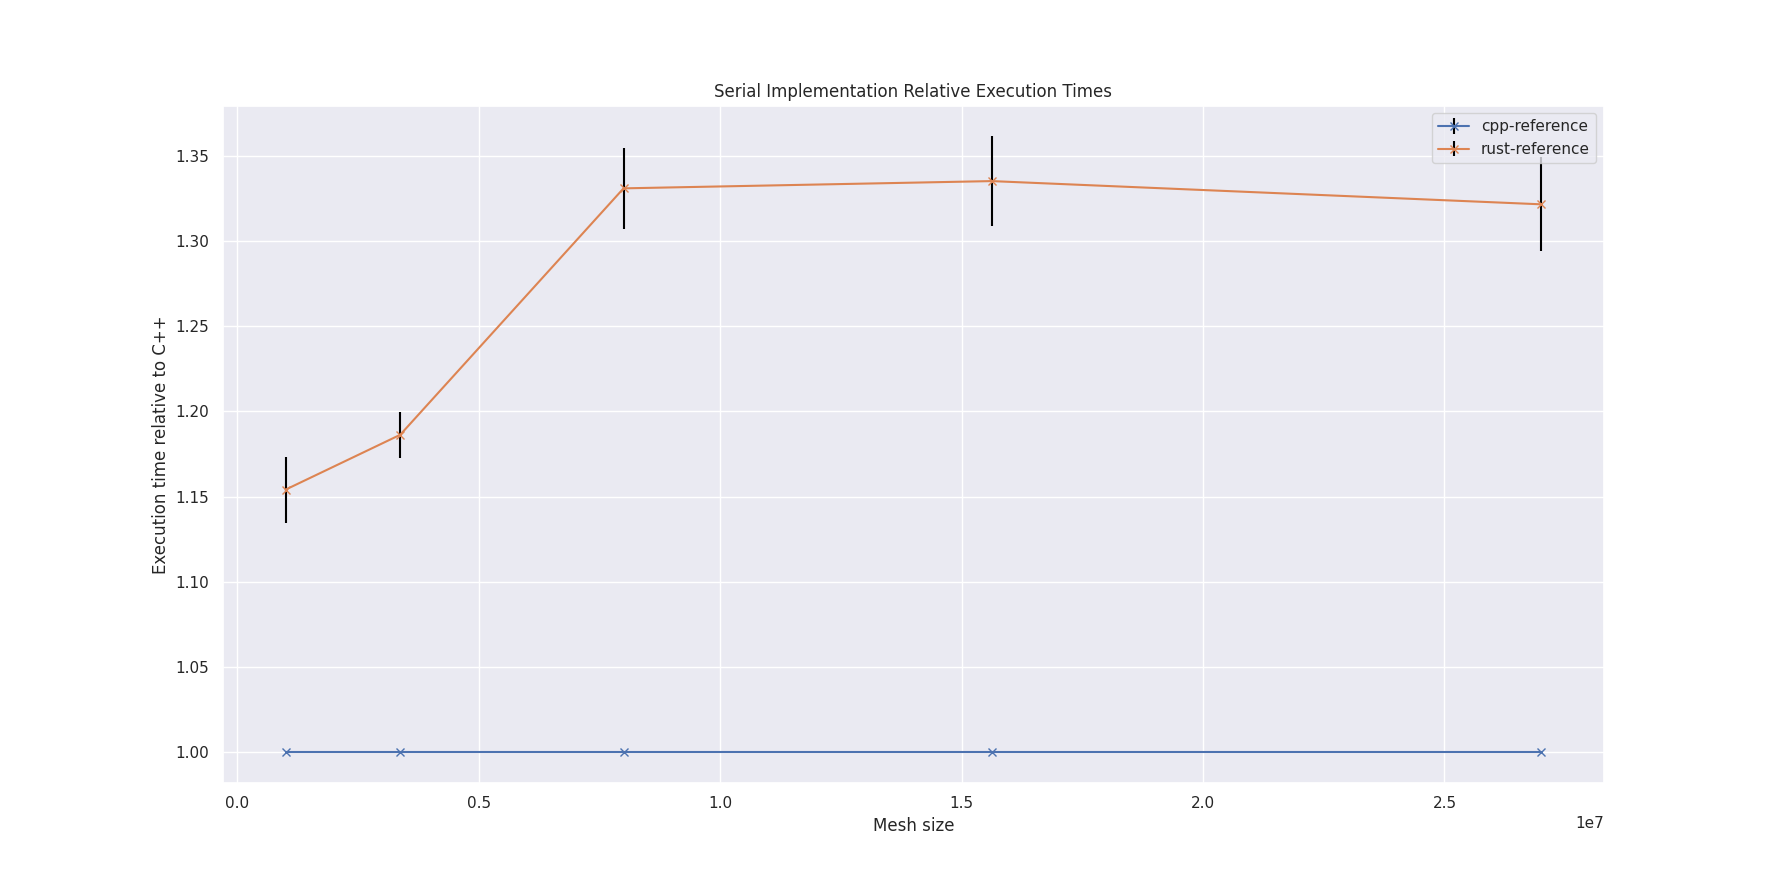
\includegraphics[width=\textwidth]{images/5_performance/parallelism/2_serial_line_relative.png}
    \caption{A line plot comparing the total wall times relative to the C++ implementation of HPCCG, on the Kudu batch compute system.}
    \label{fig:2_serial_line_relative}
\end{figure}

\begin{figure}[H]
    \centering
    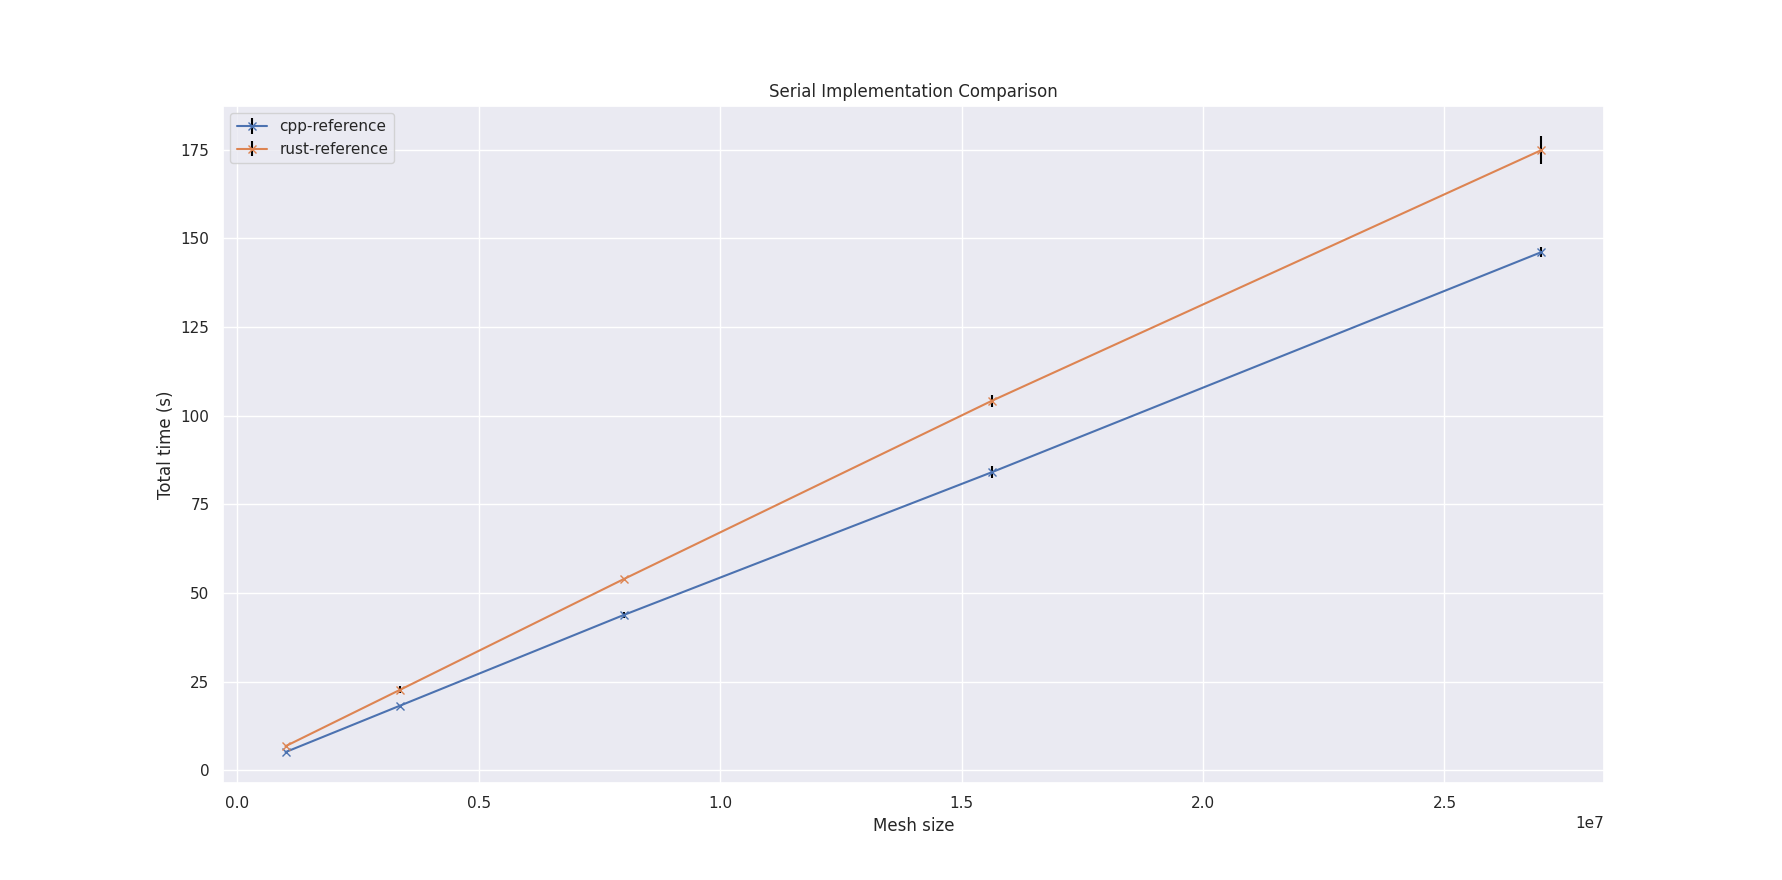
\includegraphics[width=\textwidth]{images/5_performance/parallelism/1_serial_line_avon.png}
    \caption{A line plot comparing the total wall times across all computational kernels for the Rust and C++ implementations of HPCCG, on the Avon batch compute system.}
    \label{fig:1_serial_line_avon}
\end{figure}

\begin{figure}[H]
    \centering
    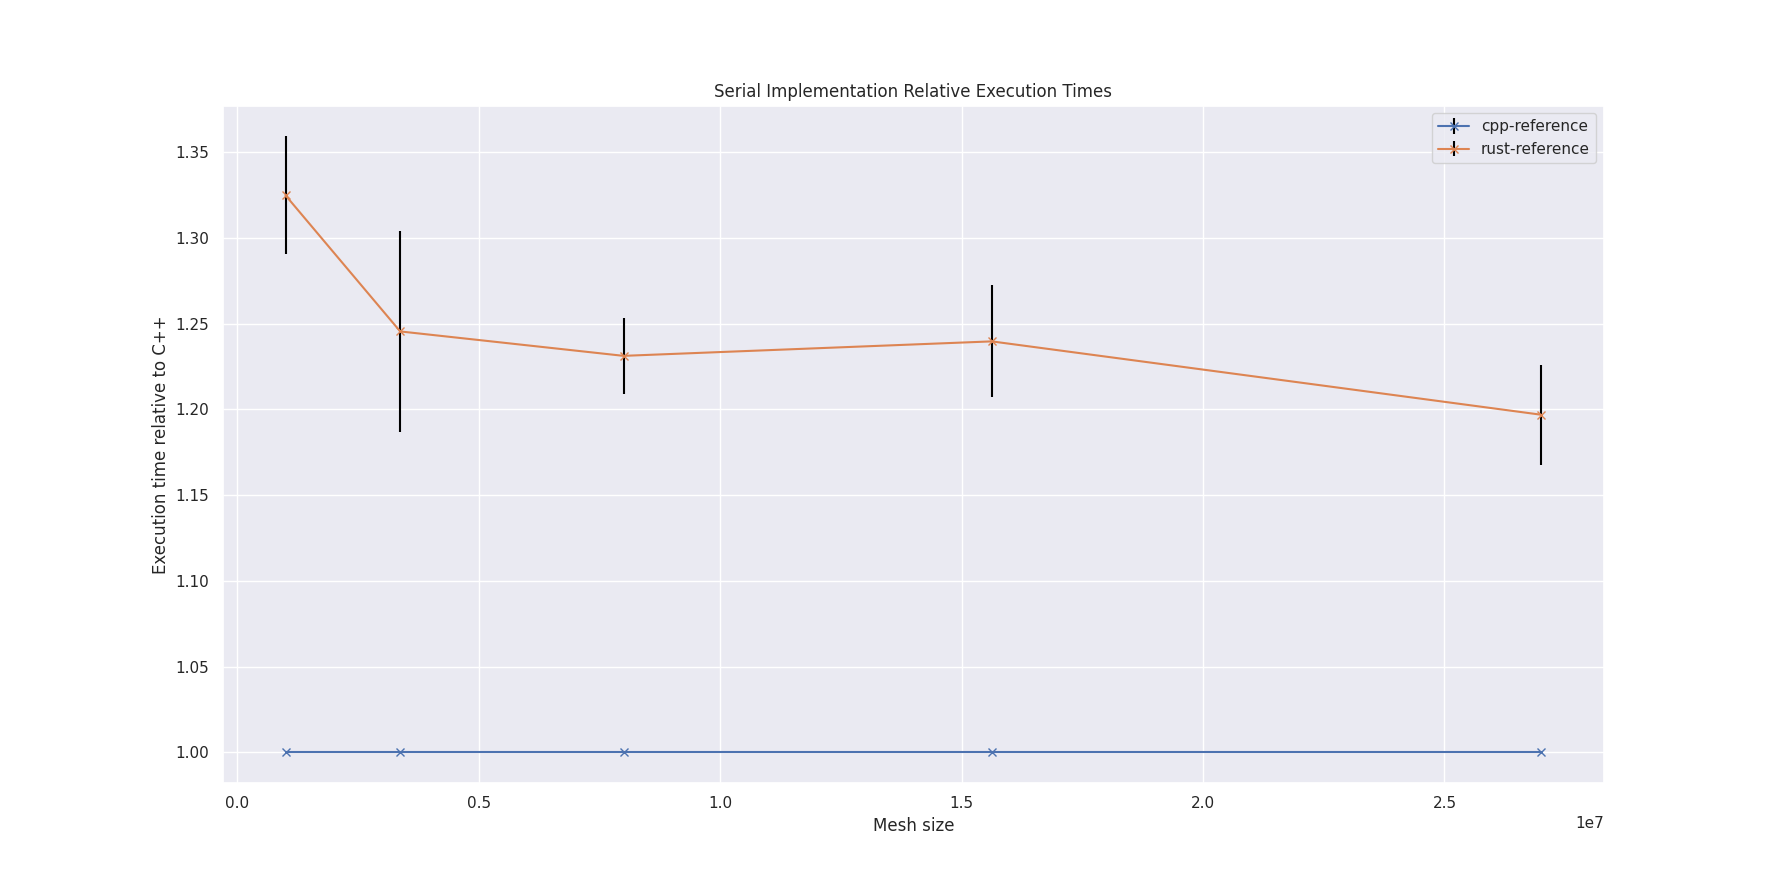
\includegraphics[width=\textwidth]{images/5_performance/parallelism/2_serial_line_relative_avon.png}
    \caption{A line plot comparing the total wall times relative to the C++ implementation of HPCCG, on the Avon batch compute system.}
    \label{fig:2_serial_line_relative_avon}
\end{figure}


In summary, Rust is competitively performant for serial workloads, but trails C++ in performance converging to around a $1.33 \pm .02 \times$ slow down on Kudu and $1.21 \pm 0.03 \times$ slow down on Avon for large mesh sizes.

Finally, we can see that tests run on Avon and Kudu have very similar performance characteristics. This is encouraging, since it suggests that Rust is portable across compute clusters topologies, albeit having only tested on Intel CPUs. As a result of this, for future diagrams, only the runs from Kudu will be shown, unless otherwise stated. The diagrams for Avon runs can be generated using the HPC MultiBench tool from the data provided in the \texttt{hpccg-rs-avon-results} repository, as discussed in section \ref{sssec:parallelism-approaches-reproducibility}.
% NOTE: Or could be shown in Appendix, or just shown inline - this isn't trying to hide anything, its literally just 50 diagrams take a tonne of space...

\subsection{Multi-threading}
\label{ssec:multi-threaded}

Having evaluated serial execution, the next parallelisation strategy to consider is shared memory parallelism through multi-threading. This is typically used for parallelism within a single machine, but it can also be used in combination with MPI for nodes in a cluster, as discussed in section \ref{multi-node-mpi}. As it is such a ubiquitous mechanism of parallelisation, along with frameworks such as OpenMP and Rayon which provide convenient abstractions over it, multi-threading is a critical aspect of writing performant code in High-Performance Computing.

To assess multi-threaded performance, we ran the C++ and Rust executables over both a range of mesh sizes, from $100 \times 100 \times 100$ to $400 \times 400 \times 400$, incrementing each axis size by $50$ each time, and a range of thread counts, from $1$ to $32$, doubling each time. For the parallel tests, all runs were conducted on a single node in the compute cluster, with a single task per node, and 32 threads allocated per task, along with exclusive use of that node to reduce machine noise from other processes. As discussed in the previous section, only runs from the Kudu batch compute system will be shown for brevity, unless the results on Avon notably differ. The results of these experiments are shown in Figures \ref{fig:5_parallel_line_all} and \ref{fig:7_parallel_line_relative}.

\begin{figure}[H]
    \centering
    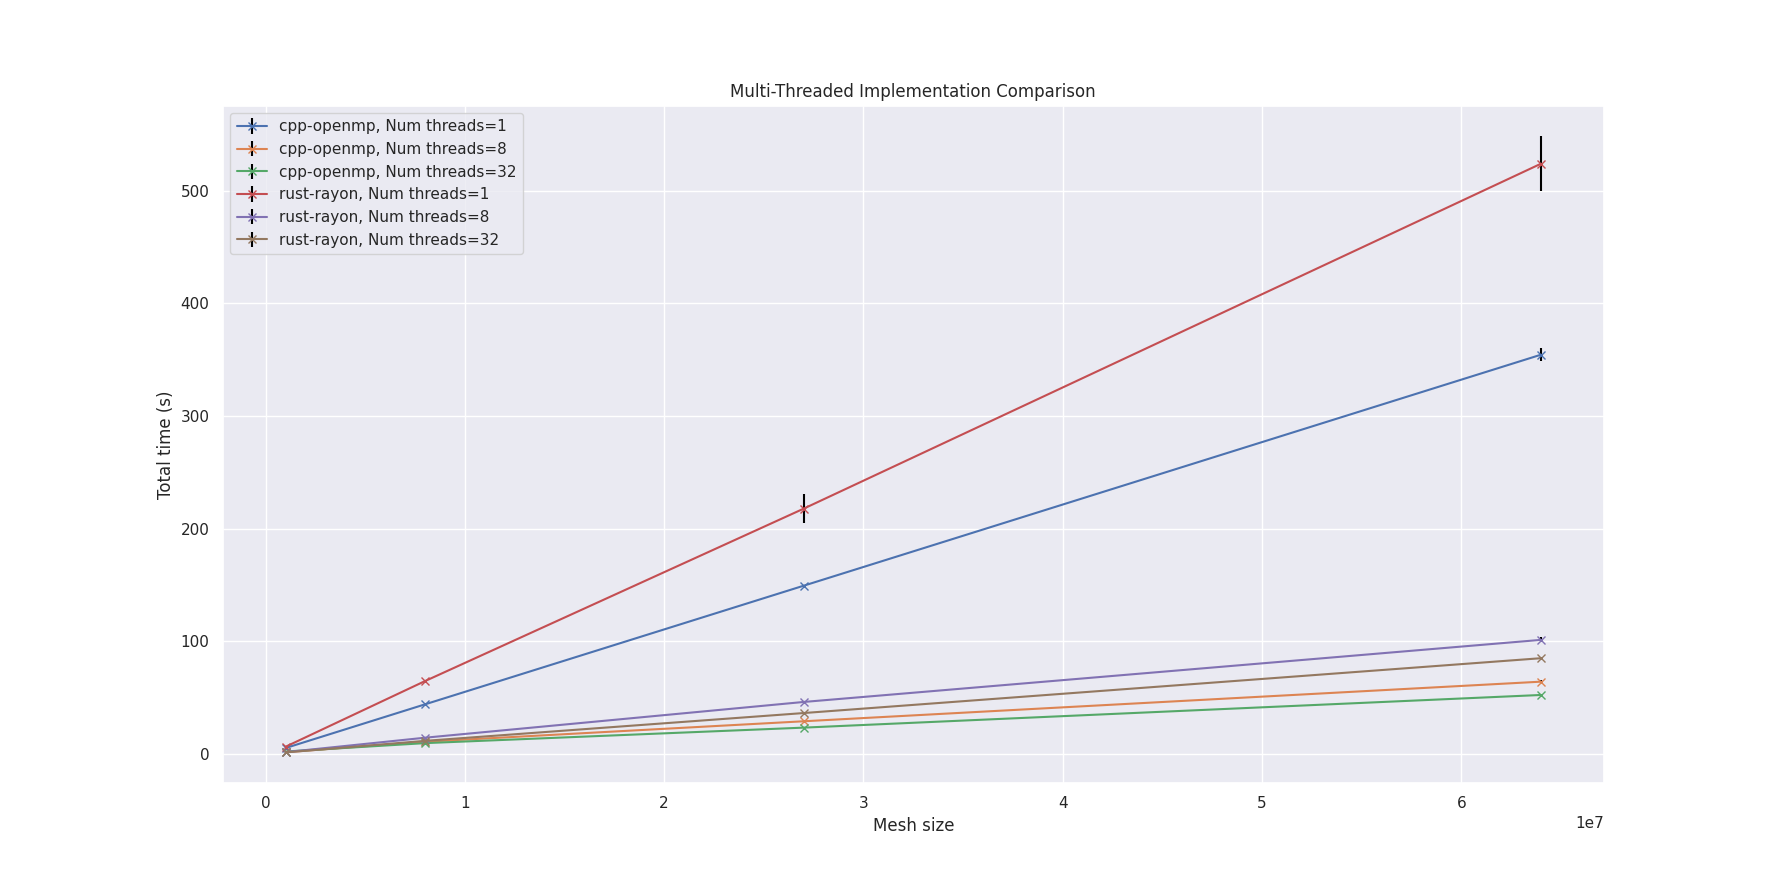
\includegraphics[width=\textwidth]{images/5_performance/parallelism/5_parallel_line_all.png}
    \caption{.}
    \label{fig:5_parallel_line_all}
\end{figure}

\begin{figure}[H]
    \centering
    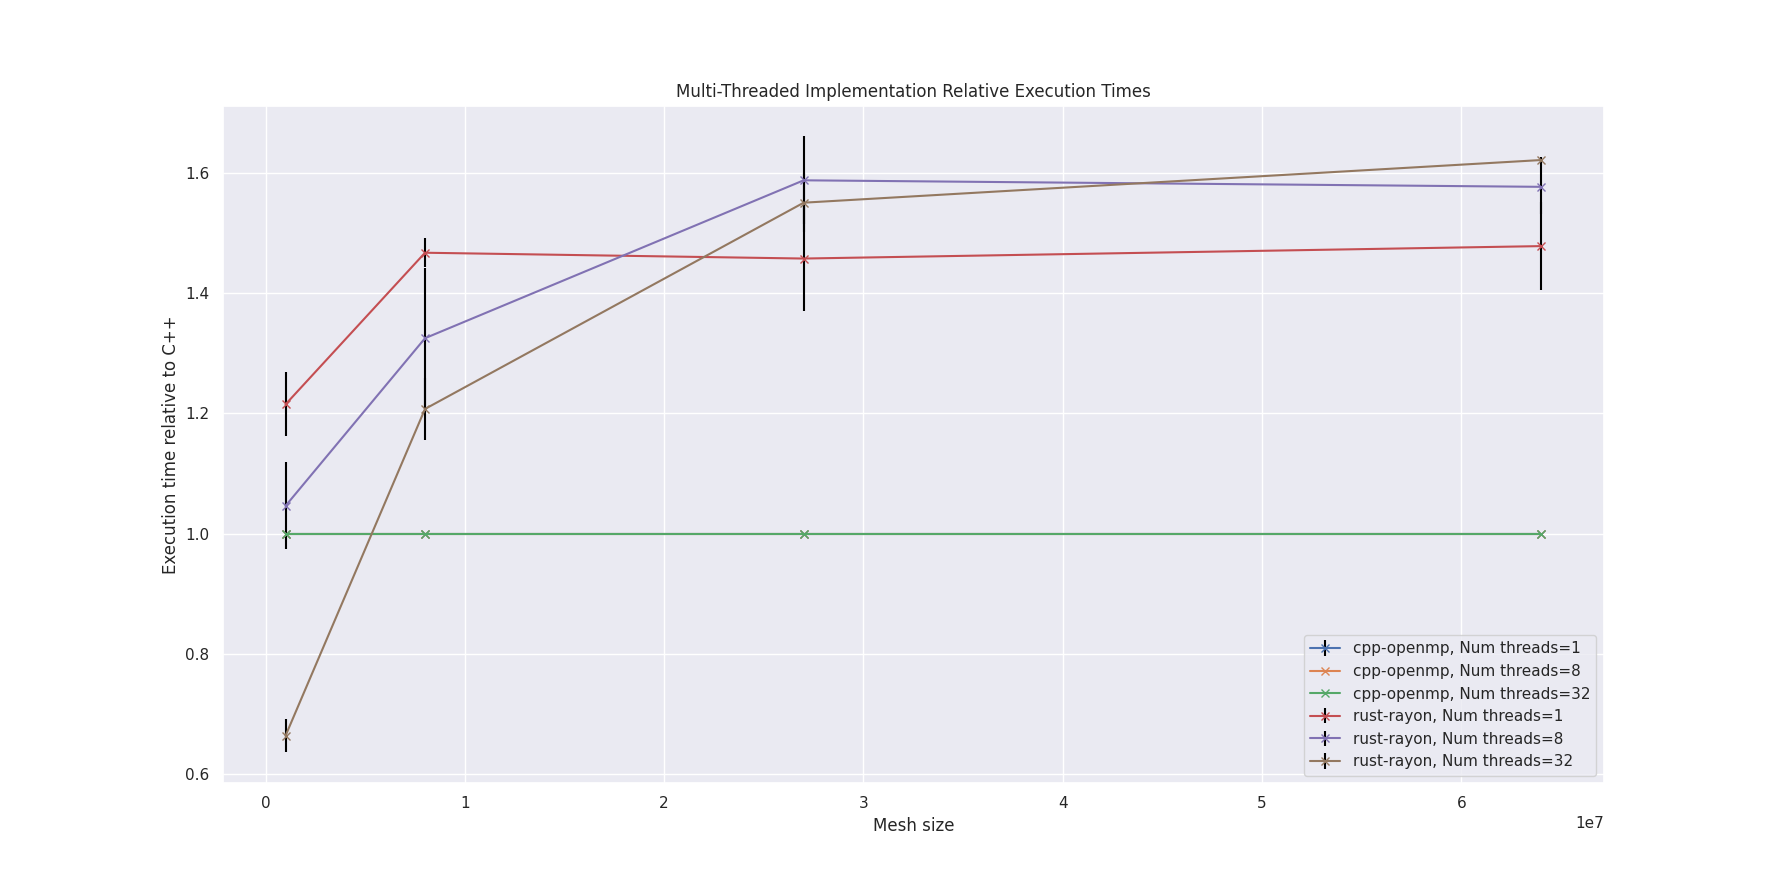
\includegraphics[width=\textwidth]{images/5_performance/parallelism/7_parallel_line_relative.png}
    \caption{.}
    \label{fig:7_parallel_line_relative}
\end{figure}

From Figure \ref{fig:7_parallel_line_relative} which shows execution time relative to C++, we can see that for small meshes Rust with Rayon outperforms C++ with OpenMP increasingly with higher thread counts. For $100 \times 100 \times 100$ meshes with 32 threads, Rust takes $0.66 \pm 0.08 \times$ less runtime. This is likely because Rayon uses a work-stealing thread scheduling methodology, which means it avoids the overhead of allocating many threads for tasks too small to fully leverage them.

However, for the largest workload of $400 \times 400 \times 400$ rusts begins to significantly trail C++, with 32 threads being $1.621 \pm 0.005 \times$ slower. This slower runtime appears to converge for very large mesh sizes, for example with 8 threads, meshes with edge lengths of $300$ and $400$ overlap uncertainty intervals at $1.49 \pm 0.12$ and $1.51 \pm 0.11$ respectively. This convergence appears to occur later for higher thread counts, but further experimentation on a more capable machine would be required to confirm this.

In summary, Rust remains performant in multi-threading workloads, but trails C++ in performance with around a $1.5 \pm 0.1\times$ slow down for large, highly parallel workloads. The results from runs on Avon match those from those shown above on Kudu, with the slowdown across threads similarly converging at around $1.5 \pm 0.25$.

\subsection{MPI}
\label{ssec:mpi}

Shared memory parallelism is a very powerful technique for enhancing program performance. However, its efficacy is upper bounded by being constrained to a single machine with a shared memory architecture. In order to scale beyond this, distributed memory parallelism must be leveraged. This is required for many High-Performance Computing applications, as the largest supercomputers are all composed of clusters of many machines \cite{HomeTOP500}. As discussed in the translation section \ref{}, Rust provides MPI bindings which facilitate this.

To assess performance using MPI for message passing, we ran the C++ and Rust executables over both a range of mesh sizes, from $25 \times 25 \times 25$ to $250 \times 250 \times 250$, incrementing each axis size first by $25$, then by $50$ each time, and a range of nodes $1$, $2$, and $4$, with one task per node. For the MPI implementation, mesh size is constrained by the reference implementation constant value \mintinline{c++}{const int max_external = 100000;}. As a result of this, experiments ran only up to $250 \times 250 \times 250$ rather than $400 \times 400 \times 400$ for parallel implementations. Future work could include increasing this value and fixing any associated bugs, then running HPCCG across many nodes on a much larger mesh. 
% TODO: large run with this turned up, then reference it here.
The results of these experiments are shown in Figures \ref{fig:9_mpi_line} and \ref{fig:10_mpi_line_relative}.

\begin{figure}[H]
    \centering
    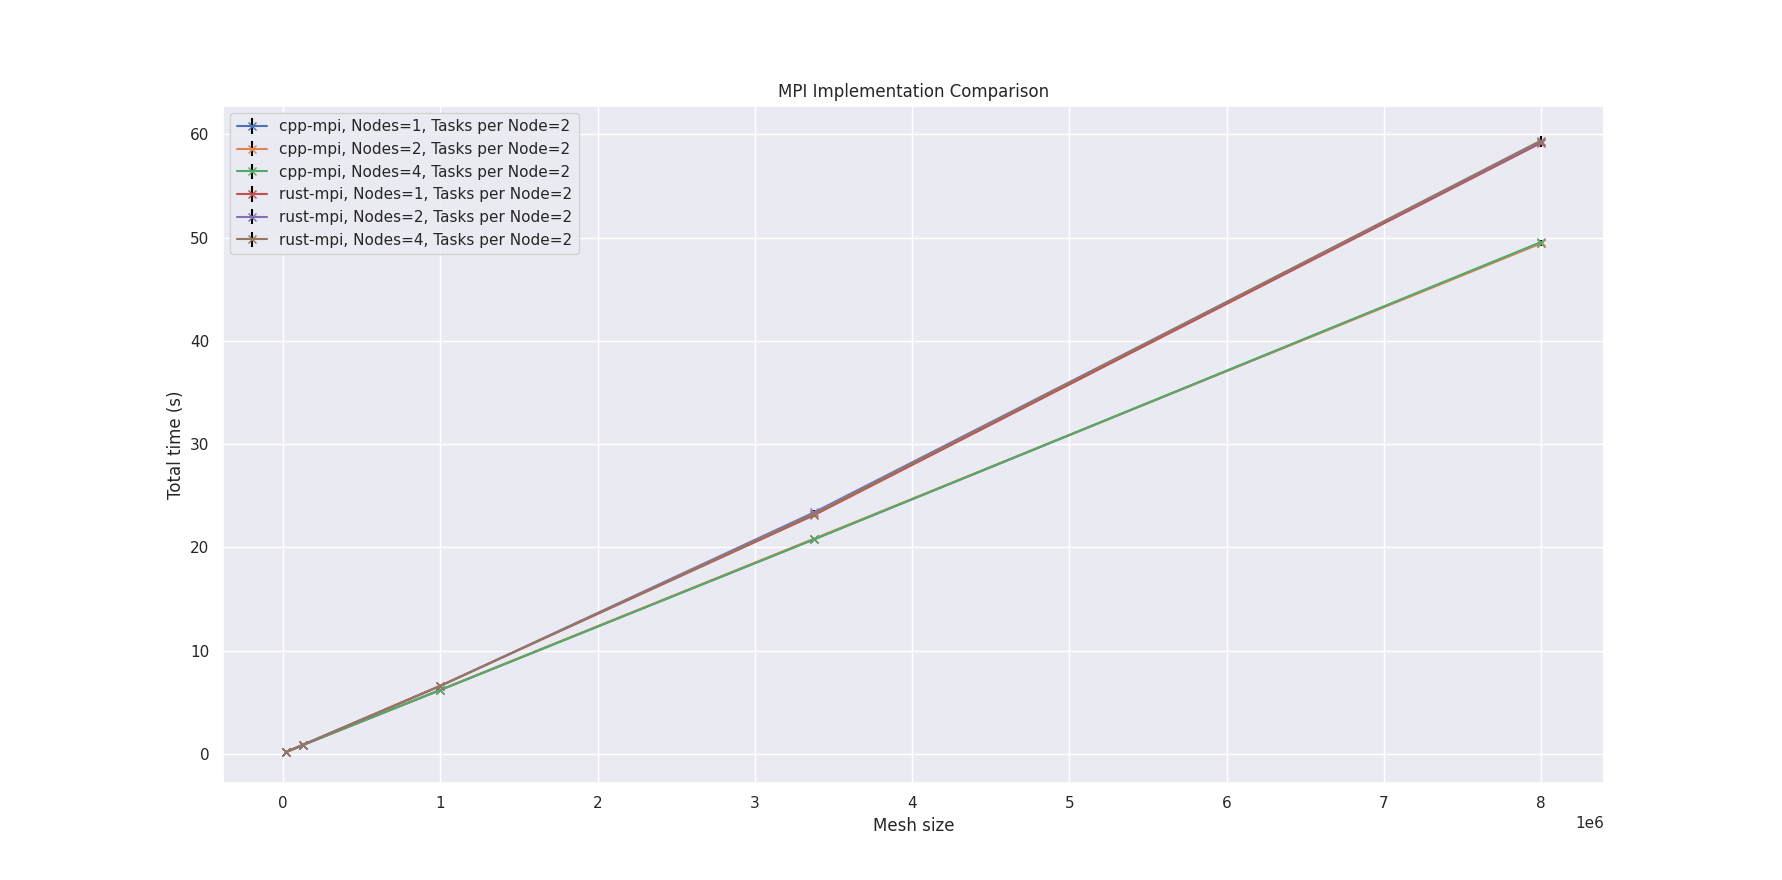
\includegraphics[width=\textwidth]{images/5_performance/parallelism/9_mpi_line.png}
    \caption{.}
    \label{fig:9_mpi_line}
\end{figure}

\begin{figure}[H]
    \centering
    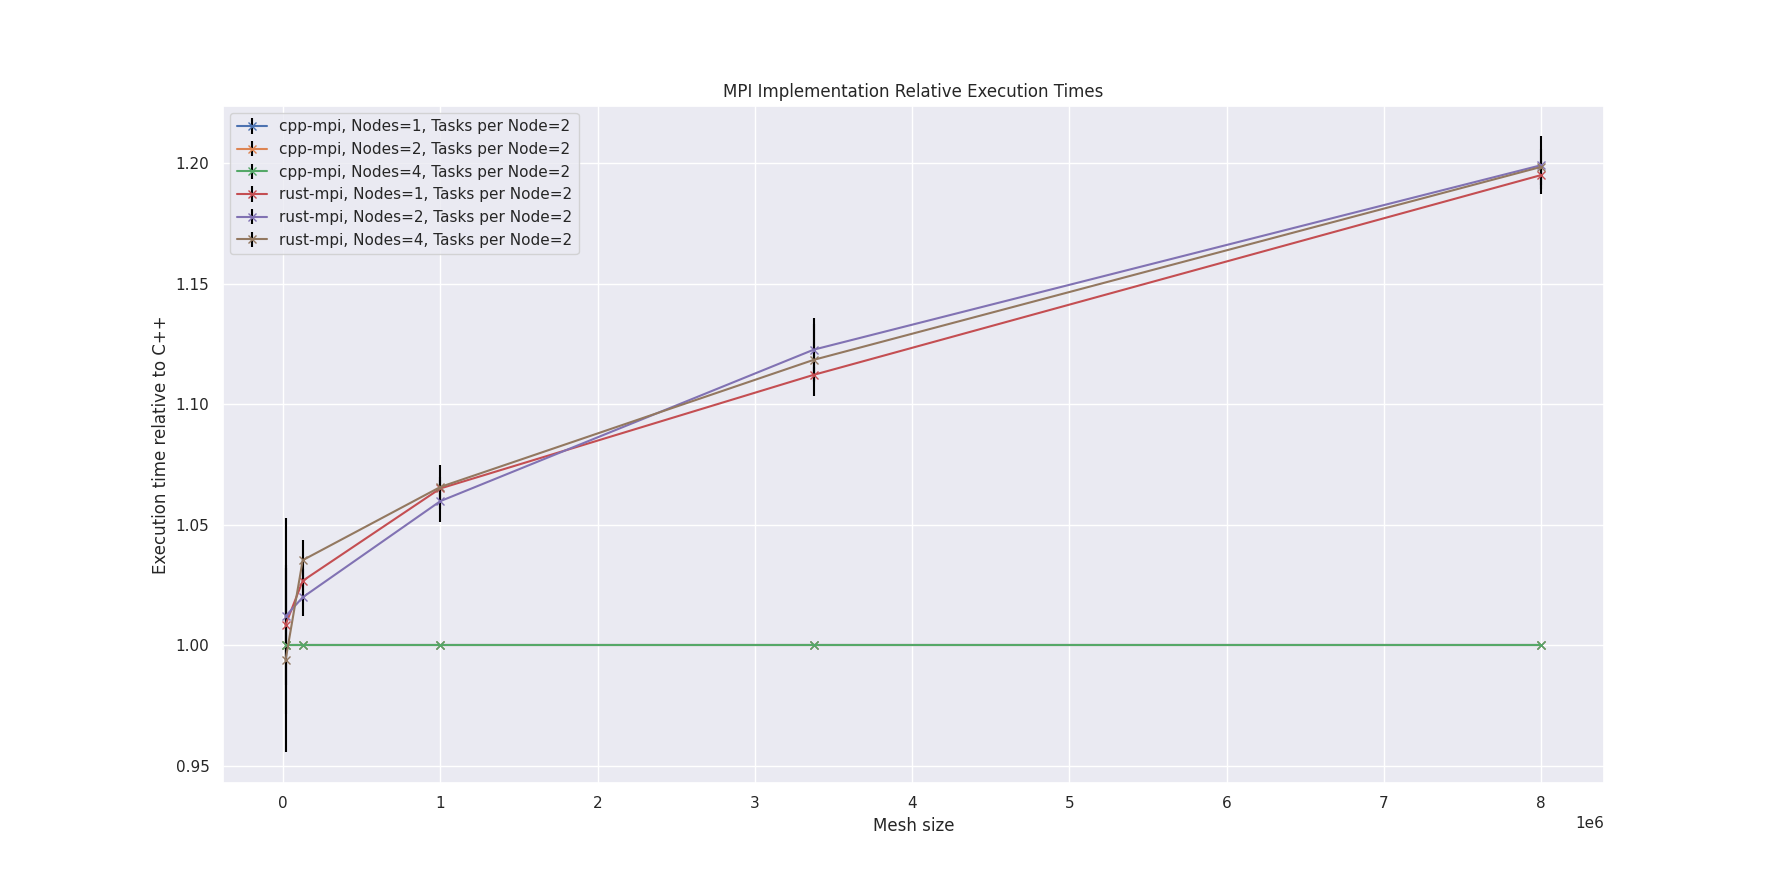
\includegraphics[width=\textwidth]{images/5_performance/parallelism/10_mpi_line_relative.png}
    \caption{.}
    \label{fig:10_mpi_line_relative}
\end{figure}

% TODO: Consider re-running this test, could be a misconfiguration in the YAML dispatching (discuss in the paragraph)
% NOTE: Looks like Slurm is dispatching all runs to four nodes? Investigate and change metrics?
In Figure \ref{fig:9_mpi_line}, we can see that the performance trends form two tight bundles, one of the C++ implementations and one of the Rust implementations. All data points in these bundles are within each others uncertainty intervals, suggesting that there is no increase in performance as a result of adding more MPI tasks for this workload. Since this property is shared by the implementation in both languages, this indicates overhead introduced in communication latency by adding nodes is approximately equal to the performance gain by increasing the number of tasks concurrently processing the data. However, this property is still desirable, as it allows very large mesh sizes to be scaled across clustered compute resources, which can then leverage multi-threading within each machine, as discussed in the next section.

Alternatively, this result could be an unexpected emergent property of dispatching many Slurm jobs, which might over-allocate the number of nodes to be the maximum across all jobs, hence resulting in no change across the intended degrees of parallelism.

This is measured property is further confirmed by Figure \ref{fig:10_mpi_line_relative} showing the relative performance, again with tightly bundled trends for Rust and C++. The decrease in relative performance of Rust appears to be trending up without converging within the range of this experiment. Ideally, the mesh size would be increased till this decrease converged to a value, but the previously discussed structural limitations of the HPCCG mini-app prevent such runs being measured.

In summary, Rust remains performant in message passing workloads, but trails C++ in performance with around a $1.19 \pm 0.01\times$ slow down, with the expectation this will converge to a higher value for larger workloads, likely to around the serial slow down of $1.5 \pm 0.1\times$, as both implementations invoke the same implementation of MPI. The results from runs on Avon match those from those shown above on Kudu, with the slowdown across threads similarly converging at around $1.5 \pm 0.25$.

% \subsection{MPI with Multi-threading}
% \label{ssec:mpi-multithreading}

% Shared and distributed memory parallelism can be used in tandem, with multi-threading within machines, which then communicate with each other through message passing. This allows programmers to leverage desirable properties from both approaches, such as the low-overhead performance of multi-threading in combination with the scalability of message passing.

% This assessment shows a compares a best-case scenario for MPI with Multi-threading, which best characterises a likely use case in High-Performance Computing. Four nodes are used, with one task per node, and 32 threads per task. As such, four MPI ranks are used in combination with 32 threads for a total parallelism degree of 128 concurrent execution paths. This configuration was then driven over the same test range as MPI, from $25 \times 25 \times 25$ to $250 \times 250 \times 250$, incrementing each axis size first by $25$, then by $50$ each time. This is again constrained by the \texttt{max\_external} constant in the reference implementation. The results of these experiments are shown in Figures \ref{fig:12_hybrid_line} and \ref{fig:13_hybrid_line_relative}.

% \begin{figure}[H]
%     \centering
%     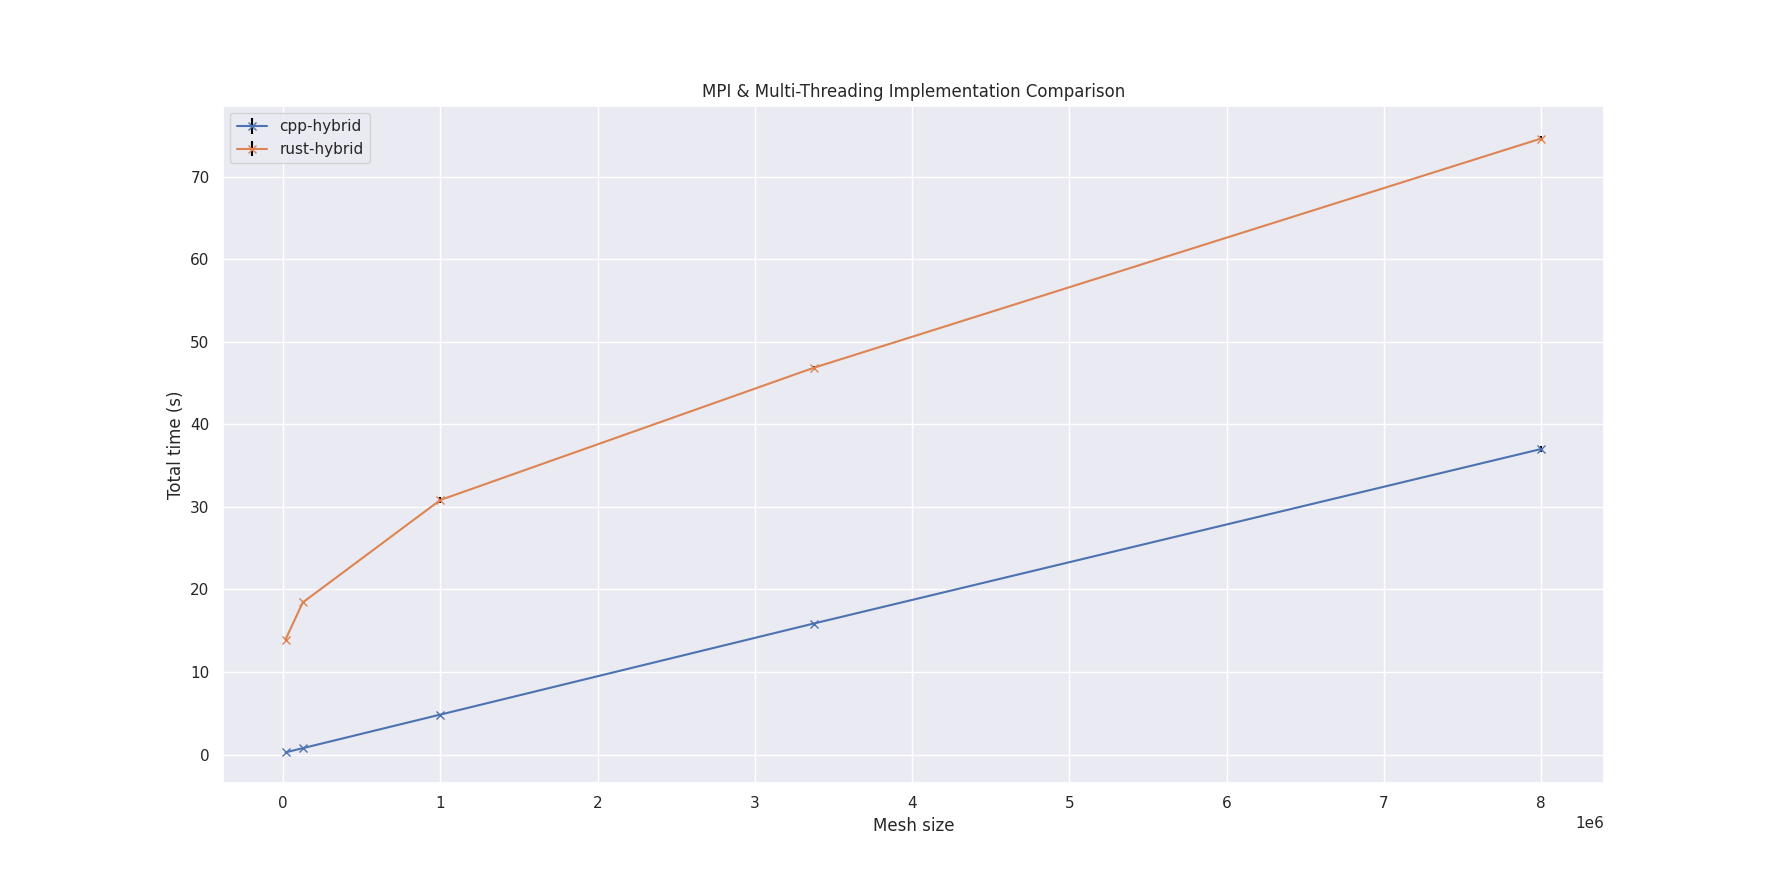
\includegraphics[width=\textwidth]{images/5_performance/parallelism/12_hybrid_line.png}
%     \caption{.}
%     \label{fig:12_hybrid_line}
% \end{figure}

% \begin{figure}[H]
%     \centering
%     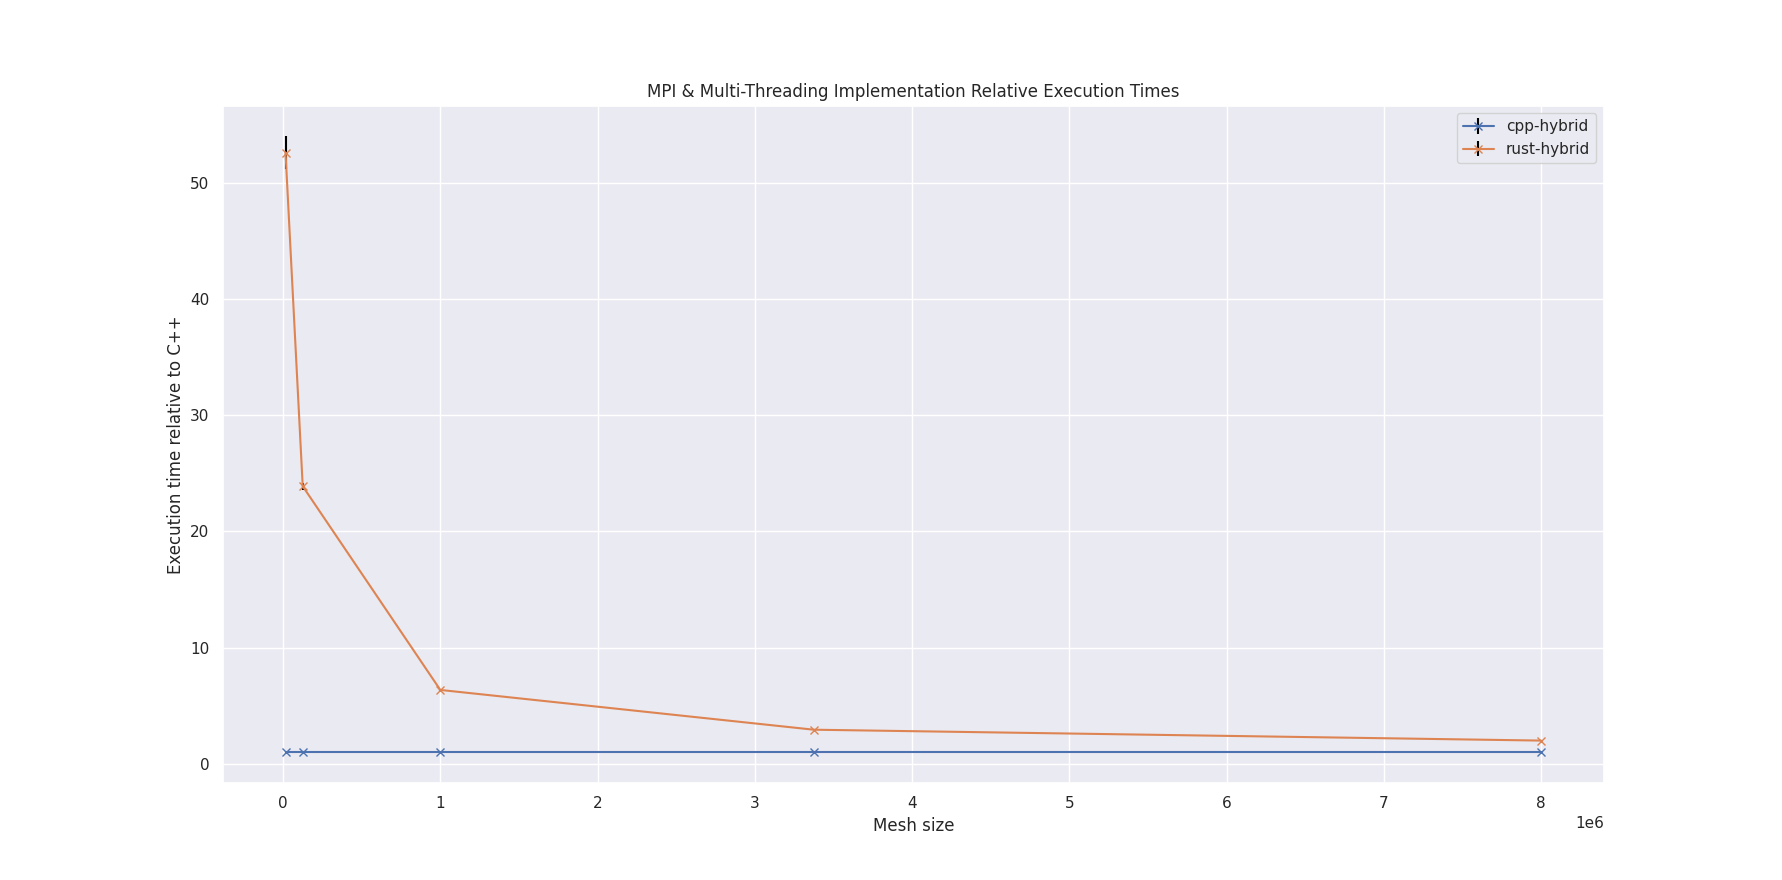
\includegraphics[width=\textwidth]{images/5_performance/parallelism/13_hybrid_line_relative.png}
%     \caption{.}
%     \label{fig:13_hybrid_line_relative}
% \end{figure}

% % Analysis

% In summary,


\subsection{Performance portability frameworks}
\label{ssec:performance-portability-frameworks}

Finally, performance portability frameworks, such as Kokkos \cite{KokkosEcosystem}, are commonly used within High-Performance Computing to allow writing software which can run across a variety of hardware. However, such frameworks often incur a performance cost over hand-optimised implementations targeted at specific hardware. The fact that these frameworks are common, despite this performance cost, motivates the idea that Rust could be suitable for High-Performance Computing as a result of its productivity benefits, despite its performance impact.

This assessment compares the Rust, Kokkos, and C++ executables performance over a range of mesh sizes, from $25 \times 25 \times 25$ to $400 \times 400 \times 400$, incrementing each axis size first by $25$, then $50$, then $100$ for the remaining increments. As with the parallel assessment, a single node and a single task per node is used, and the implementations are compared with 32 threads each. The results of these experiments are shown in Figures \ref{fig:16_kokkos_line} and \ref{fig:17_kokkos_line_relative}.

\begin{figure}[H]
    \centering
    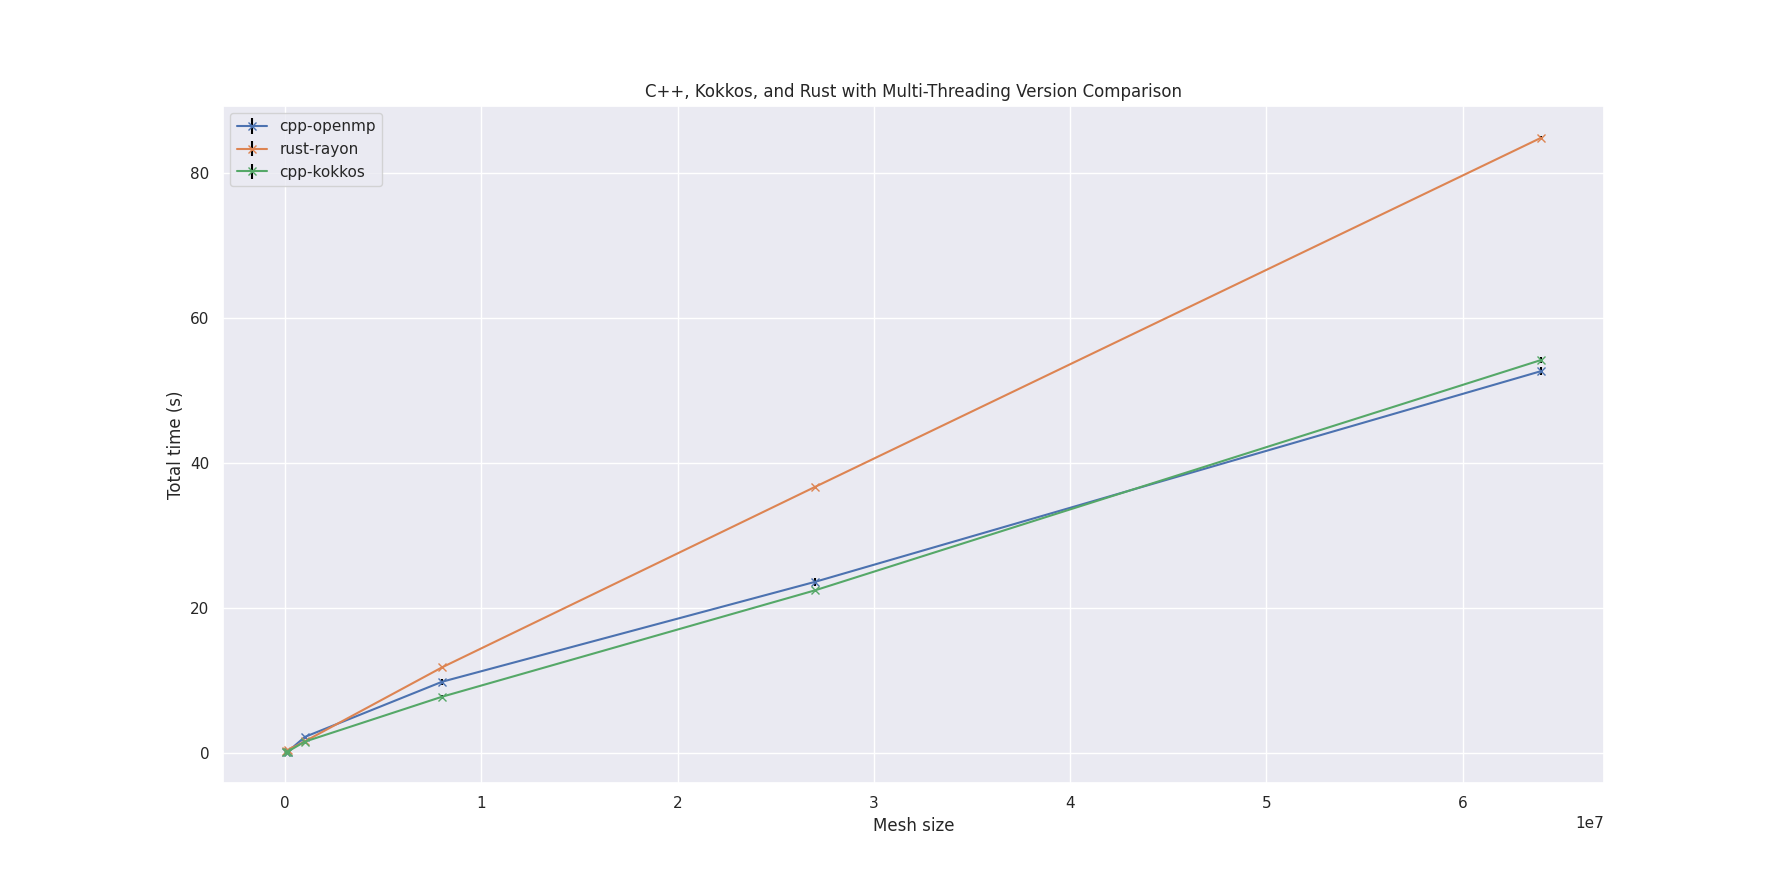
\includegraphics[width=\textwidth]{images/5_performance/parallelism/16_kokkos_line.png}
    \caption{.}
    \label{fig:16_kokkos_line}
\end{figure}

\begin{figure}[H]
    \centering
    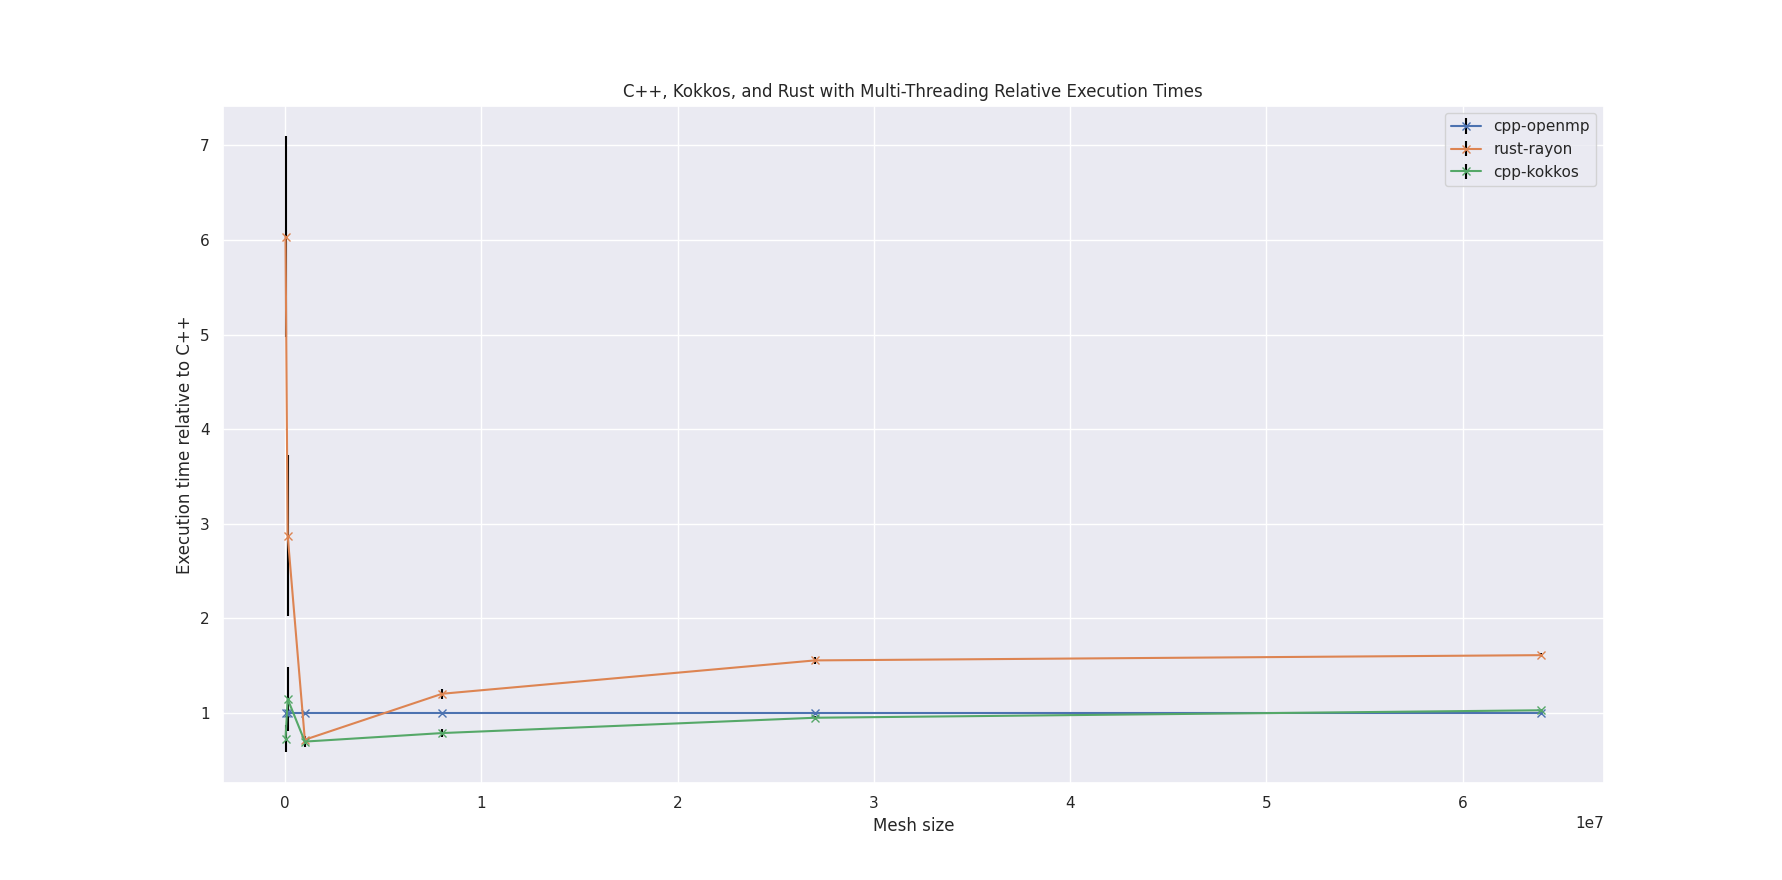
\includegraphics[width=\textwidth]{images/5_performance/parallelism/17_kokkos_line_relative.png}
    \caption{.}
    \label{fig:17_kokkos_line_relative}
\end{figure}


From Figure \ref{fig:16_kokkos_line} which shows execution time of the Rust and Kokkos implementations, relative to C++. Here, we can see that Kokkos out-performs C++ for small mesh sizes, but as the mesh size grows begins to incur a performance cost beyond C++. From \ref{fig:17_kokkos_line_relative} we can quantitatively see that for the largest $400 \times 400 \times 400$ mesh, the Kokkos implementation has a $1.03 \pm 0.01 \times$ slow down, and the Rust implementation has a $1.61 \pm 0.02 \times$ slow down. 

In this set of results, the slow down of Kokkos is not sufficiently comparable to that of Rust to motivate the performance-productivity trade-off. However, the benchmarked implementation uses Kokkos for parallelism only, without modifying the data structure, so may underreport the upper bound for the performance impact of Kokkos. % TODO: Find a paper with this upper bound


% \section{Summary of results}
% \label{sec:performance-results}

% Performance

% Productivity
\chapter{Project Management}
\label{ch:project-management}

% https://warwick.ac.uk/fac/sci/dcs/teaching/material/cs310/components/final/marking/management
% Organisation: Did the student plan their activities in advance and keep to the plan? Did the student exhibit good time-management skills?
% Specification: Did the student make clear at the start of the project what they intended to do?
% Effort and motivation: Did the student work hard?
% Professionalism: Has the student taken into account matters such as ethics, social issues, and the law, as they relate to the project?


\section{Legal, social, ethical and professional issues}
\label{sec:legal-social-ethical-professional-issues}
% TODO: Decide on sentence vs title case and be consistent throughout

\chapter{Conclusions}
\label{ch:conclusions} % 500 words intro

% The project is a success. Summarise what you have done and accomplished.


\section{Reflection}
\label{sec:reflection} % 800 words

\section{Open source work}
\label{sec:open-source-work} % 500 words

% UK-MAC PR for website
% autocxx unit tests PR

\section{Future work}
\label{sec:future-work} % 250 words

% Suggest what projects might follow up on this. The suggestions here should \textbf{not} be small improvements to what you have done, but more substantial work that can now be done thanks to the work you have done or research questions that have resulted from your work.



%TC:ignore
\bibliographystyle{IEEEtran}
\bibliography{bibliography}

\appendix

\chapter{Project collateral}
\label{ch:project-collateral}

\section{Project Requirements}
\label{sec:project-requirements}

The specification document enumerated the set of MoSCoW prioritised \cite{CaseMethodFastTrack} requirements which unambiguously define the project scope. These requirements are replicated below:

\begin{enumerate}
\item
  Select a target mini-app from ECP proxy applications or UK-MAC
  (\textbf{Must have})
\item
  Fuzz test\footnote{an automated testing technique which uses boundary and erroneous test data as inputs, whilst monitoring for resultant undesired behaviour, originally proposed by Miller \textit{et al.} in 1990 \cite{millerEmpiricalStudyReliability1990}\cite{liangFuzzingStateArt2018}} the possible mini-apps for memory safety issues using static analysis tooling \cite{stepanovMemorySanitizerFastDetector2015}
  (\textbf{Should have}, \textit{depends on 1})
\item
  Build tooling for running Rust unit tests on C++ code
  (\textbf{Could have})
\item
  Write unit tests for the original C++ version of the
  mini-app
  (\textbf{Should have}, \textit{depends on 1, (3)})
\item
  Write direct translation of serial version mini-app from C++ to Rust
  (\textbf{Must have}, \textit{depends on 1})
\item
  Modify serial version of translated code to be idiomatic Rust \cite{endlerMreIdiomaticrust2023} 
  (\textbf{Should have}, \textit{depends on 5})
\item
  Equivalence check serial translated code by comparing results of end-to-end tests with original C++ code
  (\textbf{Must have}, \textit{depends on 5}))
\item
  Equivalence check serial translated code by applying passing C++ unit tests to rust code
  (\textbf{Must have}, \textit{depends on 4, 5})
\item
  Equivalence check serial translated code with limited formal verification techniques
  (\textbf{Could have}, \textit{depends on 5})
\item
  Equivalence check serial translated code by comparing generated LLVM IR of the C++ and translated Rust versions
  (\textbf{Could have}, \textit{depends on 5})
\item
  Modify the serial translated code to allow parallel execution
  (\textbf{Must have}, \textit{depends on 5})
\item
  Equivalence check parallel translated code via all previous techniques
  (\textbf{Must have}, \textit{depends on 7, 8, (9), (10), 11})
\item
  Carry out a performance analysis of the serial translated Rust code with the original C++ code
  (\textbf{Must have}, \textit{depends on 5})
\item
  Carry out a performance analysis of the parallel translated Rust code with the original C++ code
  (\textbf{Must have}, \textit{depends on 11})
\item
  Modify the parallel translated code to allow execution across clustered compute resources
  (\textbf{Could have}, \textit{depends on 11})
\item
  Equivalence check clustered translated code via all previous techniques
  (\textbf{Could have}, \textit{depends on 7, 8, (9), (10), 15})
\item
  Carry out a performance analysis of the clustered translated Rust code with the original C++ code
  (\textbf{Could have}, \textit{depends on 15})
\end{enumerate}

\section{Mini-app selection}
\label{sec:miniapp-selection}



\section{Mini-app selection process}
\label{sec:miniapp-selection}

A significant component of early project planning was selecting the mini-app to perform the translation on. Since the translation process would take a significant amount of time, and could be heavily impacted by the properties of the chosen mini-app, it was vital to make an informed selection. The selection process for the mini-app is described below, broadly replicated from the progress report document:

The first objective set out in the specification was ``Select a target mini-app from ECP proxy applications or UK-MAC (\textbf{Must have})'', and all other objectives trivially have a dependency on it.

% Criteria for selection
Between the ECP Proxy Applications \cite{ECPProxyApplications} and UK-MAC \cite{UKMiniAppConsortium}, there were 91 possibilities from which to narrow down. The criteria for initial filtering of the mini-apps was:
\begin{itemize}
    \item The source code for the mini-app must be C++ only (no FORTRAN or Python), in order to conform to the project specification.
    \item The mini-app must not use any High-Performance Computing frameworks, such as Kokkos \cite{KokkosEcosystem} or RAJA \cite{RAJAPortabilitySuite}. This is because they may not have Rust bindings, and the translation of a whole performance framework it out of scope for the project.
    \item The source code for the mini-app must be available as a repository on GitHub, as access to the source code is necessary for the translation process.
\end{itemize}

% Script built for selection
Due to the number of possible applications, a script was written to filter the applications by these criteria. First, the script makes a web request to the page for the application, for example \href{https://proxyapps.exascaleproject.org/app/minimd/}{miniMD}, and parses the unstructured HTML data from this website into a Polars DataFrame \cite{PolarsPolars2023}. If the application has a link to a GitHub repository, it also includes data from a request to the GitHub API \cite{GitHubRESTAPI}. Finally, it uses the scraped data to deselect mini-apps if they don't meet the criteria.

\begin{figure}[h]
    \centering
    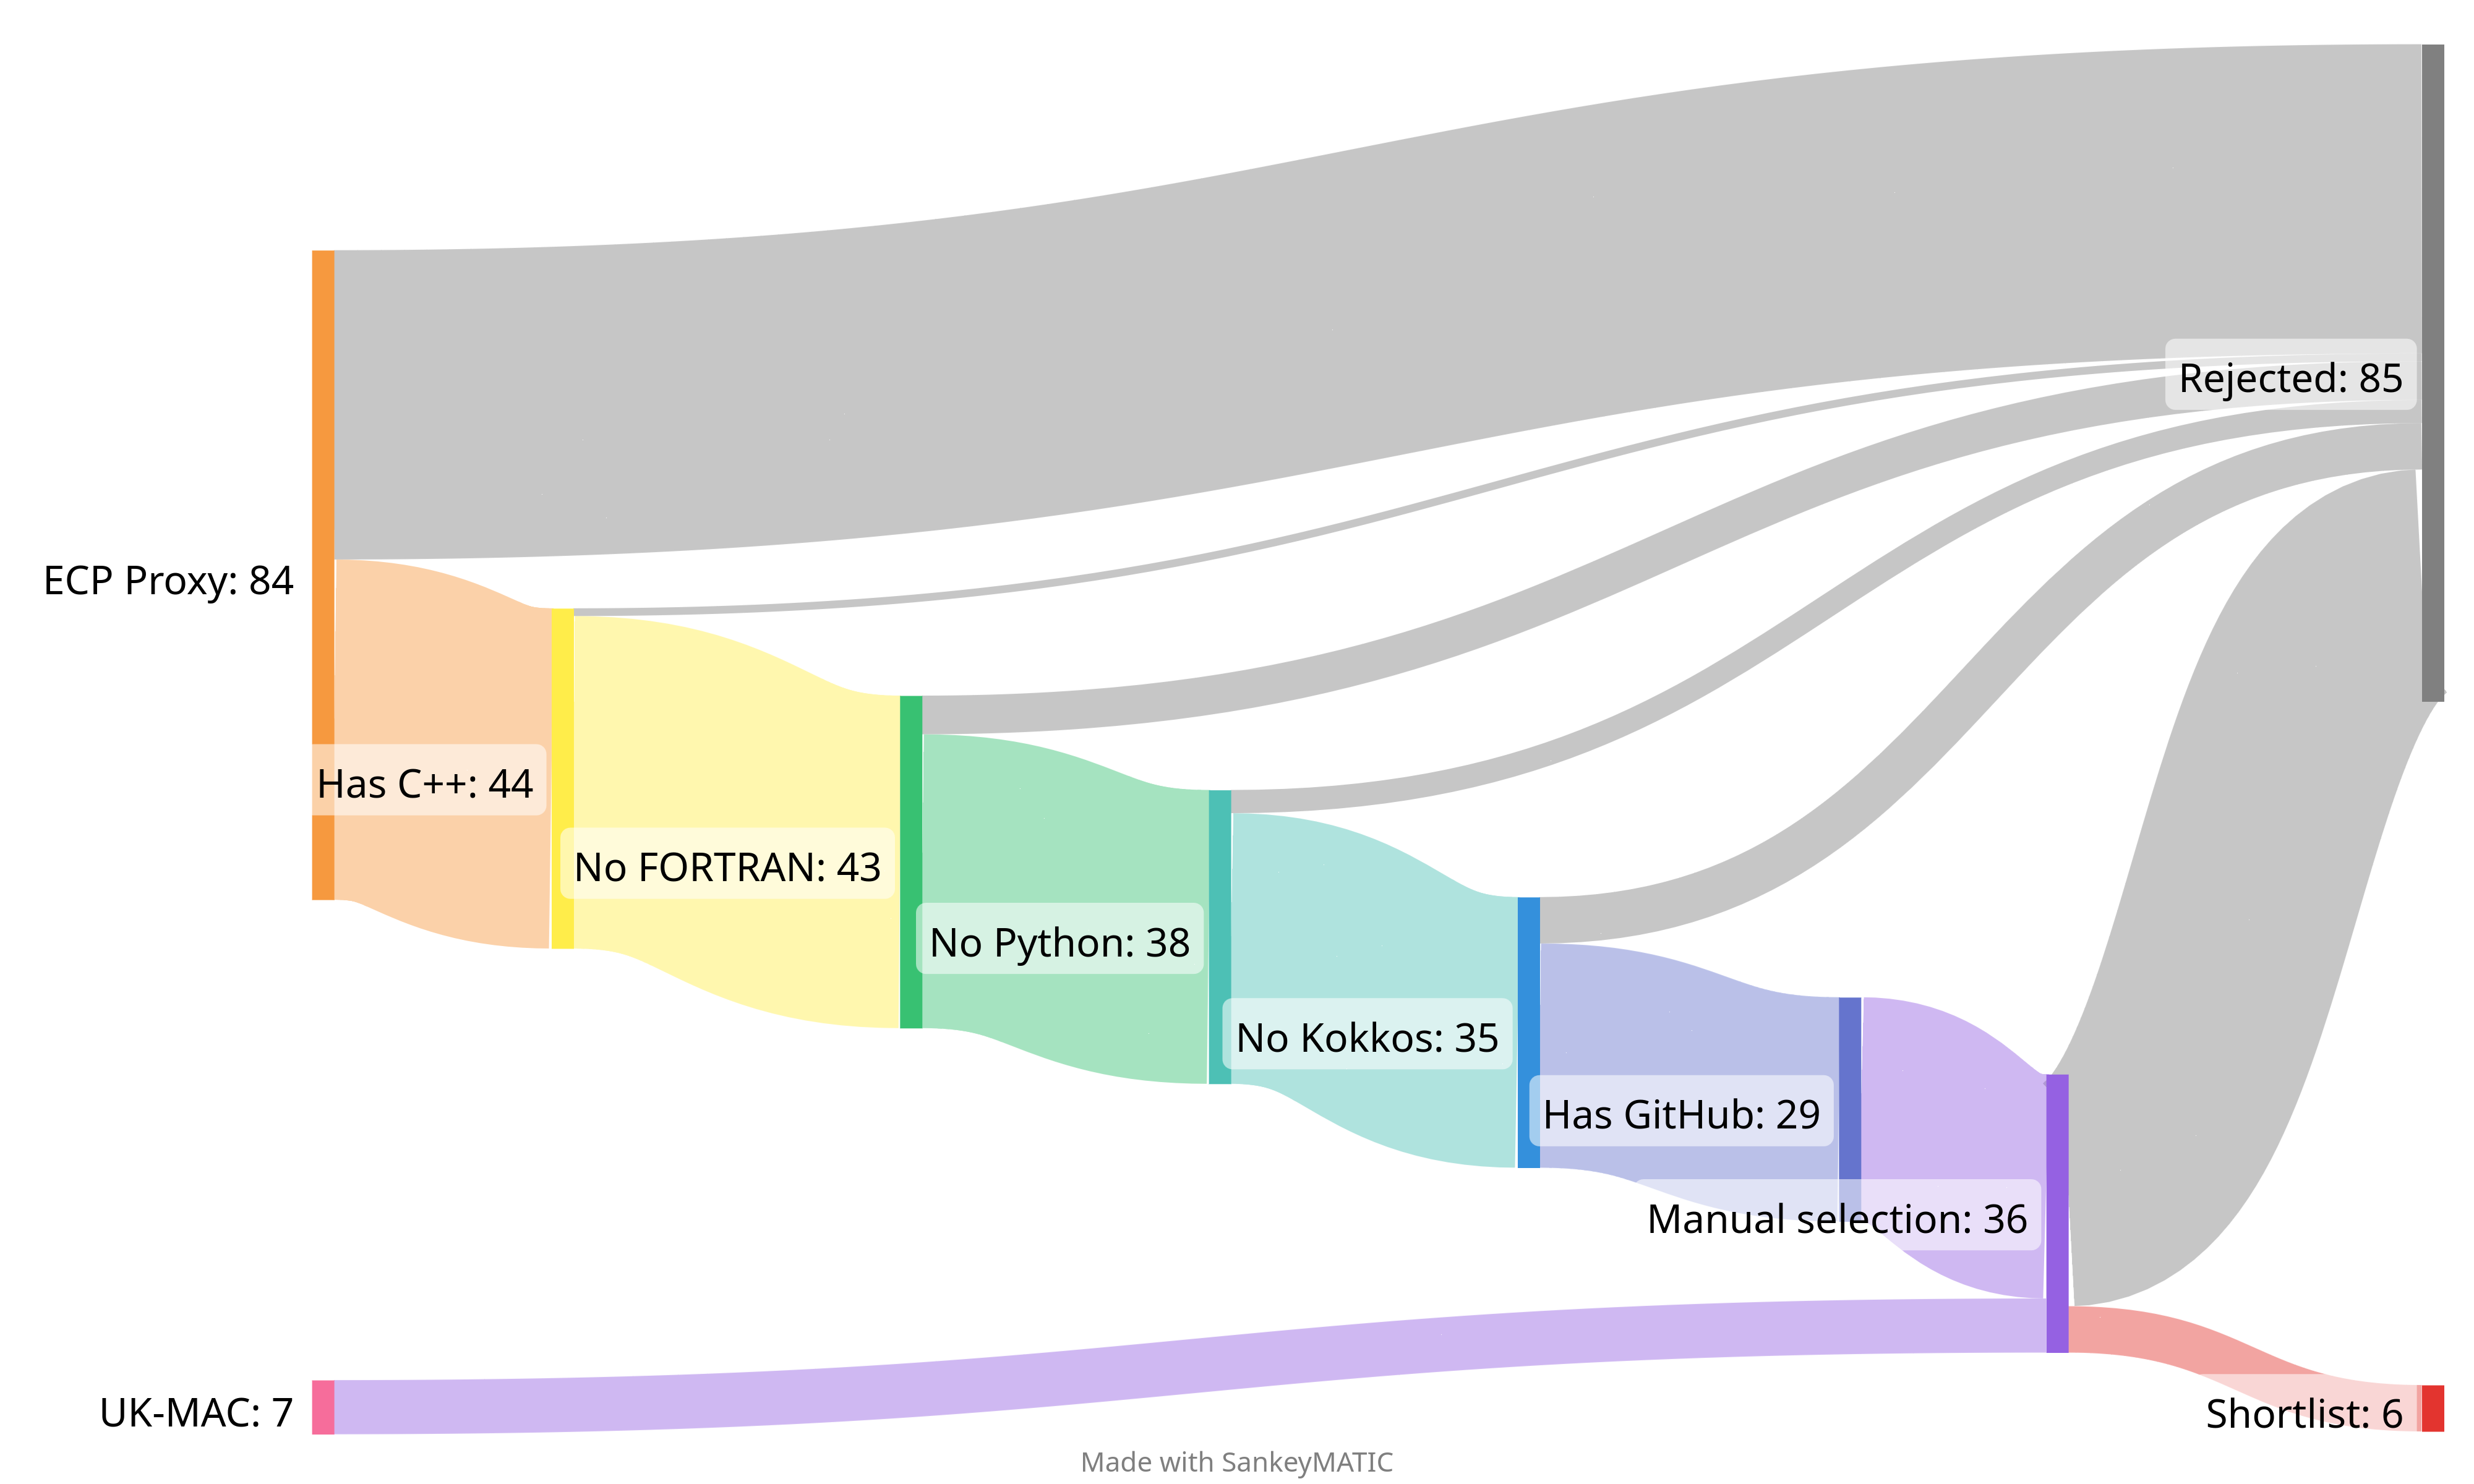
\includegraphics[width=0.75\textwidth]{images/8_appendix/miniapp_sankey.png}
    \caption{A Sankey Diagram showing the selection process for the mini-apps, generated by \href{https://sankeymatic.com/build/}{SankeyMatic}.}
    \label{fig:miniapp_sankey}
\end{figure}

After the automated step of the selection process, six of the remaining thirty-six mini-apps were shortlisted, following a discussion with the project supervisor. These shortlisted mini-apps were then manually inspected for the criteria shown in Table \ref{table:miniapps}:

\begin{table}[H]
\centering
    \caption{A table showing the shortlisted mini-apps and their aspects considered when making the final selection.}
    \label{table:miniapps}
    \begin{tabular}{|p{0.14\linewidth}|p{0.125\linewidth}|p{0.12\linewidth}|p{0.1025\linewidth}|p{0.135\linewidth}|p{0.1\linewidth}|}
    \hline
    Name       & Codebase size (lines of code) & Additional dependencies & Tests               & Implemen-tation versions & Memory leaks \\ \hline\hline
    CabanaPIC \cite{ECPcopaCabanaPIC2023} & \cellcolor{green!25}1792 & \cellcolor{red!25}Kokkos & \cellcolor{green!25}Unit and end-to-end & \cellcolor{orange!25}Kokkos only & \cellcolor{red!25}Untested     \\ \hline
    CloverLeaf \cite{CloverLeaf} & \cellcolor{red!25}8045 & \cellcolor{green!25}None & \cellcolor{orange!25}End-to-end & \cellcolor{green!25}Many & \cellcolor{orange!25}None         \\ \hline
    HPCCG \cite{herouxHPCCGSolverPackage2007} & \cellcolor{green!25}1542 & \cellcolor{green!25}None & \cellcolor{orange!25}End-to-end & \cellcolor{orange!25}OpenMP and MPI only & \cellcolor{green!25}375 kB       \\ \hline
    MiniMD \cite{osti_1231191} & \cellcolor{orange!25}4082 & \cellcolor{green!25}None & \cellcolor{orange!25}End-to-end & \cellcolor{green!25}Many & \cellcolor{green!25}5.82 MB      \\ \hline
    TeaLeaf \cite{TeaLeaf2023} & \cellcolor{orange!25}2580 & \cellcolor{green!25}None & \cellcolor{orange!25}End-to-end & \cellcolor{green!25}Many & \cellcolor{orange!25}None         \\ \hline
    VPFFT++ \cite{VPFFT2023}   & \cellcolor{orange!25}3384 & \cellcolor{red!25}Eigen, FFTW & \cellcolor{orange!25}Unit & \cellcolor{orange!25}MPI only & \cellcolor{red!25}Untested     \\ \hline
    \end{tabular}
\end{table}

These mini-apps were manually inspected for the size and quality of their codebase (smaller and higher quality is better, assessed using the \texttt{sloccount} \cite{SLOCCount} and the \texttt{clang-tidy} linter \cite{ClangTidyExtraClang}), whether they had unit tests, whether they had multiple versions for serial/parallel, historical prominence, and whether they had any memory leaks using \texttt{valgrind} \cite{ValgrindHome}.

\begin{figure}[H]
\begin{verbatim}
==33790== 
==33790== HEAP SUMMARY:
==33790==     in use at exit: 5,875,096 bytes in 10 blocks
==33790==   total heap usage: 149 allocs, 139 frees, 6,348,737 bytes allocated
==33790== 
[snip]
==33790== 
==33790== LEAK SUMMARY:
==33790==    definitely lost: 375,096 bytes in 4 blocks
==33790==    indirectly lost: 5,500,000 bytes in 6 blocks
==33790==      possibly lost: 0 bytes in 0 blocks
==33790==    still reachable: 0 bytes in 0 blocks
==33790==         suppressed: 0 bytes in 0 blocks
==33790== 
==33790== For lists of detected and suppressed errors, rerun with: -s
==33790== ERROR SUMMARY: 4 errors from 4 contexts (suppressed: 0 from 0)
\end{verbatim}
    \caption{A snippet of the output of running \texttt{valgrind} on the HPCCG mini-app, with over 375kB directly lost over a test run with mesh size $25 \times 25 \times 25$.}
    \label{fig:minimdValgrindOutput}
\end{figure}

Interestingly, some shortlisted mini-apps, including HPCCG, MiniMD, and TeaLeaf, leak memory -- as shown in the Figure \ref{fig:minimdValgrindOutput}. This is emblematic of one of the main drawbacks of C++ -- the ease with which it is to do manual memory management wrong. In contrast, Rust is designed to abstract away memory management from the programmer, instead focussing on the resultant properties of data ownership and lifetimes.

After a manual comparison process on the aspects shown above, the decision was made to select the HPCCG mini-app for the translation process, due to its: small, high quality codebase and simple build system; absence of additional required dependencies; existing implementations for both OpenMP and MPI; and the presence of memory leaks.





\chapter{HPC MultiBench}
\label{ch:tooling-appendix}

\section{Hardware specifications}
\label{sec:tooling-replication-yaml}

\begin{listing}[H]
%     \begin{minted}[linenos,breaklines]{yaml}
% run_configurations:
%   "cpp-serial":
%     sbatch_config:
%       "nodes": 1
%       "ntasks-per-node": 1
%       "cpus-per-task": 1
%       "exclusive": "mcs"
%       "mem": 60000
%     module_loads: []
%     environment_variables: {}
%     directory: "./generated_results/eurocc_cfd-kudu-results/eurocc_cfd/C-SER"
%     build_commands:
%       - "make"
%     run_command: "./cfd"

%   "fortran-serial":
%     sbatch_config:
%       "nodes": 1
%       "ntasks-per-node": 1
%       "cpus-per-task": 1
%       "exclusive": "mcs"
%       "mem": 60000
%     module_loads: []
%     environment_variables: {}
%     directory: "./generated_results/eurocc_cfd-kudu-results/eurocc_cfd/F-SER"
%     build_commands:
%       - "make"
%     run_command: "./cfd"

%   "rust-serial":
%     sbatch_config:
%       "nodes": 1
%       "ntasks-per-node": 1
%       "cpus-per-task": 1
%       "exclusive": "mcs"
%       "mem": 60000
%     module_loads: []
%     environment_variables: {}
%     directory: "./generated_results/eurocc_cfd-kudu-results/eurocc_cfd/cfd"
%     build_commands:
%       - "cargo build --release"
%     run_command: "./target/release/cfd"

%   "cpp-openmp":
%     sbatch_config:
%       "nodes": 1
%       "ntasks-per-node": 1
%       "cpus-per-task": 32
%       "exclusive": "mcs"
%       "mem": 60000
%     module_loads: []
%     environment_variables: {}
%     directory: "./generated_results/eurocc_cfd-kudu-results/eurocc_cfd/C-OMP"
%     build_commands:
%       - "make"
%     run_command: "./cfd"

%   "fortran-openmp":
%     sbatch_config:
%       "nodes": 1
%       "ntasks-per-node": 1
%       "cpus-per-task": 32
%       "exclusive": "mcs"
%       "mem": 60000
%     module_loads: []
%     environment_variables: {}
%     directory: "./generated_results/eurocc_cfd-kudu-results/eurocc_cfd/F-OMP"
%     build_commands:
%       - "make"
%     run_command: "./cfd"

%   "rust-rayon":
%     sbatch_config:
%       "nodes": 1
%       "ntasks-per-node": 1
%       "cpus-per-task": 32
%       "exclusive": "mcs"
%       "mem": 60000
%     module_loads: []
%     environment_variables: {}
%     directory: "./generated_results/eurocc_cfd-kudu-results/eurocc_cfd/cfd_rayon"
%     build_commands:
%       - "cargo build --release"
%     run_command: "./target/release/cfd"

% benches:
%   "serial":
%     run_configurations:
%       - "rust-serial"
%       - "cpp-serial"
%       - "fortran-serial"
%     reruns:
%       number: 5
%       unaggregatable_metrics:
%         - "Scale factor"
%         - "Iterations"
%         - "Grid x size"
%         - "Problem size"
%     matrix:
%       args:
%         - "1 5000"
%         - "2 5000"
%         - "4 5000"
%         - "8 5000"
%         - "16 5000"
%         - "32 5000"
%         - "64 5000"
%         - "128 5000"
%     analysis:
%       metrics:
%         "Scale factor": "Scale [F|f]actor =\\s+(\\d+),"
%         "Iterations": ", iterations =\\s+(\\d+)"
%         "Grid x size": "Running CFD on\\s+(\\d+) x\\s+\\d+ grid"
%         "Problem size": "=== RUN INSTANTIATION ===\n\\{.*args: (\\d+) .*\\}"
%         "Total time (s)": "Time for\\s+\\d+ iterations was\\s+([\\d\\.eE\\-+]+)\\s+seconds"
%         "Iteration time (s)": "Each i?n?d?i?v?i?d?u?a?l? ?iteration took\\s+([\\d\\.eE\\-+]+)\\s+seconds"
%       derived_metrics:
%         "Iterations per second": "1 / metrics['Iteration time (s)']"
%         "Execution time relative to C++": "metrics['Iteration time (s)'] / _corresponding_metrics['cpp-serial']['Iteration time (s)']"
%       line_plots:
%         - title: "Serial Implementation Comparison"
%           x: "Problem size"
%           y: "Total time (s)"
%           y_log: True
%         - title: "Relative execution times to C++"
%           x: "Problem size"
%           y: "Execution time relative to C++"
%           y_lim: [0.6, 2.2]

%   "parallel":
%     run_configurations:
%       - "rust-rayon"
%       - "cpp-openmp"
%       - "fortran-openmp"
%     reruns:
%       number: 5
%       unaggregatable_metrics:
%         - "Scale factor"
%         - "Iterations"
%         - "Grid x size"
%         - "Problem size"
%         - "Thread count"
%     matrix:
%       args:
%         - "1 5000"
%         - "2 5000"
%         - "4 5000"
%         - "8 5000"
%         - "16 5000"
%         - "32 5000"
%         - "64 5000"
%         - "128 5000"
%       environment_variables:
%         - { "OMP_NUM_THREADS": 1, "RAYON_NUM_THREADS": 1 }
%         - { "OMP_NUM_THREADS": 2, "RAYON_NUM_THREADS": 2 }
%         - { "OMP_NUM_THREADS": 4, "RAYON_NUM_THREADS": 4 }
%         - { "OMP_NUM_THREADS": 8, "RAYON_NUM_THREADS": 8 }
%         - { "OMP_NUM_THREADS": 16, "RAYON_NUM_THREADS": 16 }
%         - { "OMP_NUM_THREADS": 32, "RAYON_NUM_THREADS": 32 }
%     analysis:
%       metrics:
%         "Scale factor": "Scale [F|f]actor =\\s+(\\d+),"
%         "Iterations": ", iterations =\\s+(\\d+)"
%         "Grid x size": "Running CFD on\\s+(\\d+) x\\s+\\d+ grid"
%         "Problem size": "=== RUN INSTANTIATION ===\n\\{.*args: (\\d+) .*\\}"
%         "Total time (s)": "Time for\\s+\\d+ iterations was\\s+([\\d\\.eE\\-+]+)\\s+seconds"
%         "Iteration time (s)": "Each i?n?d?i?v?i?d?u?a?l? ?iteration took\\s+([\\d\\.eE\\-+]+)\\s+seconds"
%         "Thread count": "=== RUN INSTANTIATION ===\n\\{.*environment_variables: \\{.*OMP_NUM_THREADS: (\\d+),.*\\}"
%       derived_metrics:
%         "Iterations per second": "1 / metrics['Iteration time (s)']"
%         "Execution time relative to C++": "metrics['Iteration time (s)'] / _corresponding_metrics['cpp-openmp']['Iteration time (s)']"
%       line_plots:
%         - title: "Iterations per second scaling with number of threads"
%           x: "Thread count"
%           y: "Iterations per second"
%           y_log: True
%           fix_metrics:
%             "Problem size": "1"
%         - title: "Iterations per second scaling with number of threads"
%           x: "Thread count"
%           y: "Iterations per second"
%           y_log: True
%           fix_metrics:
%             "Problem size": "16"
%         - title: "Iterations per second scaling with number of threads"
%           x: "Thread count"
%           y: "Iterations per second"
%           y_log: True
%           fix_metrics:
%             "Problem size": "128"
%     \end{minted}
    \caption{The YAML file defining the reproducibility study of Moran and Bull's paper ``Emerging Technologies: Rust in HPC'' \cite{moranEmergingTechnologiesRust2023}.}
    \label{listing:athena-lscpu}
\end{listing}





\chapter{Results}
\label{ch:results-appendix}

\section{Hardware specifications}
\label{sec:hardware-specifications}

The \texttt{lstopo} tool can be used to draw a graphical representation of both the hardware composing the system, and its topology. This gives a further insight into the hardware being used to run the tests, beyond the CPU model. Figures \ref{fig:athena-topology}, \ref{fig:kudu-topology} and \ref{fig:avon-topology} show the hardware topologies of the Athena, Kudu, and Avon systems respectively.

\begin{figure}[H]
    \centering
    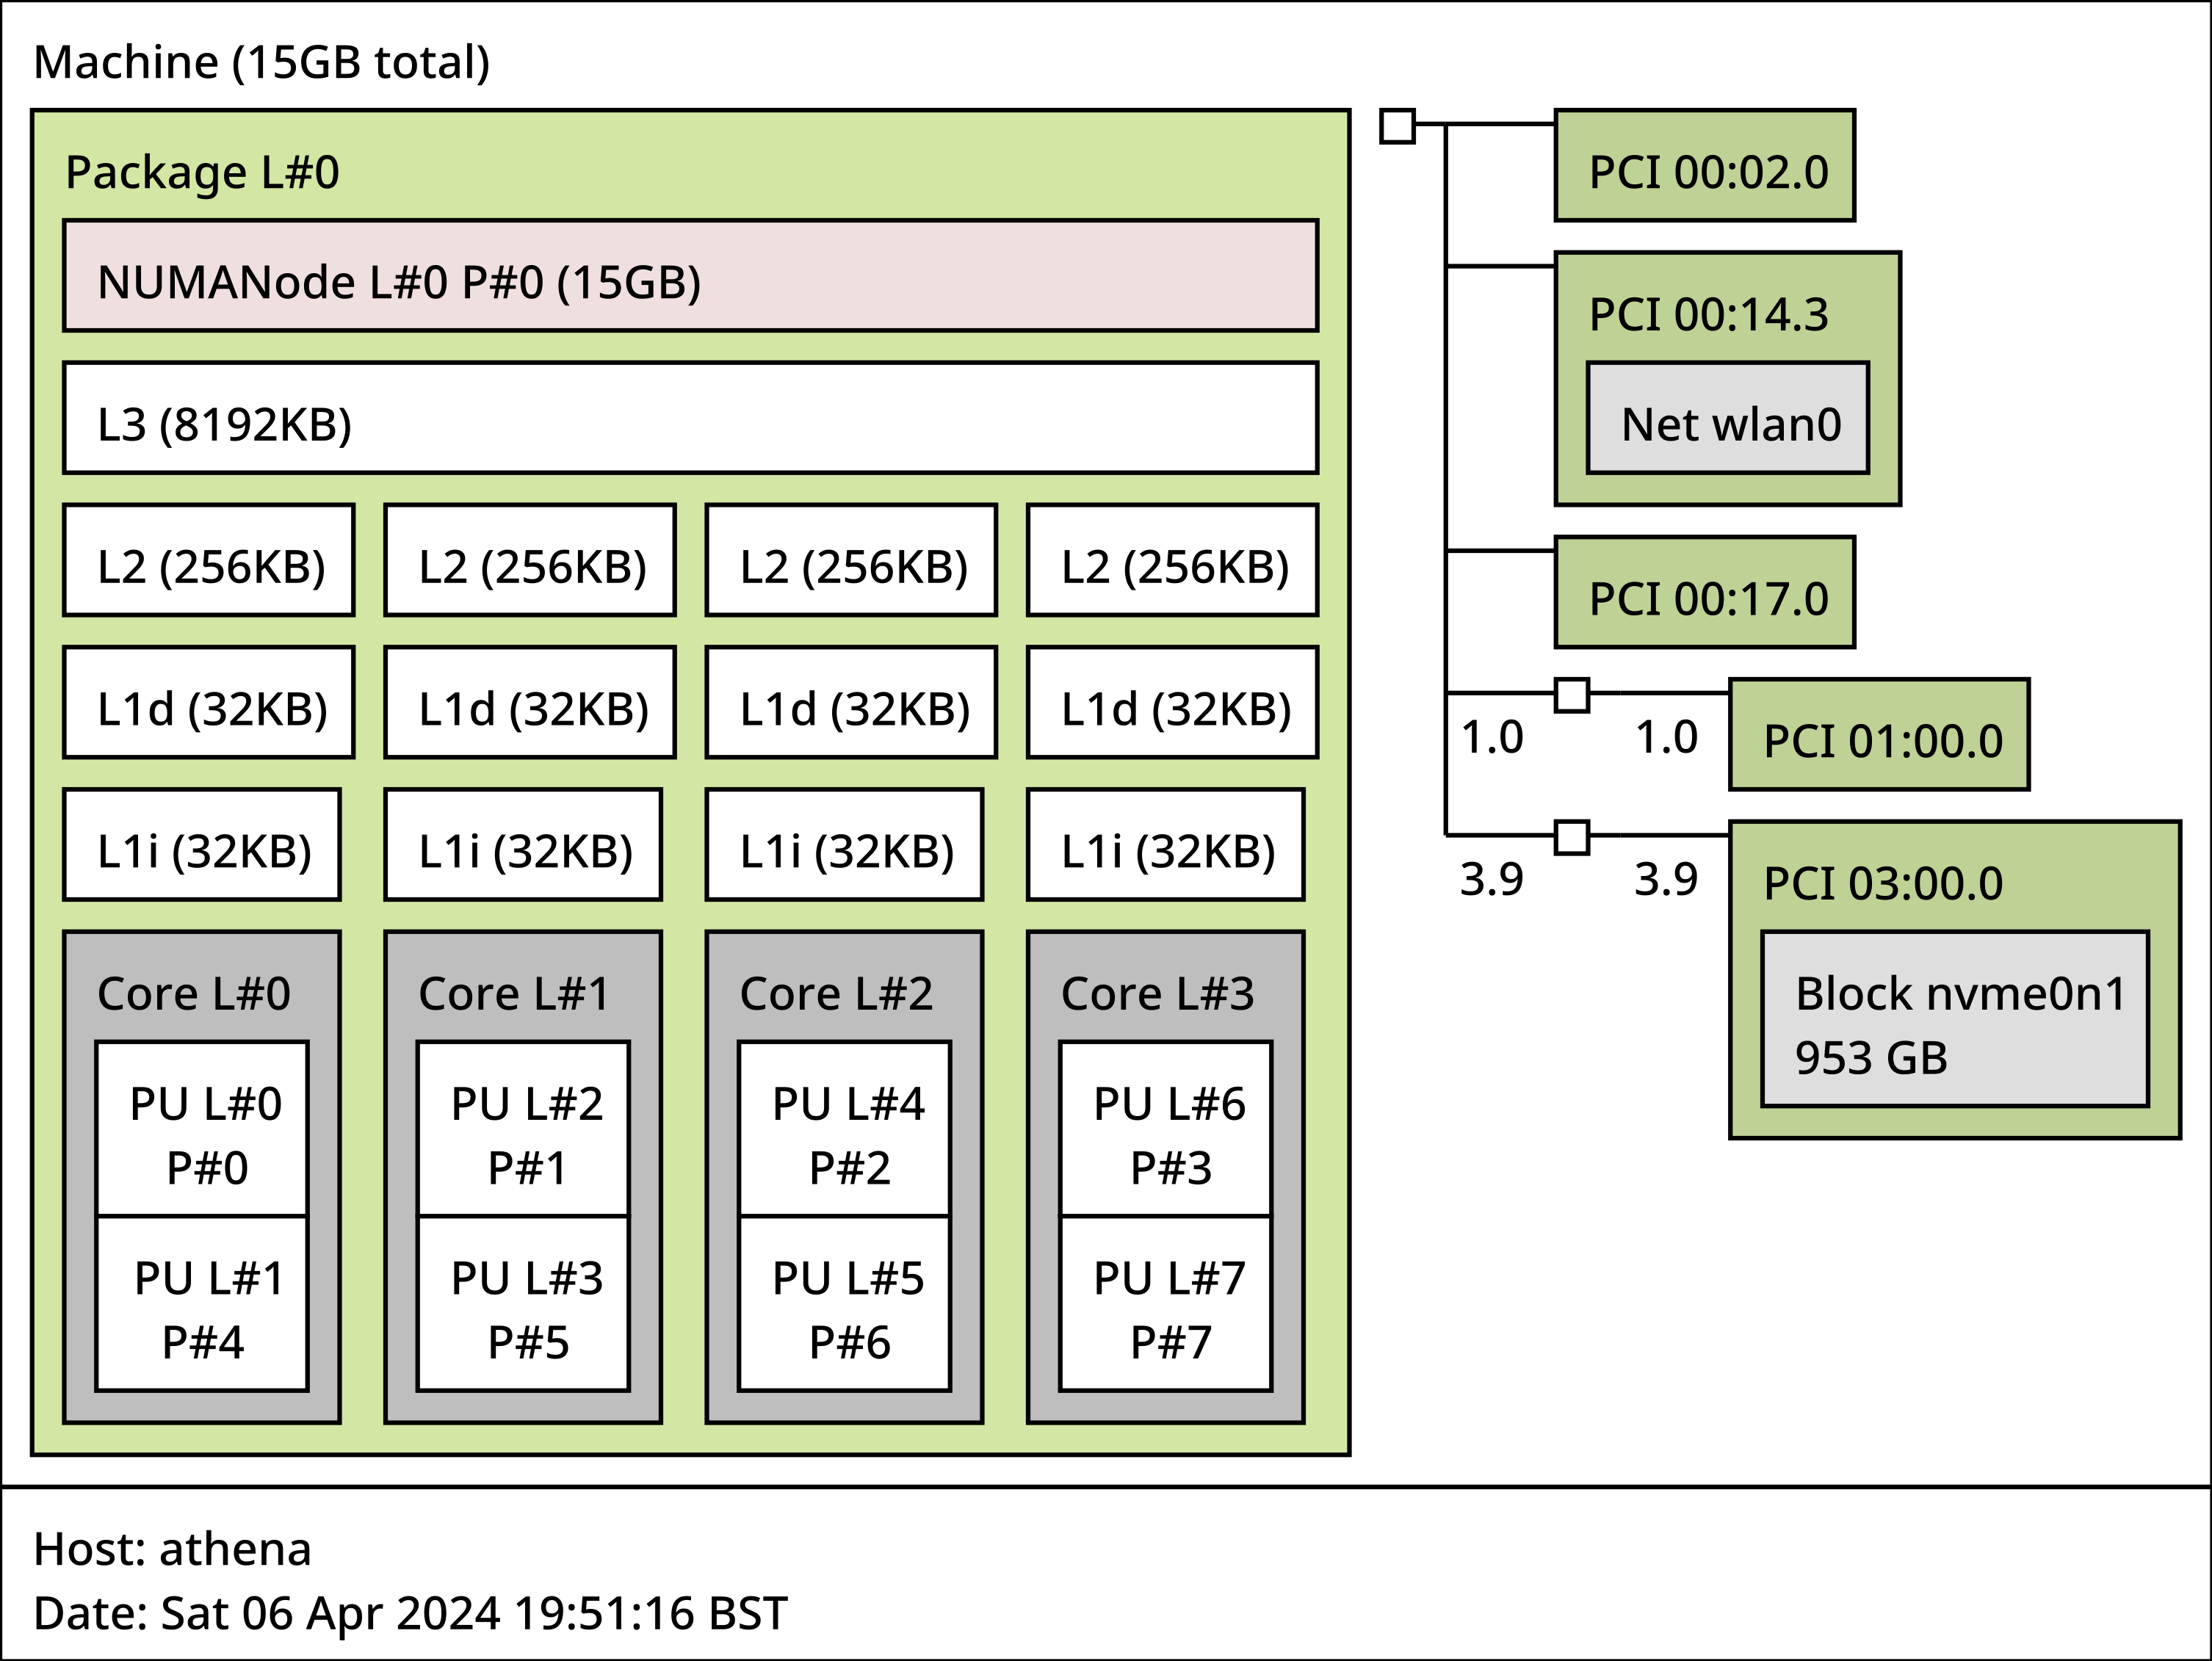
\includegraphics[width=0.75\textwidth]{images/8_appendix/athena-topology.png}
    \caption{A diagram of a hardware topology of Athena.}
    \label{fig:athena-topology}
\end{figure}

\begin{figure}[H]
    \centering
    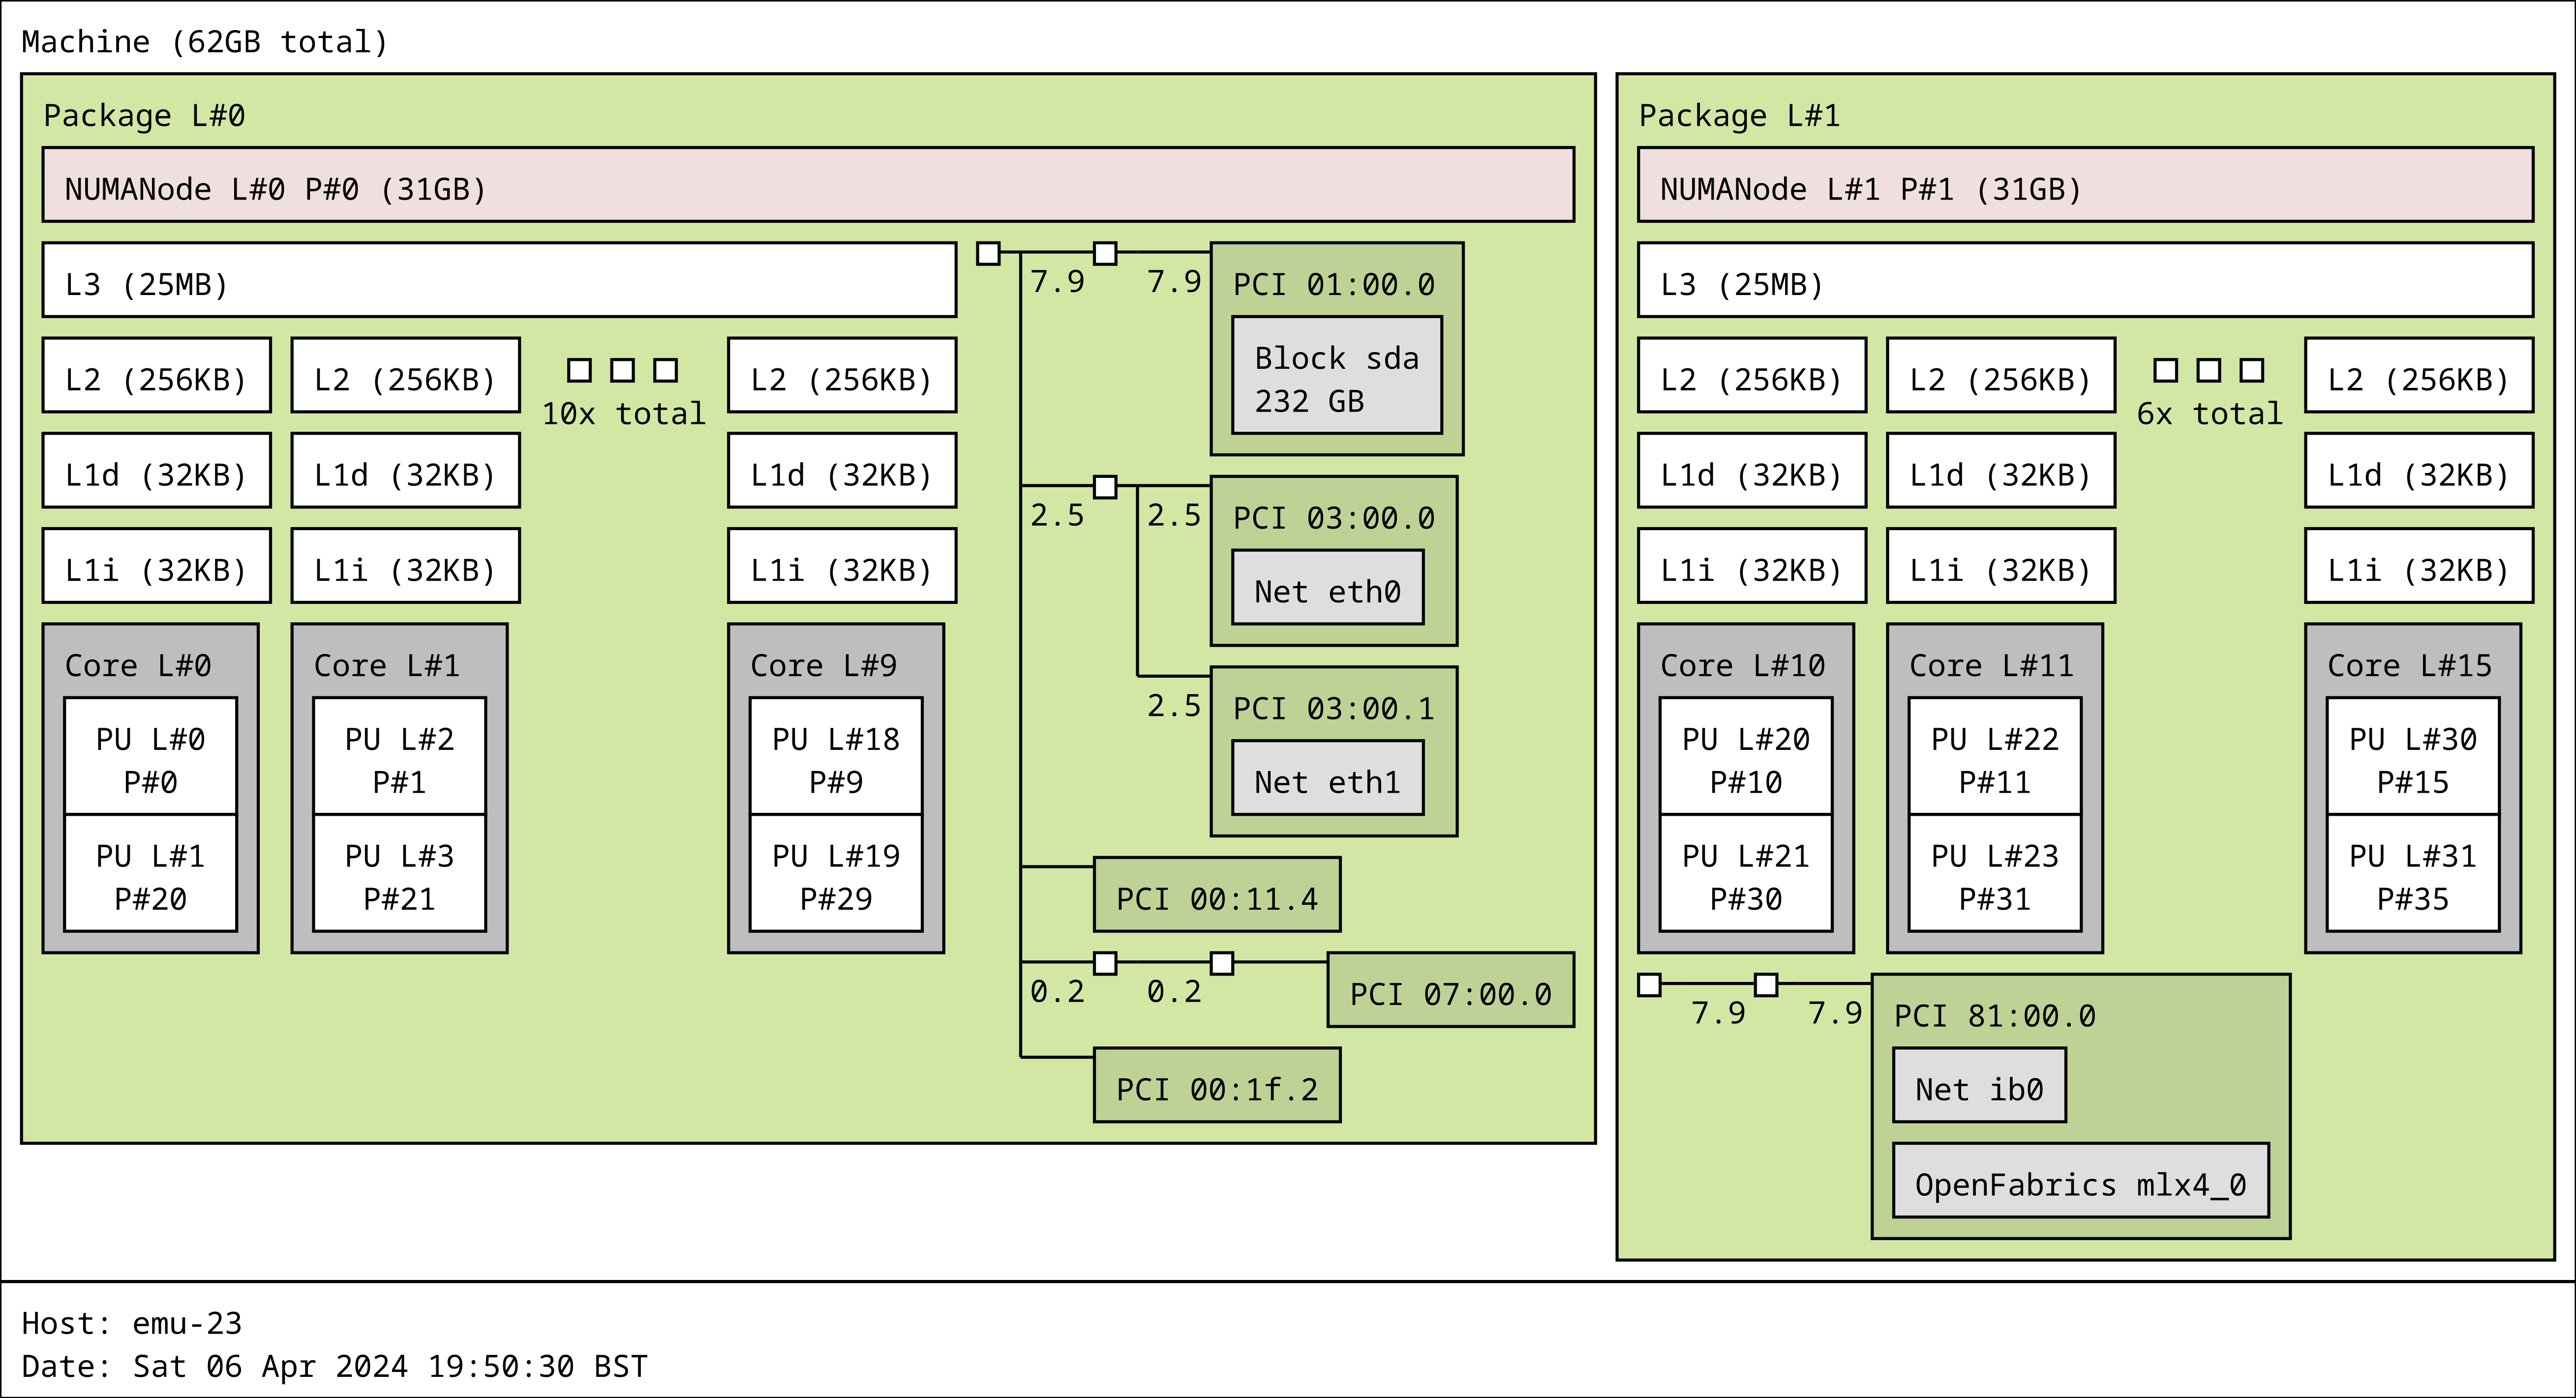
\includegraphics[width=0.85\textwidth]{images/8_appendix/kudu-topology.png}
    \caption{A diagram of a hardware topology of Kudu.}
    \label{fig:kudu-topology}
\end{figure}

\begin{figure}[H]
    \centering
    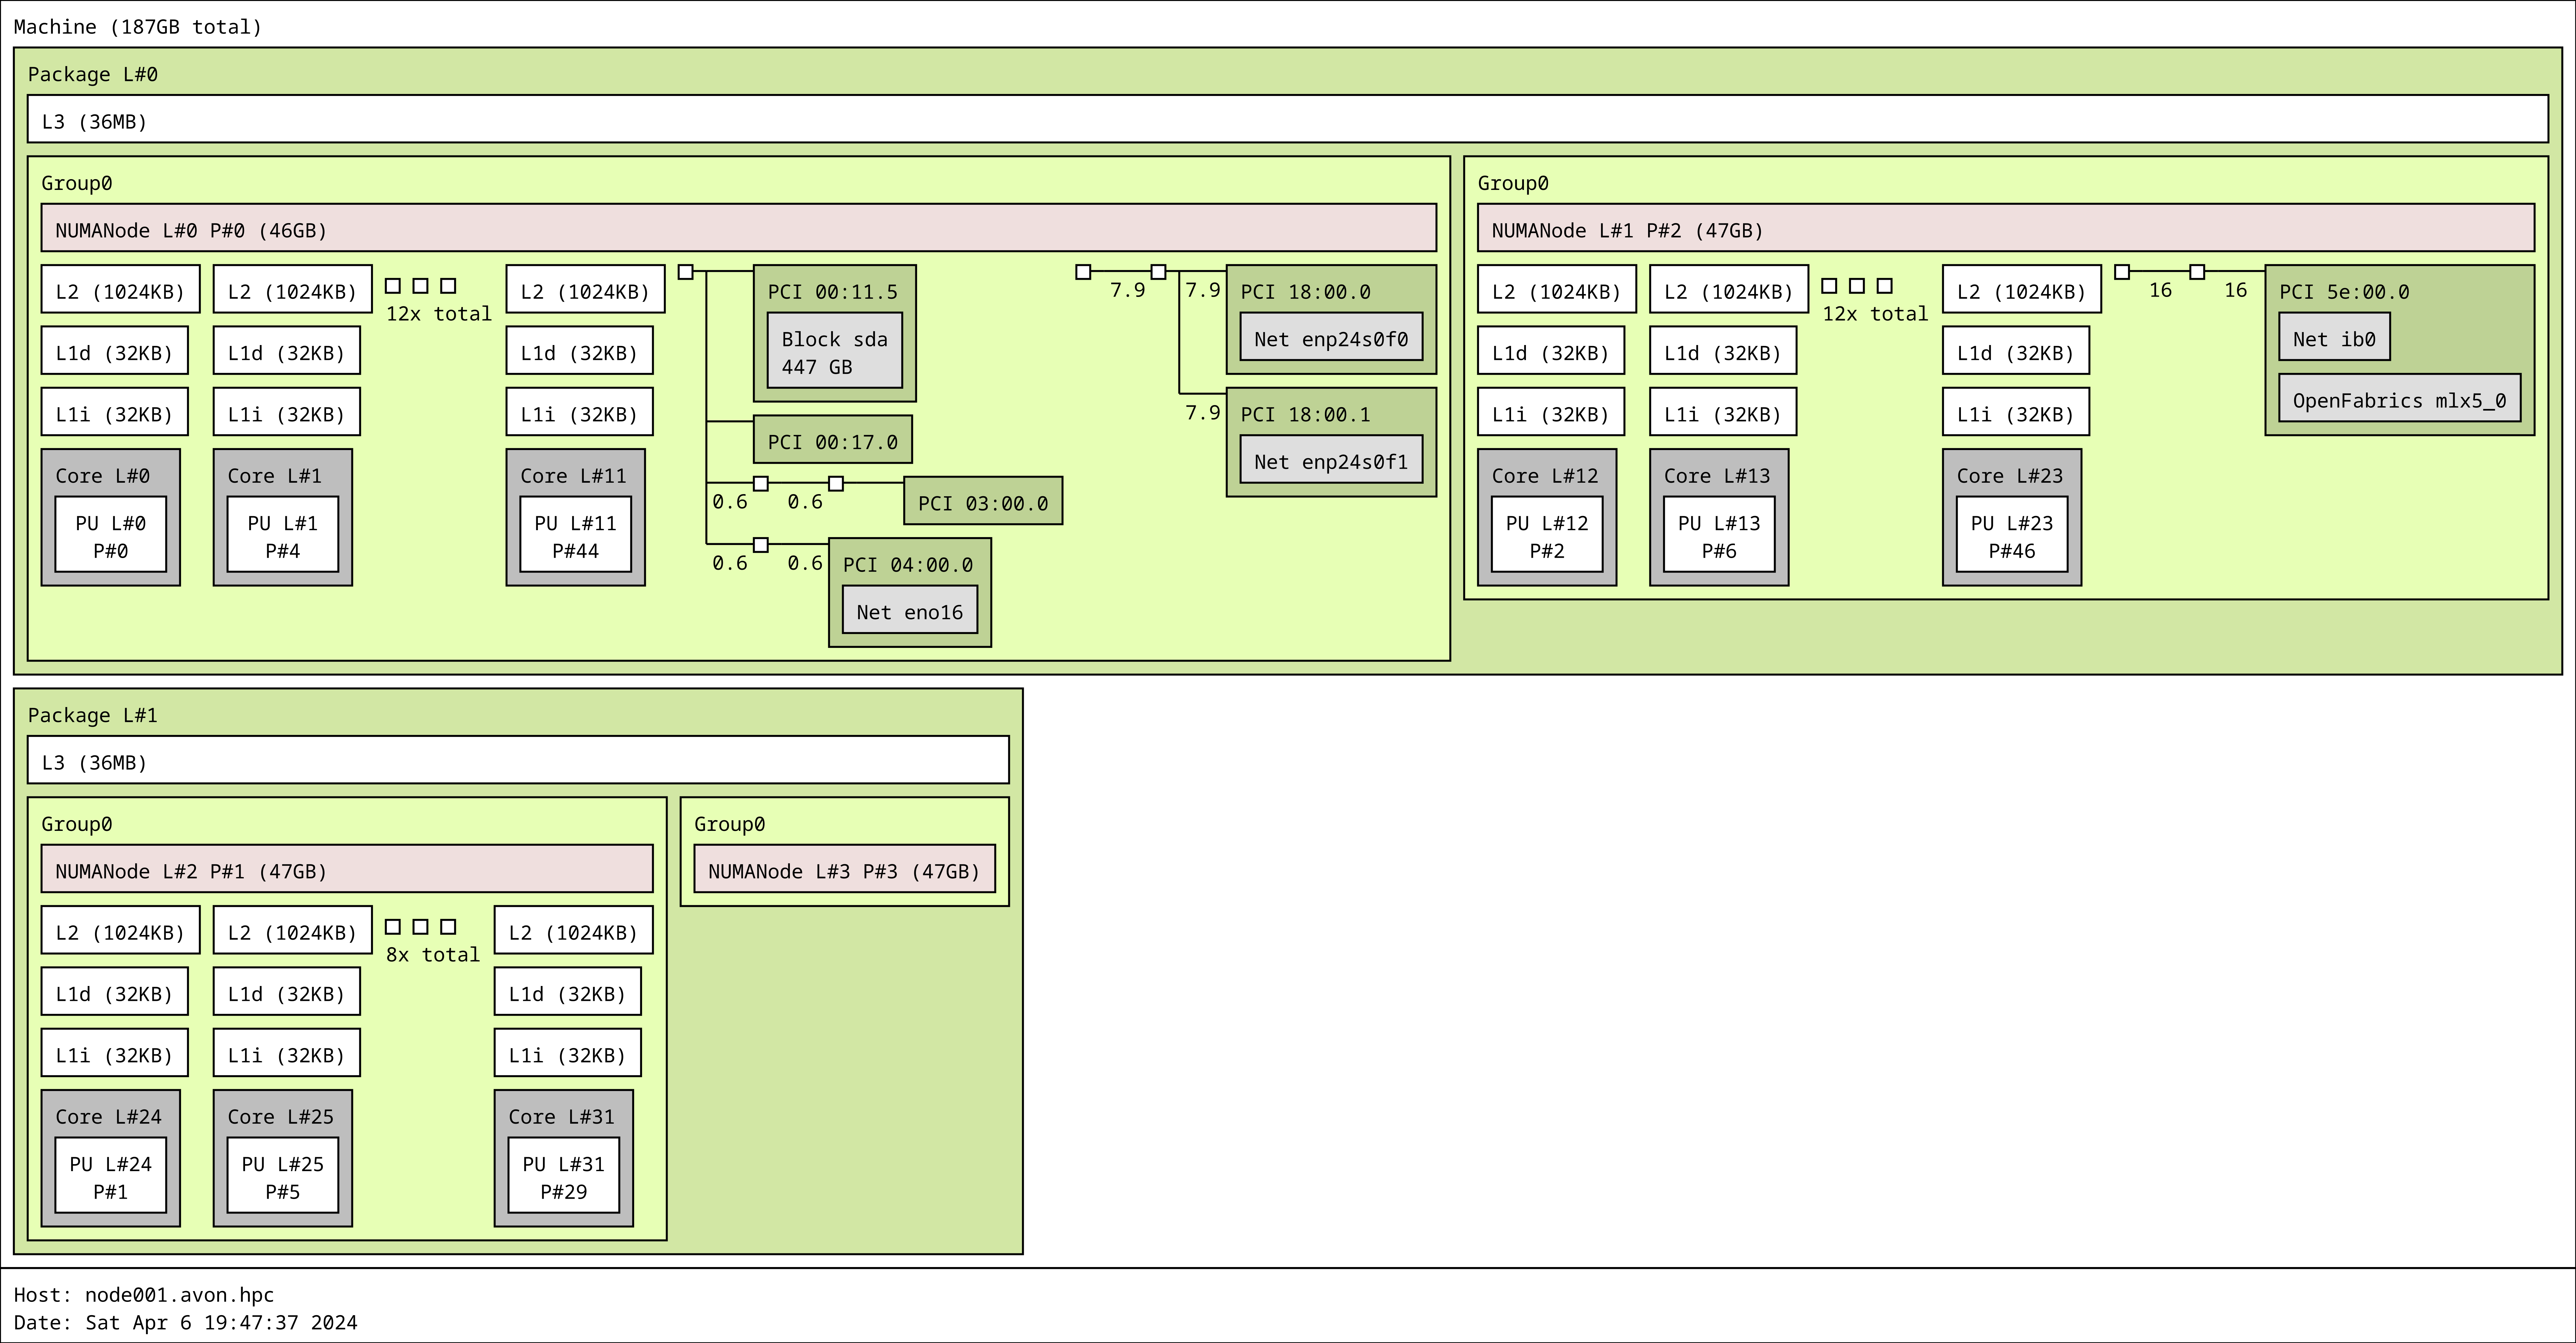
\includegraphics[width=0.95\textwidth]{images/8_appendix/avon-topology.png}
    \caption{A diagram of a hardware topology of Avon.}
    \label{fig:avon-topology}
\end{figure}

The results of running \texttt{lscpu} on the compute nodes for each of the systems are shown below in Listings \ref{listing:athena-lscpu}, \ref{listing:kudu-lscpu}, and \ref{listing:avon-lscpu}.

\begin{listing}[H]
    \begin{minted}[linenos,breaklines]{text}
Architecture:             x86_64
  CPU op-mode(s):         32-bit, 64-bit
  Address sizes:          39 bits physical, 48 bits virtual
  Byte Order:             Little Endian
CPU(s):                   8
  On-line CPU(s) list:    0-7
Vendor ID:                GenuineIntel
  Model name:             Intel(R) Core(TM) i7-8565U CPU @ 1.80GHz
    CPU family:           6
    Model:                142
    Thread(s) per core:   2
    Core(s) per socket:   4
    Socket(s):            1
    Stepping:             12
    CPU(s) scaling MHz:   21%
    CPU max MHz:          4600.0000
    CPU min MHz:          400.0000
    BogoMIPS:             4001.60
    Flags:                fpu vme de pse tsc msr pae mce cx8 apic sep mtrr pge mca cmov pat pse36 clflush dts acpi mmx fxsr sse sse2 ss ht tm pbe syscall nx pdpe1gb rdtscp lm constant_tsc art 
                          arch_perfmon pebs bts rep_good nopl xtopology nonstop_tsc cpuid aperfmperf pni pclmulqdq dtes64 monitor ds_cpl vmx est tm2 ssse3 sdbg fma cx16 xtpr pdcm pcid sse4_1 s
                          se4_2 x2apic movbe popcnt tsc_deadline_timer aes xsave avx f16c rdrand lahf_lm abm 3dnowprefetch cpuid_fault epb ssbd ibrs ibpb stibp ibrs_enhanced tpr_shadow flexpri
                          ority ept vpid ept_ad fsgsbase tsc_adjust sgx bmi1 avx2 smep bmi2 erms invpcid mpx rdseed adx smap clflushopt intel_pt xsaveopt xsavec xgetbv1 xsaves dtherm ida arat 
                          pln pts hwp hwp_notify hwp_act_window hwp_epp vnmi md_clear flush_l1d arch_capabilities
Virtualization features:  
  Virtualization:         VT-x
Caches (sum of all):      
  L1d:                    128 KiB (4 instances)
  L1i:                    128 KiB (4 instances)
  L2:                     1 MiB (4 instances)
  L3:                     8 MiB (1 instance)
NUMA:                     
  NUMA node(s):           1
  NUMA node0 CPU(s):      0-7
Vulnerabilities:          
  Gather data sampling:   Mitigation; Microcode
  Itlb multihit:          KVM: Mitigation: VMX disabled
  L1tf:                   Not affected
  Mds:                    Not affected
  Meltdown:               Not affected
  Mmio stale data:        Mitigation; Clear CPU buffers; SMT vulnerable
  Reg file data sampling: Not affected
  Retbleed:               Mitigation; Enhanced IBRS
  Spec rstack overflow:   Not affected
  Spec store bypass:      Mitigation; Speculative Store Bypass disabled via prctl
  Spectre v1:             Mitigation; usercopy/swapgs barriers and __user pointer sanitization
  Spectre v2:             Mitigation; Enhanced / Automatic IBRS, IBPB conditional, RSB filling, PBRSB-eIBRS SW sequence
  Srbds:                  Mitigation; Microcode
  Tsx async abort:        Not affected
    \end{minted}
    \caption{The output of the \texttt{lscpu} command on Athena.}
    \label{listing:athena-lscpu}
\end{listing}

\begin{listing}[H]
    \begin{minted}[linenos,breaklines]{text}
Architecture:        x86_64
CPU op-mode(s):      32-bit, 64-bit
Byte Order:          Little Endian
CPU(s):              40
On-line CPU(s) list: 0-39
Thread(s) per core:  2
Core(s) per socket:  10
Socket(s):           2
NUMA node(s):        2
Vendor ID:           GenuineIntel
CPU family:          6
Model:               63
Model name:          Intel(R) Xeon(R) CPU E5-2660 v3 @ 2.60GHz
Stepping:            2
CPU MHz:             3300.000
CPU max MHz:         3300.0000
CPU min MHz:         1200.0000
BogoMIPS:            5199.67
Virtualization:      VT-x
L1d cache:           32K
L1i cache:           32K
L2 cache:            256K
L3 cache:            25600K
NUMA node0 CPU(s):   0-9,20-29
NUMA node1 CPU(s):   10-19,30-39
Flags:               fpu vme de pse tsc msr pae mce cx8 apic sep mtrr pge mca cmov pat pse36 clflush dts acpi mmx fxsr sse sse2 ss ht tm pbe syscall nx pdpe1gb rdtscp lm constant_tsc arch_perfmon pebs bts rep_good nopl xtopology nonstop_tsc cpuid aperfmperf pni pclmulqdq dtes64 monitor ds_cpl vmx smx est tm2 ssse3 sdbg fma cx16 xtpr pdcm pcid dca sse4_1 sse4_2 x2apic movbe popcnt tsc_deadline_timer aes xsave avx f16c rdrand lahf_lm abm cpuid_fault epb invpcid_single pti intel_ppin ssbd ibrs ibpb stibp tpr_shadow vnmi flexpriority ept vpid ept_ad fsgsbase tsc_adjust bmi1 avx2 smep bmi2 erms invpcid cqm xsaveopt cqm_llc cqm_occup_llc dtherm ida arat pln pts md_clear flush_l1d
    \end{minted}
    \caption{The output of the \texttt{lscpu} command on the Kudu compute node.}
    \label{listing:kudu-lscpu}
\end{listing}

\begin{listing}[H]
    \begin{minted}[linenos,breaklines]{text}
Architecture:        x86_64
CPU op-mode(s):      32-bit, 64-bit
Byte Order:          Little Endian
CPU(s):              48
On-line CPU(s) list: 0-47
Thread(s) per core:  1
Core(s) per socket:  24
Socket(s):           2
NUMA node(s):        4
Vendor ID:           GenuineIntel
CPU family:          6
Model:               85
Model name:          Intel(R) Xeon(R) Platinum 8268 CPU @ 2.90GHz
Stepping:            7
CPU MHz:             3506.916
BogoMIPS:            5800.00
Virtualization:      VT-x
L1d cache:           32K
L1i cache:           32K
L2 cache:            1024K
L3 cache:            36608K
NUMA node0 CPU(s):   0,4,8,12,16,20,24,28,32,36,40,44
NUMA node1 CPU(s):   1,5,9,13,17,21,25,29,33,37,41,45
NUMA node2 CPU(s):   2,6,10,14,18,22,26,30,34,38,42,46
NUMA node3 CPU(s):   3,7,11,15,19,23,27,31,35,39,43,47
Flags:               fpu vme de pse tsc msr pae mce cx8 apic sep mtrr pge mca cmov pat pse36 clflush dts acpi mmx fxsr sse sse2 ss ht tm pbe syscall nx pdpe1gb rdtscp lm constant_tsc art arch_perfmon pebs bts rep_good nopl xtopology nonstop_tsc cpuid aperfmperf pni pclmulqdq dtes64 monitor ds_cpl vmx smx est tm2 ssse3 sdbg fma cx16 xtpr pdcm pcid dca sse4_1 sse4_2 x2apic movbe popcnt tsc_deadline_timer aes xsave avx f16c rdrand lahf_lm abm 3dnowprefetch cpuid_fault epb cat_l3 cdp_l3 invpcid_single intel_ppin ssbd mba ibrs ibpb stibp ibrs_enhanced fsgsbase tsc_adjust bmi1 hle avx2 smep bmi2 erms invpcid cqm mpx rdt_a avx512f avx512dq rdseed adx smap clflushopt clwb intel_pt avx512cd avx512bw avx512vl xsaveopt xsavec xgetbv1 xsaves cqm_llc cqm_occup_llc cqm_mbm_total cqm_mbm_local dtherm ida arat pln pts pku ospke avx512_vnni md_clear flush_l1d arch_capabilities
    \end{minted}
    \caption{The output of the \texttt{lscpu} command on Athena.}
    \label{listing:avon-lscpu}
\end{listing}

%TC:endignore

\end{document}
